\chapter{Sayısal Tasarım Temelleri}
\label{ch:sayisal-tasarim}
\bolumfoto[Galata Kulesi, taş taş üstüne koyularak yükselmiştir. Sayısal devreler de kapı kapı üstüne koyularak inşa edilir: VE, VEYA ve DEĞİL kapılarından toplayıcılara, yazmaçlara ve sonunda bütün bir işlemciye.]{gorseller/ekB-galatakulesi.jpg}{Galata Kulesi -- İstanbul}

\begin{tcolorbox}[
    colback=blokyesil!15,
    colframe=sinyalyesil!60!black,
    title={\textbf{Öğrenme Hedefleri}},
    fonttitle=\bfseries,
    rounded corners,
    boxrule=0.8pt
]
Bu eki tamamladığınızda aşağıdakileri yapabileceksiniz:
\begin{itemize}[nosep, leftmargin=*]
    \item Temel mantık kapılarının (VE, VEYA, DEĞİL) ve türetilmiş kapıların (VE-DEĞİL, VEYA-DEĞİL, Dışlayan VEYA, Dışlayan VEYA DEĞİL) doğruluk tablolarını yazmak.
    \item Boole cebri kurallarını ve De Morgan kuramlarını kullanarak mantık ifadelerini sadeleştirmek.
    \item Karno haritası yöntemiyle 2, 3, 4, 5 ve 6 değişkenli fonksiyonları en yalın biçimlerine indirgemek.
    \item Önemsenmeyen durumların Karno haritasında nasıl kullanıldığını açıklamak.
    \item Quine--McCluskey algoritmasıyla herhangi bir sayıda değişkenli fonksiyonu sadeleştirmek.
    \item Toplayıcı, kod çözücü ve çoklayıcı devrelerinin yapısını ve işleyişini tanımlamak.
    \item RS, D, T ve JK flip-floplarının çalışma ilkelerini karşılaştırmak.
    \item Yazmaç ve sayaç devrelerinin flip-floplardan nasıl oluşturulduğunu göstermek.
    \item Mealy ve Moore durum makineleri arasındaki farkları açıklamak ve basit bir durum makinesi tasarlamak.
\end{itemize}
\end{tcolorbox}

\section{Giriş}

Bir bilgisayarı anlamak, onu oluşturan soyutlama katmanlarını tanımakla başlar. Bölüm~\ref{chap:islemci-tasarimi} ve Bölüm~\ref{chap:boruhatti}'de işlemci, AMB, yazmaç öbeği ve bellek gibi birimler birer kutu olarak çizilmiştir. Bu kutular Yazmaç Aktarım Seviyesi'nde (YAS) tasarlanır; ancak her kutunun içinde mantık kapılarından örülmüş bir devre yatar. Tıpkı bölüm fotoğrafındaki Galata Kulesi'nin taş taş üstüne yükselmesi gibi, bir işlemci de VE, VEYA ve DEĞİL kapılarının üst üste eklenmesiyle inşa edilir.

Sayısal tasarım kavramları kitabın birçok bölümünde karşımıza çıkar: Bölüm~\ref{chap:aritmetik}'te toplayıcı ve çarpıcı devreleri mantık kapılarından kurulur; Bölüm~\ref{chap:islemci-tasarimi}'da veriyolu çoklayıcıları ve denetim birimi Boole ifadeleriyle tasarlanır; Bölüm~\ref{chap:boruhatti}'de boru hattı yazmaçları flip-floplardan oluşur; Bölüm~\ref{chap:bellek}'de önbellek denetleyicisi bir durum makinesidir. Bu nedenle sayısal tasarım temelleri, kitabın tamamını destekleyen ortak bir altyapıdır.

Bu ek, sayısal tasarım dersini daha önce almış okuyucular için bir anımsatıcı; henüz almamış olanlar için ise bağımsız bir başlangıç kaynağı olarak tasarlanmıştır. Amaç, kitabın ana bölümlerini takip edebilmek için gereken asgari sayısal tasarım bilgisini tek bir yerde toplamaktır.

Sayısal tasarım, \textbf{birleşik}\index{birleşik devre} (İngilizcesi: \textit{combinational}) ve \textbf{ardışıl}\index{ardışıl devre} (İngilizcesi: \textit{sequential}) olmak üzere iki temel devre sınıfı üzerine kuruludur. Birleşik devrelerde çıkış yalnızca o andaki girişlere bağlıdır; mantık kapıları, toplayıcılar ve çoklayıcılar bu gruptadır. Ardışıl devrelerde ise çıkış hem girişlere hem de devrenin o anki \emph{durumuna} bağlıdır; flip-floplar, yazmaçlar ve sayaçlar bu gruba girer. Bir işlemci, bu iki sınıfın iç içe geçmesiyle oluşur: veriyolundaki AMB birleşik bir devredir, onu besleyen yazmaçlar ise ardışıl devrelerdir. Bu ekin ilk yarısı birleşik yapı taşlarını, ikinci yarısı ardışıl yapı taşlarını ele almaktadır.

\begin{terimnotu}
\textbf{birleşik devre} (\emph{combinational circuit})\,: \emph{Birleşmek} fiilinden. Çıkış yalnızca girişlerin o anki \emph{birleşimine} bağlıdır; bellek tutmaz. Türkçe kaynaklarda sıklıkla ``kombinasyonel devre'' olarak geçer; ancak ``kombinasyonel'' Türkçe bir sözcük değildir, İngilizce \emph{combinational} sözcüğünün doğrudan aktarımıdır. Bu kitapta \emph{birleşik} terimi kullanılmaktadır.\\[4pt]
\textbf{ardışıl devre} (\emph{sequential circuit})\,: \emph{Ardışık} (consecutive) kökünden. Çıkış hem girişlere hem de devrenin \emph{durumuna} bağlıdır; flip-floplarla bellek tutar. ``Sıralı devre'' de kullanılır; bu kitapta \emph{ardışıl} tercih edilmiştir.
\end{terimnotu}

\begin{bilginot}[Sayısal Tasarım ve Teknoloji]
Bu ekte anlatılan mantık kapıları, Boole cebri ve devre tasarım ilkeleri bugün CMOS\index{CMOS} (\emph{Complementary Metal-Oxide-Semiconductor}) transistör teknolojisi üzerine kuruludur. CMOS, 1960'lardan bu yana yarı iletken endüstrisinin temel yapı taşıdır ve günümüzdeki tüm işlemciler, bellekler ve sayısal tümleşik devreler bu teknolojiyle üretilir.

Ancak CMOS tek olasılık değildir. Tarihte röleler, vakum tüpleri ve ayrık transistörler de mantık kapıları gerçekleştirmek için kullanılmıştır. Gelecekte ise kuantum hesaplama\index{kuantum hesaplama}, spintronic veya fotonik gibi yeni teknolojiler farklı temel yapı taşları sunabilir; örneğin kuantum bilgisayarlarda klasik VE/VEYA kapıları yerine kuantum kapıları (Hadamard, CNOT, Toffoli) kullanılır ve Boole cebri yerine doğrusal cebir devreye girer. Bu ekteki ilkeler CMOS teknolojisine özgü değildir; Boole cebri ve durum makineleri gibi soyutlamalar, altlarındaki fiziksel teknoloji değişse bile geçerli kalır. Değişen, bu soyutlamaların donanımda nasıl gerçekleştirildiğidir.
\end{bilginot}

Ekte sırasıyla şu konular ele alınmaktadır:

\begin{itemize}[nosep]
    \item Mantık kapıları ve doğruluk tabloları
    \item Boole cebri, De Morgan kuramları ve Karno haritalarıyla fonksiyon sadeleştirme
    \item Quine--McCluskey algoritması
    \item Birleşik yapı taşları: toplayıcılar, kod çözücüler ve çoklayıcılar
    \item Birleşik tasarım örneği
    \item Flip-floplar, yazmaçlar ve sayaçlar
    \item Mealy ve Moore durum makineleri
    \item Ardışıl tasarım örnekleri
\end{itemize}

\noindent İkilik tabandaki sayı gösterimleri, taban dönüşümleri ve işaretli sayı aritmetiği Ek~\ref{ch:sayi-sistemleri}'da ayrıntılı olarak ele alınmıştır.


\section{Mantık Kapıları ve Doğruluk Tabloları}

\subsection{İkilik Sistem ve Mantık}

Bilgisayarlar ikilik sistemde çalışır: her basamak yalnızca 0 veya 1 değerini alır. Fiziksel düzeyde bu iki değer genellikle düşük ve yüksek gerilim seviyeleriyle temsil edilir. Aynı zamanda mantıktaki \emph{yanlış} ve \emph{doğru} kavramlarına karşılık gelirler. Sayısal tasarım, bu iki değer üzerinde işlem yapan devrelerin (mantık kapılarının) birleştirilerek karmaşık sistemler oluşturulmasıdır. İkilik sayı gösterimleri, taban dönüşümleri, işaretli sayılar ve ikiye tümleyen yöntemi Ek~\ref{ch:sayi-sistemleri}'da ayrıntılı olarak ele alınmaktadır.


\subsection{Temel Kapılar ve Devre Sembolleri}

Mantık kapıları, temel mantık fonksiyonlarını gerçekleştiren, transistörlerden oluşmuş devrelerdir. Üç temel mantık kapısı şunlardır:

\begin{itemize}[nosep]
    \item \textbf{VE (AND):} Çıkış, ancak \emph{tüm} girişler 1 olduğunda 1 olur. Günlük hayattan bir benzetme: bir kapı, ancak hem anahtar \emph{ve} hem şifre doğruysa açılır.
    \item \textbf{VEYA (OR):} Çıkış, girişlerden \emph{en az biri} 1 olduğunda 1 olur. Benzetme: bir alarm, kapı \emph{veya} pencere açılırsa çalar.
    \item \textbf{DEĞİL (NOT):} Tek girişli bir kapıdır; girişin tersini üretir. 0 girerse 1, 1 girerse 0 çıkar.
\end{itemize}

Bu üç kapıdan türetilen VE-DEĞİL (NAND), VEYA-DEĞİL (NOR), Dışlayan VEYA (XOR) ve Dışlayan VEYA DEĞİL (XNOR) kapıları da yaygın olarak kullanılır.

Bir mantık kapısının davranışı \textbf{doğruluk tablosu}\index{doğruluk tablosu} ile tanımlanır: tablonun her satırı olası bir giriş kombinasyonunu, karşısındaki sütun ise o kombinasyon için üretilen çıkış değerini gösterir. $n$ girişli bir kapının doğruluk tablosu $2^n$ satırdan oluşur: 2 girişli bir kapı için 4, 3 girişli bir fonksiyon için 8, 4 girişli bir fonksiyon için 16 satır gerekir. Aşağıdaki tablolarda ve şekilde yedi temel kapının doğruluk tabloları ve devre sembolleri verilmiştir.

\begin{terimnotu}
\textbf{Dışlayan VEYA} (\emph{Exclusive OR}, XOR)\index{Dışlayan VEYA}\index{XOR|see{Dışlayan VEYA}}\,: Türkçede sıklıkla ``Özel VEYA'' olarak anılır; ancak \emph{exclusive} sözcüğünün doğru karşılığı ``dışlayan''dır. İşlemin mantığı bu adı açıklar: iki giriş \emph{aynı} ise sonuç 0 olur, aynı değerler \emph{dışlanır}. Yalnızca girişler farklı olduğunda sonuç 1 olur. Boole cebirinde $A \oplus B$ ile gösterilir.\\[4pt]
\textbf{Dışlayan VEYA DEĞİL} (\emph{Exclusive NOR}, XNOR)\index{Dışlayan VEYA DEĞİL}\index{XNOR|see{Dışlayan VEYA DEĞİL}}\,: Dışlayan VEYA'nın tersidir. Girişler \emph{aynı} olduğunda 1, farklı olduğunda 0 üretir; bir eşitlik denetleyicisidir. $\overline{A \oplus B}$ ile gösterilir.
\end{terimnotu}

\begin{table}[H]
\centering
\begin{minipage}{0.3\textwidth}
\centering
\textbf{VE Kapısı}
\vspace{0.3em}

\begin{tabular}{cc|c}
\toprule
\textbf{A} & \textbf{B} & \textbf{C} \\
\midrule
0 & 0 & 0 \\
0 & 1 & 0 \\
1 & 0 & 0 \\
1 & 1 & 1 \\
\bottomrule
\end{tabular}
\end{minipage}
\hfill
\begin{minipage}{0.3\textwidth}
\centering
\textbf{VEYA Kapısı}
\vspace{0.3em}

\begin{tabular}{cc|c}
\toprule
\textbf{A} & \textbf{B} & \textbf{C} \\
\midrule
0 & 0 & 0 \\
0 & 1 & 1 \\
1 & 0 & 1 \\
1 & 1 & 1 \\
\bottomrule
\end{tabular}
\end{minipage}
\hfill
\begin{minipage}{0.3\textwidth}
\centering
\textbf{DEĞİL Kapısı}
\vspace{0.3em}

\begin{tabular}{c|c}
\toprule
\textbf{A} & \textbf{B} \\
\midrule
0 & 1 \\
1 & 0 \\
\bottomrule
\end{tabular}
\end{minipage}
\end{table}

\begin{figure}[H]
\centering
\begin{tikzpicture}[kapiboy, scale=0.85, transform shape]
  % --- Üst satır: VE, VEYA, DEĞİL ---
  % AND kapısı
  \node[and gate US, draw, thick, fill=blokgri] (and) at (0,0) {};
  \draw (and.input 1) -- ++(-0.6,0) node[left] {\footnotesize $A$};
  \draw (and.input 2) -- ++(-0.6,0) node[left] {\footnotesize $B$};
  \draw (and.output) -- ++(0.6,0) node[right] {\footnotesize $A \cdot B$};
  \node[below=4pt] at (and.south) {\footnotesize VE (AND)};

  % OR kapısı
  \node[or gate US, draw, thick, fill=blokgri] (or) at (4.5,0) {};
  \draw (or.input 1) -- ++(-0.6,0) node[left] {\footnotesize $A$};
  \draw (or.input 2) -- ++(-0.6,0) node[left] {\footnotesize $B$};
  \draw (or.output) -- ++(0.6,0) node[right] {\footnotesize $A + B$};
  \node[below=4pt] at (or.south) {\footnotesize VEYA (OR)};

  % DEĞİL kapısı
  \node[not gate US, draw, thick, fill=blokgri] (not) at (9,0) {};
  \draw (not.input) -- ++(-0.6,0) node[left] {\footnotesize $A$};
  \draw (not.output) -- ++(0.6,0) node[right] {\footnotesize $\overline{A}$};
  \node[below=4pt] at (not.south) {\footnotesize DEĞİL (NOT)};

  % --- Orta satır: NAND, NOR ---
  % NAND kapısı
  \node[nand gate US, draw, thick, fill=blokgri] (nand) at (0,-3) {};
  \draw (nand.input 1) -- ++(-0.6,0) node[left] {\footnotesize $A$};
  \draw (nand.input 2) -- ++(-0.6,0) node[left] {\footnotesize $B$};
  \draw (nand.output) -- ++(0.6,0) node[right] {\footnotesize $\overline{A \cdot B}$};
  \node[below=4pt] at (nand.south) {\footnotesize VE DEĞİL (NAND)};

  % NOR kapısı
  \node[nor gate US, draw, thick, fill=blokgri] (nor) at (4.5,-3) {};
  \draw (nor.input 1) -- ++(-0.6,0) node[left] {\footnotesize $A$};
  \draw (nor.input 2) -- ++(-0.6,0) node[left] {\footnotesize $B$};
  \draw (nor.output) -- ++(0.6,0) node[right] {\footnotesize $\overline{A + B}$};
  \node[below=4pt] at (nor.south) {\footnotesize VEYA DEĞİL (NOR)};

  % --- Alt satır: XOR, XNOR ---
  % XOR kapısı
  \node[xor gate US, draw, thick, fill=blokgri] (xor) at (2.25,-6) {};
  \draw (xor.input 1) -- ++(-0.6,0) node[left] {\footnotesize $A$};
  \draw (xor.input 2) -- ++(-0.6,0) node[left] {\footnotesize $B$};
  \draw (xor.output) -- ++(0.6,0) node[right] {\footnotesize $A \oplus B$};
  \node[below=4pt] at (xor.south) {\footnotesize Dışlayan VEYA (XOR)};

  % XNOR kapısı
  \node[xnor gate US, draw, thick, fill=blokgri] (xnor) at (6.75,-6) {};
  \draw (xnor.input 1) -- ++(-0.6,0) node[left] {\footnotesize $A$};
  \draw (xnor.input 2) -- ++(-0.6,0) node[left] {\footnotesize $B$};
  \draw (xnor.output) -- ++(0.6,0) node[right] {\footnotesize $\overline{A \oplus B}$};
  \node[below=4pt] at (xnor.south) {\footnotesize Dışlayan VEYA DEĞİL (XNOR)};
\end{tikzpicture}
\caption{Temel ve türetilmiş mantık kapılarının devre sembolleri}
\label{fig:B.1}
\end{figure}

Giriş sayısı arttıkça doğruluk tablosu hızla büyür; bu nedenle ilerleyen bölümlerde tanıtılacak olan Boole cebri ve Karno haritası gibi yöntemler, fonksiyonların tablo çizmeden sadeleştirilmesini sağlar. Bu yedi kapı arasında özellikle VE-DEĞİL ve VEYA-DEĞİL kapıları ayrı bir öneme sahiptir: bu iki kapı \emph{evrensel} kapılardır; yalnızca bu kapılar kullanılarak diğer tüm kapılar gerçekleştirilebilir.

\subsection{Evrensel Kapılar: VE-DEĞİL ve VEYA-DEĞİL}

VE-DEĞİL (NAND) ve VEYA-DEĞİL (NOR) kapıları \textbf{evrensel kapı} olarak adlandırılır; çünkü bu kapılardan herhangi biri tek başına kullanılarak tüm temel mantık kapıları (VE, VEYA, DEĞİL) gerçekleştirilebilir ve dolayısıyla herhangi bir Boole fonksiyonu ifade edilebilir.

\begin{itemize}[nosep]
    \item \textbf{DEĞİL:} Bir VE-DEĞİL kapısının iki girişi birbirine bağlanırsa DEĞİL kapısı elde edilir: $\overline{x \cdot x} = \overline{x}$.
    \item \textbf{VE:} İki VE-DEĞİL kapısı art arda bağlanarak VE kapısı oluşturulabilir: önce $\overline{x \cdot y}$, ardından bu çıkışın DEĞİL'i alınarak $x \cdot y$ elde edilir.
    \item \textbf{VEYA:} $x + y = \overline{\overline{x} \cdot \overline{y}}$ eşitliğine göre (ilerleyen bölümlerde De Morgan kuramı olarak tanıtılacaktır) bu ifade üç VE-DEĞİL kapısıyla gerçekleştirilebilir.
\end{itemize}

Aynı mantık, VEYA-DEĞİL kapısı için de geçerlidir. Uygulamada VE-DEĞİL ve VEYA-DEĞİL kapıları, transistor düzeyinde VE ve VEYA kapılarından daha verimli üretilebildiği için entegre devre tasarımında yaygın olarak tercih edilir.


\section{Boole Cebri}

Doğruluk tabloları her durumu teker teker listeleyerek bir fonksiyonu tanımlar; ancak giriş sayısı arttıkça bu yöntem kullanışsızlaşır. Boole cebri, mantık fonksiyonlarını cebirsel ifadelerle göstermeye ve bu ifadeleri kurallara dayalı olarak sadeleştirmeye olanak tanır. 1854 yılında George Boole tarafından geliştirilen bu cebir, VE işlemini ``$\cdot$'' (çarpma benzeri), VEYA işlemini ``$+$'' (toplama benzeri) ve DEĞİL işlemini üst çizgi ($\overline{x}$) ile gösterir.

\begin{bilginot}[George Boole ve Mantığın Cebirleşmesi]
\index{Boole, George}
George Boole (1815--1864), İngiliz matematikçi ve mantıkçıdır. 1854'te yayımladığı \emph{An Investigation of the Laws of Thought}~\cite{boole1854} adlı yapıtında, mantıksal akıl yürütmenin cebirsel denklemlerle ifade edilebileceğini göstermiştir. Boole bu çalışmayı yaparken ne transistör ne de elektrikli devre diye bir şey vardı; ilk transistör ancak 1947'de icat edilecekti. Boole'un amacı, insan düşüncesinin kurallarını matematiksel olarak modellemekti.

Boole cebrinin donanım tasarımına uygulanabileceğini 1937'de Claude Shannon\index{Shannon, Claude} keşfetmiştir. Shannon, yüksek lisans tezinde~\cite{shannon1937} elektrik anahtarlarının (rölelerin) Boole cebrinin fiziksel bir gerçeklemesi olduğunu göstermiş ve böylece sayısal devre tasarımının kuramsal temelini atmıştır. Bugün aynı cebir CMOS transistörleriyle gerçeklenmektedir; ancak tarihte röleler, vakum tüpleri ve mekanik düzenekler de mantık kapılarını gerçekleştirmek için kullanılmıştır. Boole cebrinin gücü, altındaki fiziksel teknolojiden bağımsız olmasıdır.
\end{bilginot}

\begin{bilginot}[Boole Cebrinde Gösterim ve Öncelik]
Boole cebrinde ``$\cdot$'' işareti sıklıkla yazılmaz: $x \cdot y$ yerine kısaca $xy$ yazılır. Ayrıca VE işlemi, VEYA işleminden önce gelir (tıpkı aritmetikteki çarpmanın toplamadan önce gelmesi gibi). Örneğin $x + yz$ ifadesi $x + (y \cdot z)$ anlamına gelir.
\end{bilginot}

Boole cebrinin temel özellikleri (Huntington önermeleri) Tablo~\ref{tab:boole-ozellikleri}'nde verilmiştir.

\begin{table}[H]
\centering
\caption{Boole cebrinin temel özellikleri}
\label{tab:boole-ozellikleri}
\begin{tabular}{l l l}
\toprule
\textbf{Özellik} & \textbf{VEYA ($+$) biçimi} & \textbf{VE ($\cdot$) biçimi} \\
\midrule
Kapalılık      & $1 + 1 = 1$                          & $0 \cdot 0 = 0$ \\
Birim eleman   & $x + 0 = x$                          & $x \cdot 1 = x$ \\
Değişme        & $x + y = y + x$                      & $x \cdot y = y \cdot x$ \\
Dağılma        & $x + (y \cdot z) = (x+y) \cdot (x+z)$ & $x \cdot (y+z) = (x \cdot y) + (x \cdot z)$ \\
Ters           & $x + \overline{x} = 1$               & $x \cdot \overline{x} = 0$ \\
Etkisizlik     & $x + x = x$                          & $x \cdot x = x$ \\
Yutma          & $x + 1 = 1$                          & $x \cdot 0 = 0$ \\
Çift tümleyen  & $\overline{\overline{x}} = x$ & $\overline{\overline{x}} = x$ \\
\bottomrule
\end{tabular}
\end{table}

Tablodaki ikiliğe dikkat edilmelidir: her özelliğin bir VEYA biçimi, bir de VE biçimi vardır. Bu ikiliğe Boole cebrinde \emph{eşiklik} (\emph{duality}) denir: herhangi bir doğru ifadede ``$+$'' ile ``$\cdot$''yi ve ``0'' ile ``1''i değiştirirseniz, elde edilen ifade de doğrudur.

Bu kurallar, Boole ifadelerini adım adım sadeleştirmek için kullanılır. Bir kuralın doğruluğu, doğruluk tablosu ile her zaman doğrulanabilir.

Bu üç temel işlemin ($\cdot$, $+$, $\overline{\phantom{x}}$) doğruluk tabloları Bölüm~B.2'de verilmiştir. Kısaca anımsatmak gerekirse: $x \cdot y$ yalnızca her iki giriş 1 ise 1 üretir; $x + y$ girişlerden en az biri 1 ise 1 üretir; $\overline{x}$ ise girişin tersini verir.

Bir Boole ifadesinin davranışını anlamak için doğruluk tablosu çıkarılır: her giriş kombinasyonu ifadeye yerleştirilir ve sonuç hesaplanır. Aşağıdaki üç fonksiyon, farklı kapı birleşimlerini (salt VE, salt VEYA ve karışık VE+VEYA) örneklemektedir. Bu tablonun ilerleyen bölümlerde mini terim gösteriminde (Örnek B.3) kullanılacağına dikkat ediniz.

\begin{table}[H]
\centering
\caption{$F_1 = x y \overline{z}$, $F_2 = x + \overline{y} + \overline{z}$, $F_3 = \overline{x}(y + z)$ fonksiyonlarının doğruluk tablosu}
\label{tab:B.3}
\begin{tabular}{ccc|ccc}
\toprule
$x$ & $y$ & $z$ & $F_1 = x y \overline{z}$ & $F_2 = x + \overline{y} + \overline{z}$ & $F_3 = \overline{x}(y + z)$ \\
\midrule
0 & 0 & 0 & 0 & 1 & 0 \\
0 & 0 & 1 & 0 & 1 & 1 \\
0 & 1 & 0 & 0 & 1 & 1 \\
0 & 1 & 1 & 0 & 0 & 1 \\
1 & 0 & 0 & 0 & 1 & 0 \\
1 & 0 & 1 & 0 & 1 & 0 \\
1 & 1 & 0 & 1 & 1 & 0 \\
1 & 1 & 1 & 0 & 1 & 0 \\
\bottomrule
\end{tabular}
\end{table}

\begin{ornek}[B.1]
$F = x\overline{y} + xy + \overline{x}y$ Boole ifadesini cebir kurallarıyla sadeleştirin.

\textbf{Çözüm:}

\textbf{Adım 1 (Dağılma, VE biçimi):} İlk iki terimde $x$ ortaktır; dağılma kuralını ($x \cdot (y+z) = xy + xz$) tersten uygulayarak $x$'i paranteze alırız:
\[
F = x\overline{y} + xy + \overline{x}y = x(\overline{y} + y) + \overline{x}y
\]

\textbf{Adım 2 (Ters özelliği):} Parantez içinde $\overline{y} + y = 1$ olur (ters özelliği, Tablo~\ref{tab:boole-ozellikleri}):
\[
F = x \cdot 1 + \overline{x}y
\]

\textbf{Adım 3 (Birim eleman):} $x \cdot 1 = x$ olduğundan (birim eleman özelliği):
\[
F = x + \overline{x}y
\]

\textbf{Adım 4 (Dağılma, VEYA biçimi):} $x + \overline{x}y$ ifadesine VEYA biçimindeki dağılma kuralını ($x + yz = (x+y)(x+z)$) uygularız:
\[
F = (x + \overline{x})(x + y) = 1 \cdot (x + y) = x + y
\]
Burada yine ters özelliği ($x + \overline{x} = 1$) ve birim eleman ($1 \cdot (x+y) = x+y$) kullanılmıştır.

\textbf{Sonuç:} Üç terimli ifade iki değişkenli yalın bir VEYA işlemine indirgendi: $F = x + y$.
\end{ornek}

\subsection{De Morgan Kuramları}

De Morgan kuramları, VE ile VEYA işlemleri arasında tümleyen yardımıyla geçiş yapmayı sağlayan iki temel kuraldır:

\[
\overline{x \cdot y} = \overline{x} + \overline{y} \qquad \text{(VE-DEĞİL = tümleyenlerin VEYA'sı)}
\]
\[
\overline{x + y} = \overline{x} \cdot \overline{y} \qquad \text{(VEYA-DEĞİL = tümleyenlerin VE'si)}
\]

Bu kuramlar herhangi bir sayıda değişkene genelleştirilebilir:

\[
\overline{x_1 \cdot x_2 \cdots x_n} = \overline{x_1} + \overline{x_2} + \cdots + \overline{x_n}
\]
\[
\overline{x_1 + x_2 + \cdots + x_n} = \overline{x_1} \cdot \overline{x_2} \cdots \overline{x_n}
\]

De Morgan kuramları, devrelerin VE-DEĞİL (NAND) veya VEYA-DEĞİL (NOR) kapılarıyla gerçekleştirilmesinde ve Boole ifadelerinin sadeleştirilmesinde sıklıkla kullanılır.

\begin{ornek}[B.2]
De Morgan kuramını kullanarak $F = \overline{\overline{x} \cdot y + x \cdot \overline{y}}$ ifadesini sadeleştirin.

\textbf{Çözüm:}

Dış tümleyene De Morgan uygulanır:
\[
F = \overline{(\overline{x} \cdot y)} \cdot \overline{(x \cdot \overline{y})}
\]
Her terime tekrar De Morgan uygulanır:
\[
F = (x + \overline{y}) \cdot (\overline{x} + y)
\]
Açılır ve sadeleştirilir:
\[
F = x\overline{x} + xy + \overline{x}\,\overline{y} + \overline{y}\,y = xy + \overline{x}\,\overline{y}
\]
Sonuç, $xy + \overline{x}\,\overline{y}$; $x$ ve $y$'nin eşdeğerlik (Dışlayan VEYA DEĞİL) fonksiyonudur: girişler aynı olduğunda 1, farklı olduğunda 0 üretir.
\end{ornek}

De Morgan kuramları ile sadeleştirme sırasında karşılaşılan farklı mantık işlemlerini tanımak yararlıdır. İki değişkenli Boole fonksiyonlarının tamamı $2^{2^2} = 16$ tanedir. Tablo~\ref{tab:B.5}'te bu 16 fonksiyonun her biri, sembolü ve açıklamasıyla birlikte listelenmiştir.

\begin{table}[H]
\centering
\caption{Standart Mantık İşlemleri}
\label{tab:B.5}
\begin{tabular}{clll}
\toprule
\textbf{Fonksiyon} & \textbf{Sembol} & \textbf{Ad} & \textbf{Açıklama} \\
\midrule
$0$ & -- & Boş & Her zaman 0 \\
$x \cdot y$ & VE & VE & Her ikisi de 1 ise 1 \\
$x \cdot \overline{y}$ & -- & Engelleme & $x=1$ ve $y=0$ ise 1 \\
$x$ & -- & Aktarım & $x$ değeri \\
$\overline{x} \cdot y$ & -- & Engelleme & $x=0$ ve $y=1$ ise 1 \\
$y$ & -- & Aktarım & $y$ değeri \\
$x\overline{y} + \overline{x}y$ & $\oplus$ & Dışlayan VEYA & Farklı ise 1 \\
$x + y$ & VEYA & VEYA & En az biri 1 ise 1 \\
$\overline{(x + y)}$ & VEYA DEĞİL & VEYA DEĞİL & Her ikisi de 0 ise 1 \\
$x y + \overline{x}\,\overline{y}$ & $\odot$ & Eşdeğerlik & Aynı ise 1 \\
$\overline{y}$ & -- & Tümleyen & $y$'nin tersi \\
$x + \overline{y}$ & -- & İçerme & $x=1$ veya $y=0$ ise 1 \\
$\overline{x}$ & -- & Tümleyen & $x$'in tersi \\
$\overline{x} + y$ & -- & İçerme & $x=0$ veya $y=1$ ise 1 \\
$\overline{(x \cdot y)}$ & VE DEĞİL & VE DEĞİL & En az biri 0 ise 1 \\
$1$ & -- & Birim Eleman & Her zaman 1 \\
\bottomrule
\end{tabular}
\end{table}


Boole cebri kuralları herhangi bir ifadeyi sadeleştirmek için kullanılabilir; ancak sadeleştirmenin sistematik yolunu bulmak özellikle büyük ifadelerde zorlaşır. Bu sorunu çözmek için önce fonksiyonların standart gösterim biçimlerini (mini terimler ve maksi terimler) tanıyacağız; ardından Karno haritası yöntemini öğreneceğiz.

\subsection{Mini Terimler ve Maksi Terimler}

Herhangi bir Boole fonksiyonu, standart iki biçimden biriyle ifade edilebilir. Bu biçimleri anlamak için önce mini terim ve maksi terim kavramlarını tanıyalım.

\textbf{Mini terim} (İngilizcesi: \textit{minterm}), bir fonksiyonun tüm değişkenlerinin VE ($\cdot$) işlemiyle birleştirilmesiyle oluşan bir ifadedir. Her değişken, doğruluk tablosundaki satırda 1 ise kendisi, 0 ise tümleyeni (üst çizgili hali) olarak yazılır. Örneğin 3 değişkenli bir fonksiyonda $x=1$, $y=0$, $z=1$ satırının mini terimi $x\,\overline{y}\,z$ olur. Her mini terim, doğruluk tablosunun tam olarak bir satırında 1 üretir ve diğer tüm satırlarda 0 verir.

\textbf{Maksi terim} (İngilizcesi: \textit{maxterm}) ise mini terimin ikilidir: tüm değişkenler VEYA ($+$) işlemiyle birleştirilir ve bu kez kurallar tersine döner: değişken 1 ise tümleyeni, 0 ise kendisi alınır. Aynı örnek için ($x=1$, $y=0$, $z=1$) maksi terim $\overline{x}+y+\overline{z}$ olur. Her maksi terim, doğruluk tablosunun tam olarak bir satırında 0 üretir.

\begin{table}[H]
\centering
\caption{Mini ve maksi terimlerin gösterimi}
\label{tab:B.4}
\begin{tabular}{ccc|cc|cc}
\toprule
$x$ & $y$ & $z$ & \textbf{Mini Terim} & \textbf{Sembol} & \textbf{Maksi Terim} & \textbf{Sembol} \\
\midrule
0 & 0 & 0 & $\overline{x}\,\overline{y}\,\overline{z}$ & $m_0$ & $x+y+z$ & $M_0$ \\
0 & 0 & 1 & $\overline{x}\,\overline{y}\,z$ & $m_1$ & $x+y+\overline{z}$ & $M_1$ \\
0 & 1 & 0 & $\overline{x}\,y\,\overline{z}$ & $m_2$ & $x+\overline{y}+z$ & $M_2$ \\
0 & 1 & 1 & $\overline{x}\,y\,z$ & $m_3$ & $x+\overline{y}+\overline{z}$ & $M_3$ \\
1 & 0 & 0 & $x\,\overline{y}\,\overline{z}$ & $m_4$ & $\overline{x}+y+z$ & $M_4$ \\
1 & 0 & 1 & $x\,\overline{y}\,z$ & $m_5$ & $\overline{x}+y+\overline{z}$ & $M_5$ \\
1 & 1 & 0 & $x\,y\,\overline{z}$ & $m_6$ & $\overline{x}+\overline{y}+z$ & $M_6$ \\
1 & 1 & 1 & $x\,y\,z$ & $m_7$ & $\overline{x}+\overline{y}+\overline{z}$ & $M_7$ \\
\bottomrule
\end{tabular}
\end{table}

Fonksiyonların mini terimler ve maksi terimlerle gösterilebilmeleri için belirli bir formda yazılmaları gerekir. Mini terimler toplamı $\Sigma$ gösterimi ile, maksi terimler çarpımı ise $\Pi$ gösterimi ile ifade edilir.

\begin{ornek}[B.3]
Tablo~\ref{tab:B.3}'te tanımlanan $F_1 = x y \overline{z}$, $F_2 = x + \overline{y} + \overline{z}$ ve $F_3 = \overline{x}(y + z)$ fonksiyonlarını mini terimler toplamı ($\Sigma$) biçiminde ifade edin.

\textbf{Çözüm:}

Doğruluk tablosundan her fonksiyonun 1 değerini aldığı satırlar belirlenir:

$F_1$, yalnızca $x=1$, $y=1$, $z=0$ satırında 1 olur:
\[
    F_1 = m_6 = x\,y\,\overline{z} = \Sigma(6)
\]
$F_3$, $x=0$ olup $y$ veya $z$'den en az birinin 1 olduğu üç satırda 1 olur:
\[
    F_3 = m_1 + m_2 + m_3 = \overline{x}\,\overline{y}\,z + \overline{x}\,y\,\overline{z} + \overline{x}\,y\,z = \Sigma(1,2,3)
\]
$F_2$ ise yalnızca $x=0$, $y=1$, $z=1$ satırında 0 olur; diğer tüm satırlarda 1 üretir:
\[
    F_2 = m_0 + m_1 + m_2 + m_4 + m_5 + m_6 + m_7 = \Sigma(0,1,2,4,5,6,7)
\]
$F_2$'nin yedi mini terimine karşılık yalnızca bir maksi terimi olduğuna dikkat ediniz: $F_2 = \Pi(3)$. Bu durum, VEYA tabanlı fonksiyonların genellikle çok sayıda mini terim ürettiğini ve maksi terim gösteriminin bu tür fonksiyonlar için daha yalın olduğunu gösterir.
\end{ornek}

Şimdiye kadar Boole cebrinin kuralları, De Morgan kuramları ve kapı türleri ele alındı. Bir sonraki bölümde, bu bilgileri kullanarak Boole fonksiyonlarını sistematik olarak en yalın biçimlerine indirgeyen Karno haritası yöntemi tanıtılacaktır.

\section{Boole Fonksiyonlarının Sadeleştirilmesi}

Bir Boole fonksiyonunu sadeleştirmek, aynı davranışı daha az kapıyla, dolayısıyla daha az transistörle, daha az gecikmeyle ve daha az güç tüketimiyle gerçekleştirmek demektir. Sadeleştirme için üç temel yaklaşım vardır:

\begin{enumerate}[nosep]
    \item \textbf{Cebirsel sadeleştirme:} Önceki bölümde gördüğümüz Boole cebri kuralları (dağılma, ters, De Morgan vb.) kullanılarak ifade adım adım yalınlaştırılır. En temel yöntemdir; ancak hangi kuralın hangi sırada uygulanacağı deneyim gerektirir ve en yalın sonuca ulaşma garantisi yoktur.
    \item \textbf{Karno haritası:} Görsel bir yöntemdir; fonksiyonun doğruluk tablosunu özel bir düzende haritaya yerleştirerek komşu 1 değerlerini gruplamaya ve değişkenleri elemeye dayanır. 2--4 değişkenli fonksiyonlarda sistematik ve güvenilirdir.
    \item \textbf{Quine--McCluskey algoritması:} Tablo tabanlı bir algoritmadır; değişken sayısından bağımsız olarak çalışır ve bilgisayar programıyla kolayca gerçekleştirilebilir. Büyük fonksiyonlarda Karno haritasının yerini alır.
\end{enumerate}

\noindent Cebirsel sadeleştirme örnekleri önceki bölümde (Örnek~B.1 ve B.2) verilmişti. Bu bölümde Karno haritası ve Quine--McCluskey yöntemlerini ele alacağız.

\subsection{Karno Haritası Yöntemi}

\textbf{Karno haritası}\index{Karno haritası}, 1953'te Maurice Karnaugh tarafından geliştirilen görsel bir yöntemdir ve 2, 3 veya 4 değişkenli fonksiyonları sistematik olarak en yalın biçimlerine indirgemeyi sağlar.

\begin{bilginot}[Maurice Karnaugh ve Karno Haritası]
\index{Karnaugh, Maurice}
Maurice Karnaugh (1924--2024), Bell Laboratuvarları'nda çalışan Amerikalı fizikçi ve matematikçidir. 1953'te yayımladığı makalede~\cite{karnaugh1953} Boole fonksiyonlarını görsel olarak sadeleştirmeye yarayan harita yöntemini tanıtmıştır. Yöntem aslında 1952'de Edward Veitch'in önerdiği bir diyagramın geliştirilmiş halidir; Karnaugh'un katkısı, hücrelerin Gray kodu sıralamasıyla dizilmesini sağlayarak komşu hücrelerin yalnızca tek bir değişkende farklılık göstermesini garanti etmesidir. Soyadı İngilizce ``KAR-no'' biçiminde telaffuz edilir; Türkçe kaynaklarda bu telaffuza uygun olarak ``Karno haritası'' yazılması yerleşmiştir.
\end{bilginot}

Karno haritasının temel ilkesi şudur: haritada yan yana (komşu) olan hücreler yalnızca \emph{tek bir değişkende} farklılık gösterecek biçimde düzenlenmiştir (Gray kodu sıralamasıyla). Bu sayede komşu hücrelerdeki 1 değerleri gruplandırıldığında, farklılık gösteren değişken sadeleşir ve ifade basitleşir.

\textbf{Gruplama kuralları:}
\begin{enumerate}[nosep]
    \item Gruplar yalnızca $2^n$ ($1, 2, 4, 8, \ldots$) boyutunda dikdörtgen olabilir.
    \item Gruplardaki tüm hücreler 1 (veya önemsenmeyen durum X) içermelidir.
    \item Gruplar ne kadar büyükse sadeleştirme o kadar iyidir.
    \item Her 1 değeri en az bir gruba dahil olmalıdır; bir hücre birden fazla grupta yer alabilir.
    \item Haritanın kenarları birbirine bağlıdır: sol kenar sağ kenarla, üst kenar alt kenarla komşu kabul edilir (harita bir torus gibi düşünülebilir).
\end{enumerate}

\begin{bilginot}[Değişken Sırası ve Mini Terim Numarası]
Mini terim numarası ($m_i$), değişkenlerin soldan sağa sıralandığı ikilik sayının onluk karşılığıdır. Örneğin 3 değişkenli bir fonksiyonda $a$, $b$, $c$ sıralamasıyla $a=1$, $b=0$, $c=1$ kombinasyonu $101_2 = 5_{10}$ olduğundan $m_5$ numarasını alır. Karno haritasında sütun ve satır başlıkları Gray kodu (00, 01, 11, 10) sıralamasını izlediğinden, mini terim numaraları ardışık değildir; bu düzenleme komşu hücrelerin yalnızca tek bir bitte farklılaşmasını sağlar.
\end{bilginot}

\subsubsection{İki Değişkenli Karno Haritası}

İki değişkenli bir fonksiyonun Karno haritası $2 \times 2 = 4$ hücreden oluşur. Her hücre bir mini terime karşılık gelir. Satırlar $a$ değişkeninin, sütunlar $b$ değişkeninin değerlerini temsil eder.

\begin{figure}[H]
\centering
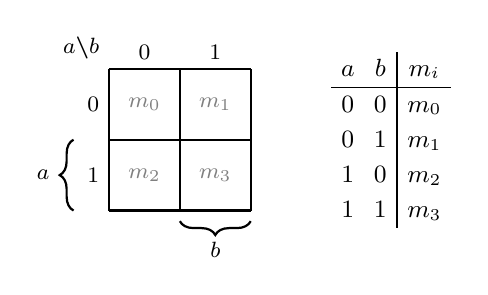
\begin{tikzpicture}[scale=0.9]
    % --- Karno haritası ---
    \draw[thick] (0,0) grid (2,2);
    \node[above, font=\footnotesize] at (0.5, 2) {0};
    \node[above, font=\footnotesize] at (1.5, 2) {1};
    \node[left, font=\footnotesize] at (0, 1.5) {0};
    \node[left, font=\footnotesize] at (0, 0.5) {1};
    \node[above left, font=\footnotesize\bfseries] at (0, 2) {$a$\textbackslash$b$};
    % Mini terim numaraları
    \node[font=\footnotesize, gray] at (0.5, 1.5) {$m_0$};
    \node[font=\footnotesize, gray] at (1.5, 1.5) {$m_1$};
    \node[font=\footnotesize, gray] at (0.5, 0.5) {$m_2$};
    \node[font=\footnotesize, gray] at (1.5, 0.5) {$m_3$};
    % Değişken bölge göstergeleri
    \draw[decorate, decoration={brace, amplitude=5pt}, thick] (-0.5, 0) -- (-0.5, 1) node[midway, left=5pt, font=\footnotesize] {$a$};
    \draw[decorate, decoration={brace, amplitude=5pt, mirror}, thick] (1, -0.15) -- (2, -0.15) node[midway, below=4pt, font=\footnotesize] {$b$};

    % --- Doğruluk tablosu ---
    \node[right, font=\small] at (3.0, 1.0) {
        \begin{tabular}{cc|c}
        $a$ & $b$ & $m_i$ \\
        \hline
        0 & 0 & $m_0$ \\
        0 & 1 & $m_1$ \\
        1 & 0 & $m_2$ \\
        1 & 1 & $m_3$ \\
        \end{tabular}
    };
\end{tikzpicture}
\caption{İki değişkenli Karno haritası ($a$, $b$) ve mini terim numaraları}
\label{fig:B.5}
\end{figure}

\begin{ornek}[B.4]
$F(a,b) = \Sigma(0, 3)$ fonksiyonunu Karno haritası ile sadeleştirin.

\textbf{Çözüm:}

Mini terimler haritaya yerleştirilir: $m_0$ ($a=0, b=0$) ve $m_3$ ($a=1, b=1$) hücrelerine 1 yazılır.

\begin{center}
\begin{tikzpicture}[scale=0.8]
    \draw[thick] (0,0) grid (2,2);
    \node[above, font=\footnotesize] at (0.5, 2) {0};
    \node[above, font=\footnotesize] at (1.5, 2) {1};
    \node[left, font=\footnotesize] at (0, 1.5) {0};
    \node[left, font=\footnotesize] at (0, 0.5) {1};
    \node[above left, font=\footnotesize\bfseries] at (0, 2) {$a$\textbackslash$b$};
    % Değerler
    \node at (0.5, 1.5) {1};
    \node at (1.5, 1.5) {0};
    \node at (0.5, 0.5) {0};
    \node at (1.5, 0.5) {1};
    % m0 ve m3 ayrı ayrı işaretlenir (gruplandırılamaz)
    \draw[rounded corners=2pt, very thick, sinyalkirmizi, opacity=0.8] (0.05,1.05) rectangle (0.95,1.95);
    \node[sinyalkirmizi, font=\footnotesize] (lab0) at (2.8, 1.5) {$\overline{a}\,\overline{b}$};
    \draw[thin, sinyalkirmizi, opacity=0.5] (0.95, 1.5) -- (lab0.west);
    \draw[rounded corners=2pt, very thick, sinyalmavi, opacity=0.8] (1.05,0.05) rectangle (1.95,0.95);
    \node[sinyalmavi, font=\footnotesize] (lab3) at (2.8, 0.5) {$a \cdot b$};
    \draw[thin, sinyalmavi, opacity=0.5] (1.95, 0.5) -- (lab3.west);
\end{tikzpicture}
\end{center}

$m_0$ ve $m_3$ köşegen konumdadır ve komşu değildir (iki bitte farklılaşır: hem $a$ hem $b$ değişir). Bu nedenle gruplandırılamazlar ve ifade sadeleştirilemez:
\[
F = \overline{a}\,\overline{b} + a \cdot b = a \odot b
\]
Bu, Dışlayan VEYA DEĞİL (eşitlik) fonksiyonudur: $a$ ve $b$ aynı değerdeyse çıkış 1 olur.
\end{ornek}

\subsubsection{Üç Değişkenli Karno Haritası}

Üç değişkenli bir fonksiyonun Karno haritası $2 \times 4 = 8$ hücreden oluşur. Satırlar $a$ değişkeninin değerlerini, sütunlar $bc$ çiftinin Gray kodu sırasıyla (00, 01, 11, 10) dizilmiş değerlerini temsil eder. Bu sıralama, komşu sütunların yalnızca tek bir bitte farklılaşmasını garanti eder. Ayrıca haritanın \textbf{sağ kenarı sol kenarına bitişik} sayılır: en sağdaki sütun (10) ile en soldaki sütun (00) yalnızca tek bir bitte farklılaştığından, bu iki sütundaki hücreler de komşudur. Gruplama yaparken bu kenar sarma göz önünde bulundurulmalıdır.

\begin{figure}[H]
\centering
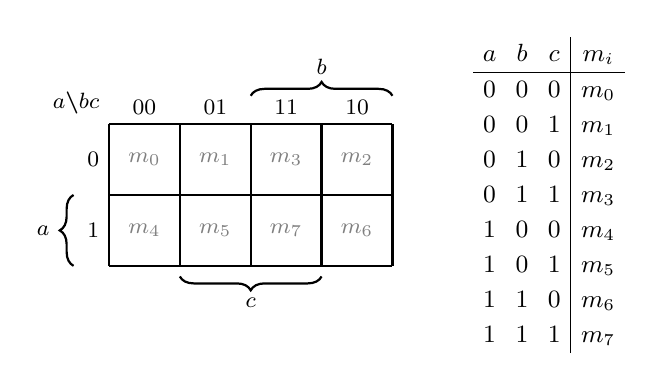
\begin{tikzpicture}[scale=0.9]
    % --- Karno haritası ---
    \draw[thick] (0,0) grid (4,2);
    \node[above, font=\footnotesize] at (0.5, 2) {00};
    \node[above, font=\footnotesize] at (1.5, 2) {01};
    \node[above, font=\footnotesize] at (2.5, 2) {11};
    \node[above, font=\footnotesize] at (3.5, 2) {10};
    \node[left, font=\footnotesize] at (0, 1.5) {0};
    \node[left, font=\footnotesize] at (0, 0.5) {1};
    \node[above left, font=\footnotesize\bfseries] at (0, 2) {$a$\textbackslash$bc$};
    % Mini terim numaraları (Gray kodu: sütunlar 00,01,11,10)
    % a=0 satırı: m0, m1, m3, m2
    \node[font=\footnotesize, gray] at (0.5, 1.5) {$m_0$};
    \node[font=\footnotesize, gray] at (1.5, 1.5) {$m_1$};
    \node[font=\footnotesize, gray] at (2.5, 1.5) {$m_3$};
    \node[font=\footnotesize, gray] at (3.5, 1.5) {$m_2$};
    % a=1 satırı: m4, m5, m7, m6
    \node[font=\footnotesize, gray] at (0.5, 0.5) {$m_4$};
    \node[font=\footnotesize, gray] at (1.5, 0.5) {$m_5$};
    \node[font=\footnotesize, gray] at (2.5, 0.5) {$m_7$};
    \node[font=\footnotesize, gray] at (3.5, 0.5) {$m_6$};
    % Değişken bölge göstergeleri
    \draw[decorate, decoration={brace, amplitude=5pt}, thick] (-0.5, 0) -- (-0.5, 1) node[midway, left=5pt, font=\footnotesize] {$a$};
    \draw[decorate, decoration={brace, amplitude=5pt}, thick] (2, 2.4) -- (4, 2.4) node[midway, above=4pt, font=\footnotesize] {$b$};
    \draw[decorate, decoration={brace, amplitude=5pt, mirror}, thick] (1, -0.15) -- (3, -0.15) node[midway, below=4pt, font=\footnotesize] {$c$};

    % --- Doğruluk tablosu ---
    \node[right, font=\small] at (5.0, 1.0) {
        \begin{tabular}{ccc|c}
        $a$ & $b$ & $c$ & $m_i$ \\
        \hline
        0 & 0 & 0 & $m_0$ \\
        0 & 0 & 1 & $m_1$ \\
        0 & 1 & 0 & $m_2$ \\
        0 & 1 & 1 & $m_3$ \\
        1 & 0 & 0 & $m_4$ \\
        1 & 0 & 1 & $m_5$ \\
        1 & 1 & 0 & $m_6$ \\
        1 & 1 & 1 & $m_7$ \\
        \end{tabular}
    };
\end{tikzpicture}
\caption{Üç değişkenli Karno haritası ve mini terim numaraları (sütunlar Gray kodu sırasıyla dizilir: 00, 01, 11, 10)}
\label{fig:B.6}
\end{figure}

\begin{ornek}[B.5]
$F = \overline{a}\,\overline{b}\,\overline{c} + a\,b\,c + a\,b\,\overline{c} + \overline{a}\,b\,\overline{c}$ fonksiyonunu Karno haritası ile sadeleştirin.

\textbf{Çözüm:}

Fonksiyondaki mini terimler Karno haritasına yerleştirilir ve komşu 1 değerleri gruplandırılır.

\begin{figure}[H]
\centering
\begin{tikzpicture}[scale=0.8]
    \draw (0,0) grid (4,2);
    \node[above, font=\footnotesize] at (0.5, 2) {00};
    \node[above, font=\footnotesize] at (1.5, 2) {01};
    \node[above, font=\footnotesize] at (2.5, 2) {11};
    \node[above, font=\footnotesize] at (3.5, 2) {10};
    \node[left, font=\footnotesize] at (0, 1.5) {0};
    \node[left, font=\footnotesize] at (0, 0.5) {1};
    \node[above left, font=\footnotesize] at (0, 2) {$a$\textbackslash $bc$};
    % Değişken bölge göstergeleri
    \draw[decorate, decoration={brace, amplitude=5pt}, thick] (-0.5, 0) -- (-0.5, 1) node[midway, left=5pt, font=\footnotesize] {$a$};
    \draw[decorate, decoration={brace, amplitude=5pt}, thick] (2, 2.4) -- (4, 2.4) node[midway, above=4pt, font=\footnotesize] {$b$};
    \draw[decorate, decoration={brace, amplitude=5pt, mirror}, thick] (1, -0.15) -- (3, -0.15) node[midway, below=4pt, font=\footnotesize] {$c$};
    % Hücre değerleri
    \node at (0.5,1.5) {1};
    \node at (1.5,1.5) {0};
    \node at (2.5,1.5) {0};
    \node at (3.5,1.5) {1};
    \node at (0.5,0.5) {0};
    \node at (1.5,0.5) {0};
    \node at (2.5,0.5) {1};
    \node at (3.5,0.5) {1};
    % Grup 1: {m6,m7} = a·b (kırmızı) — normal grup
    \draw[rounded corners=3pt, very thick, sinyalkirmizi, opacity=0.8] (2.05,0.05) rectangle (3.95,0.95);
    \node[sinyalkirmizi, font=\footnotesize] (lab1) at (5.2, 0.5) {$a \cdot b$};
    \draw[thin, sinyalkirmizi, opacity=0.5] (3.95, 0.5) -- (lab1.west);
    % Grup 2: {m0,m2} = a̅·c̅ (mavi - kenar sarma)
    % Sol parça: solu açık, sağı kapalı
    \draw[very thick, sinyalmavi, opacity=0.8]
        (-0.1,1.95) -- (0.95,1.95) -- (0.95,1.05) -- (-0.1,1.05);
    % Sağ parça: sağı açık, solu kapalı
    \draw[very thick, sinyalmavi, opacity=0.8]
        (4.1,1.95) -- (3.05,1.95) -- (3.05,1.05) -- (4.1,1.05);
    \node[sinyalmavi, font=\footnotesize] (lab2) at (5.2, 1.5) {$\overline{a}\,\overline{c}$};
    \draw[thin, sinyalmavi, opacity=0.5] (4.1, 1.7) -- (lab2.west);
\end{tikzpicture}
\caption*{Örnek B.5: $F$ fonksiyonunun Karno haritası ile sadeleştirilmesi}
\label{fig:B.7}
\end{figure}

$m_0$ yalnızca $\overline{a}\,\overline{c}$ grubu tarafından, $m_7$ ise yalnızca $a \cdot b$ grubu tarafından kapsandığından her iki grup da temel asal kapsayandır. Bu iki grup, dört 1 değerinin tamamını ($m_0$, $m_2$, $m_6$, $m_7$) kapsar; $\{m_2, m_6\}$ çifti ($b\overline{c}$) de geçerli bir grup olsa da her iki hücresi zaten kapsandığından gereksizdir.

Gruplandırma sonucunda:

\[
    F = a \cdot b + \overline{a} \cdot \overline{c}
\]
\end{ornek}

\subsubsection{Dört Değişkenli Karno Haritası}

Dört değişkenli harita $4 \times 4 = 16$ hücreden oluşur; hem satırlar ($ab$) hem sütunlar ($cd$) Gray kodu sırasıyla dizilir. Üç değişkenli haritada yalnızca sağ-sol kenarlar bitişikken, dört değişkenli haritada \textbf{hem sağ-sol hem üst-alt kenarlar birbirine bitişik} sayılır: harita bir torus (simit) gibi düşünülebilir. Dolayısıyla dört köşedeki hücreler de birbirine komşudur.

\begin{figure}[H]
\centering
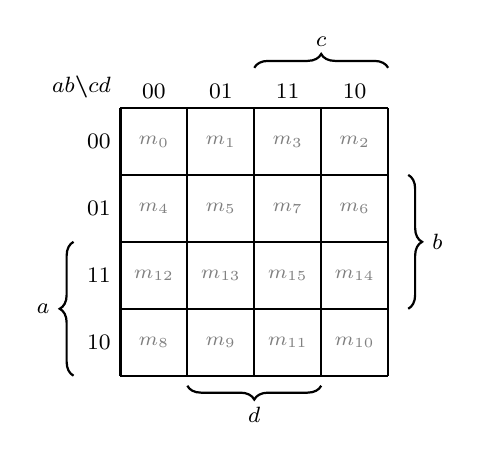
\begin{tikzpicture}[scale=0.85]
    % --- Karno haritası ---
    \draw[thick] (0,0) grid (4,4);
    \foreach \col/\lbl in {0/00, 1/01, 2/11, 3/10} {
        \node[above, font=\footnotesize] at (\col+0.5, 4) {\lbl};
    }
    \foreach \row/\lbl in {0/10, 1/11, 2/01, 3/00} {
        \node[left, font=\footnotesize] at (0, \row+0.5) {\lbl};
    }
    \node[above left, font=\footnotesize\bfseries] at (0, 4) {$ab$\textbackslash$cd$};
    % Mini terim numaraları
    \node[font=\scriptsize, gray] at (0.5, 3.5) {$m_0$};
    \node[font=\scriptsize, gray] at (1.5, 3.5) {$m_1$};
    \node[font=\scriptsize, gray] at (2.5, 3.5) {$m_3$};
    \node[font=\scriptsize, gray] at (3.5, 3.5) {$m_2$};
    \node[font=\scriptsize, gray] at (0.5, 2.5) {$m_4$};
    \node[font=\scriptsize, gray] at (1.5, 2.5) {$m_5$};
    \node[font=\scriptsize, gray] at (2.5, 2.5) {$m_7$};
    \node[font=\scriptsize, gray] at (3.5, 2.5) {$m_6$};
    \node[font=\scriptsize, gray] at (0.5, 1.5) {$m_{12}$};
    \node[font=\scriptsize, gray] at (1.5, 1.5) {$m_{13}$};
    \node[font=\scriptsize, gray] at (2.5, 1.5) {$m_{15}$};
    \node[font=\scriptsize, gray] at (3.5, 1.5) {$m_{14}$};
    \node[font=\scriptsize, gray] at (0.5, 0.5) {$m_8$};
    \node[font=\scriptsize, gray] at (1.5, 0.5) {$m_9$};
    \node[font=\scriptsize, gray] at (2.5, 0.5) {$m_{11}$};
    \node[font=\scriptsize, gray] at (3.5, 0.5) {$m_{10}$};
    % Değişken bölge göstergeleri (sol: a; sağ: b)
    \draw[decorate, decoration={brace, amplitude=5pt}, thick] (-0.7, 0) -- (-0.7, 2) node[midway, left=5pt, font=\footnotesize] {$a$};
    \draw[decorate, decoration={brace, amplitude=5pt, mirror}, thick] (4.3, 1) -- (4.3, 3) node[midway, right=5pt, font=\footnotesize] {$b$};
    % Değişken bölge göstergeleri (üst: c, alt: d)
    \draw[decorate, decoration={brace, amplitude=5pt}, thick] (2, 4.6) -- (4, 4.6) node[midway, above=4pt, font=\footnotesize] {$c$};
    \draw[decorate, decoration={brace, amplitude=5pt, mirror}, thick] (1, -0.15) -- (3, -0.15) node[midway, below=4pt, font=\footnotesize] {$d$};
\end{tikzpicture}
\caption{Dört değişkenli Karno haritası ve mini terim numaraları}
\label{fig:B.8}
\end{figure}

\begin{ornek}[B.6]
$F = \overline{a}\,b\,\overline{c} + \overline{a}\,\overline{c}\,d + a\,b\,\overline{c}\,\overline{d} + b\,c\,\overline{d}$ fonksiyonunu Karno haritası ile sadeleştirin.

\textbf{Çözüm:}

\begin{figure}[H]
\centering
\begin{tikzpicture}[scale=0.8]
    \draw (0,0) grid (4,4);
    \node[above, font=\footnotesize] at (0.5, 4) {00};
    \node[above, font=\footnotesize] at (1.5, 4) {01};
    \node[above, font=\footnotesize] at (2.5, 4) {11};
    \node[above, font=\footnotesize] at (3.5, 4) {10};
    \node[left, font=\footnotesize] at (0, 3.5) {00};
    \node[left, font=\footnotesize] at (0, 2.5) {01};
    \node[left, font=\footnotesize] at (0, 1.5) {11};
    \node[left, font=\footnotesize] at (0, 0.5) {10};
    \node[above left, font=\footnotesize] at (0, 4) {$ab$\textbackslash $cd$};
    % Değişken bölge göstergeleri (sol: a; sağ: b)
    \draw[decorate, decoration={brace, amplitude=5pt}, thick] (-0.7, 0) -- (-0.7, 2) node[midway, left=5pt, font=\footnotesize] {$a$};
    \draw[decorate, decoration={brace, amplitude=5pt, mirror}, thick] (4.5, 1) -- (4.5, 3) node[midway, right=5pt, font=\footnotesize] {$b$};
    % Değişken bölge göstergeleri (üst: c, alt: d)
    \draw[decorate, decoration={brace, amplitude=5pt}, thick] (2, 4.6) -- (4, 4.6) node[midway, above=4pt, font=\footnotesize] {$c$};
    \draw[decorate, decoration={brace, amplitude=5pt, mirror}, thick] (1, -0.15) -- (3, -0.15) node[midway, below=4pt, font=\footnotesize] {$d$};
    % Hücre değerleri
    % Row 00 (y=3.5): 0,1,0,0
    \node at (0.5,3.5) {0};
    \node at (1.5,3.5) {1};
    \node at (2.5,3.5) {0};
    \node at (3.5,3.5) {0};
    % Row 01 (y=2.5): 1,1,0,1
    \node at (0.5,2.5) {1};
    \node at (1.5,2.5) {1};
    \node at (2.5,2.5) {0};
    \node at (3.5,2.5) {1};
    % Row 11 (y=1.5): 1,0,0,1
    \node at (0.5,1.5) {1};
    \node at (1.5,1.5) {0};
    \node at (2.5,1.5) {0};
    \node at (3.5,1.5) {1};
    % Row 10 (y=0.5): 0,0,0,0
    \node at (0.5,0.5) {0};
    \node at (1.5,0.5) {0};
    \node at (2.5,0.5) {0};
    \node at (3.5,0.5) {0};
    % Grup 1: b·d̅ — {m4,m6,m12,m14} kenar sarma (kırmızı)
    % Sol parça: solu açık, sağı kapalı
    \draw[very thick, sinyalkirmizi, opacity=0.8]
        (-0.1,2.95) -- (0.95,2.95) -- (0.95,1.05) -- (-0.1,1.05);
    % Sağ parça: sağı açık, solu kapalı
    \draw[very thick, sinyalkirmizi, opacity=0.8]
        (4.1,2.95) -- (3.05,2.95) -- (3.05,1.05) -- (4.1,1.05);
    \node[sinyalkirmizi, font=\footnotesize] (lab1) at (5.5, 0.3) {$b\,\overline{d}$};
    \draw[thin, sinyalkirmizi, opacity=0.5] (4.1, 1.05) -- (lab1.west);
    % Grup 2: ā·c̅·d — {m1,m5} (mavi)
    \draw[rounded corners=3pt, very thick, sinyalmavi, opacity=0.8] (1.05,2.05) rectangle (1.95,3.95);
    \node[sinyalmavi, font=\footnotesize] (lab2) at (5.5, 4.3) {$\overline{a}\,\overline{c}\,d$};
    \draw[thin, sinyalmavi, opacity=0.5] (1.95, 3.95) -- (lab2.west);
\end{tikzpicture}
\caption*{Örnek B.6: $F$ fonksiyonunun 4 değişkenli Karno haritası ile sadeleştirilmesi}
\label{fig:B.9}
\end{figure}

Gruplandırma sonucunda:

\[
    F = b\,\overline{d} + \overline{a}\,\overline{c}\,d
\]
\end{ornek}

\subsubsection{Beş ve Altı Değişkenli Karno Haritaları}

Dört değişkenden fazlası için tek bir Karno haritası yeterli olmaz. Beş değişkenli fonksiyon iki adet $4 \times 4$ haritayla, altı değişkenli fonksiyon ise dört adet $4 \times 4$ haritayla gösterilir. Her harita beşinci (ve altıncı) değişkenin belirli bir değerine karşılık gelir. \textbf{Aynı konumdaki hücreler haritalar arasında komşu sayılır}; gruplama yapılırken bu komşuluk göz önünde bulundurulmalıdır. Aşağıdaki şekillerde haritalar üç boyutlu perspektifle gösterilmiştir; arka katmandaki hücreler ön katmandaki aynı konumdaki hücrelerle komşudur.

\begin{figure}[H]
\centering
\begin{tikzpicture}[scale=0.68, transform shape]
    % ====== Arka katman: a = 1 (mavi, sağa-yukarı kaydırılmış) ======
    \begin{scope}[shift={(2.0,1.5)}]
        \fill[blokmavi!8] (0,0) rectangle (4,4);
        \draw[thick, sinyalmavi!70] (0,0) grid (4,4);
        \foreach \col/\lbl in {0/00, 1/01, 2/11, 3/10} {
            \node[above, font=\footnotesize, sinyalmavi] at (\col+0.5, 4) {\lbl};
        }
        \foreach \row/\lbl in {0/10, 1/11, 2/01, 3/00} {
            \node[right, font=\footnotesize, sinyalmavi] at (4, \row+0.5) {\lbl};
        }
        \node[above, font=\small\bfseries, sinyalmavi] at (0.5, 4.5) {$a = 1$};
        % Mini terim numaraları
        \node[font=\tiny, sinyalmavi!60] at (0.5, 3.5) {$m_{16}$};
        \node[font=\tiny, sinyalmavi!60] at (1.5, 3.5) {$m_{17}$};
        \node[font=\tiny, sinyalmavi!60] at (2.5, 3.5) {$m_{19}$};
        \node[font=\tiny, sinyalmavi!60] at (3.5, 3.5) {$m_{18}$};
        \node[font=\tiny, sinyalmavi!60] at (0.5, 2.5) {$m_{20}$};
        \node[font=\tiny, sinyalmavi!60] at (1.5, 2.5) {$m_{21}$};
        \node[font=\tiny, sinyalmavi!60] at (2.5, 2.5) {$m_{23}$};
        \node[font=\tiny, sinyalmavi!60] at (3.5, 2.5) {$m_{22}$};
        \node[font=\tiny, sinyalmavi!60] at (0.5, 1.5) {$m_{28}$};
        \node[font=\tiny, sinyalmavi!60] at (1.5, 1.5) {$m_{29}$};
        \node[font=\tiny, sinyalmavi!60] at (2.5, 1.5) {$m_{31}$};
        \node[font=\tiny, sinyalmavi!60] at (3.5, 1.5) {$m_{30}$};
        \node[font=\tiny, sinyalmavi!60] at (0.5, 0.5) {$m_{24}$};
        \node[font=\tiny, sinyalmavi!60] at (1.5, 0.5) {$m_{25}$};
        \node[font=\tiny, sinyalmavi!60] at (2.5, 0.5) {$m_{27}$};
        \node[font=\tiny, sinyalmavi!60] at (3.5, 0.5) {$m_{26}$};
    \end{scope}

    % ====== Ön katman: a = 0 (siyah) ======
    \begin{scope}[shift={(0,0)}]
        \fill[white] (0,0) rectangle (4,4);
        \draw[thick] (0,0) grid (4,4);
        \foreach \col/\lbl in {0/00, 1/01, 2/11, 3/10} {
            \node[above, font=\footnotesize] at (\col+0.5, 4) {\lbl};
        }
        \foreach \row/\lbl in {0/10, 1/11, 2/01, 3/00} {
            \node[left, font=\footnotesize] at (0, \row+0.5) {\lbl};
        }
        \node[above left, font=\footnotesize\bfseries] at (0, 4) {$bc$\textbackslash$de$};
        \node[above, font=\small\bfseries] at (0.5, 4.5) {$a = 0$};
        % Mini terim numaraları
        \node[font=\tiny, gray] at (0.5, 3.5) {$m_0$};
        \node[font=\tiny, gray] at (1.5, 3.5) {$m_1$};
        \node[font=\tiny, gray] at (2.5, 3.5) {$m_3$};
        \node[font=\tiny, gray] at (3.5, 3.5) {$m_2$};
        \node[font=\tiny, gray] at (0.5, 2.5) {$m_4$};
        \node[font=\tiny, gray] at (1.5, 2.5) {$m_5$};
        \node[font=\tiny, gray] at (2.5, 2.5) {$m_7$};
        \node[font=\tiny, gray] at (3.5, 2.5) {$m_6$};
        \node[font=\tiny, gray] at (0.5, 1.5) {$m_{12}$};
        \node[font=\tiny, gray] at (1.5, 1.5) {$m_{13}$};
        \node[font=\tiny, gray] at (2.5, 1.5) {$m_{15}$};
        \node[font=\tiny, gray] at (3.5, 1.5) {$m_{14}$};
        \node[font=\tiny, gray] at (0.5, 0.5) {$m_8$};
        \node[font=\tiny, gray] at (1.5, 0.5) {$m_9$};
        \node[font=\tiny, gray] at (2.5, 0.5) {$m_{11}$};
        \node[font=\tiny, gray] at (3.5, 0.5) {$m_{10}$};
        % Değişken bölge göstergeleri (ön katmanda)
        \draw[decorate, decoration={brace, amplitude=5pt}, thick] (-0.7, 0) -- (-0.7, 2) node[midway, left=5pt, font=\footnotesize] {$b$};
        \draw[decorate, decoration={brace, amplitude=5pt, mirror}, thick] (1, -0.15) -- (3, -0.15) node[midway, below=4pt, font=\footnotesize] {$e$};
        \draw[decorate, decoration={brace, amplitude=5pt}, thick] (2, 4.7) -- (4, 4.7) node[midway, above=4pt, font=\footnotesize] {$d$};
        % d bölgesi arka katmanda da göster
        \node[font=\footnotesize, sinyalmavi] at (5.0, 6.8) {$d$};
        \draw[decorate, decoration={brace, amplitude=5pt}, thick, sinyalmavi] (4.0, 6.2) -- (6.0, 6.2);
    \end{scope}

    % ====== 3D bağlantı çizgileri (köşelerden köşelere — küp kenarları) ======
    % Dört köşe bağlantısı
    \draw[thin, gray, dashed] (4,4) -- (6.0,5.5);
    \draw[thin, gray, dashed] (4,0) -- (6.0,1.5);
    \draw[thin, gray, dashed] (0,0) -- (2.0,1.5);
    \draw[thin, gray, dashed] (0,4) -- (2.0,5.5);
    % Sol duvar (d bölgesi): ön sütun 01|11 sınırından arka katmana
    \draw[thin, gray, dashed] (2,4) -- (4.0,5.5);
    \draw[thin, gray, dashed] (2,0) -- (4.0,1.5);
    % Sol duvar ortası: ön satır 2 (b bölge sınırı) → arka katman
    \draw[thin, gray, dashed] (0,2) -- (2.0,3.5);
    % Sağ duvar: ön satır ortasından arka katmana (küpün sağ yüzü)
    \draw[thin, gray, dashed] (4,2) -- (6.0,3.5);  % satır 01|11 sınırı (orta)

    % c brace (arka katmanda, sağda — biraz daha sağa)
    \draw[decorate, decoration={brace, amplitude=5pt, mirror}, thick, sinyalmavi]
        (6.6, 2.5) -- (6.6, 4.5) node[midway, right=5pt, font=\footnotesize, sinyalmavi] {$c$};

    % ====================================================================
    % 2D AÇILIM (aynı şeklin sağ tarafında)
    % ====================================================================
    % a=0 haritası
    \begin{scope}[shift={(9,0)}]
        \draw[thick] (0,0) grid (4,4);
        \foreach \col/\lbl in {0/00, 1/01, 2/11, 3/10} {
            \node[above, font=\footnotesize] at (\col+0.5, 4) {\lbl};
        }
        \foreach \row/\lbl in {0/10, 1/11, 2/01, 3/00} {
            \node[left, font=\footnotesize] at (0, \row+0.5) {\lbl};
        }
        \node[above left, font=\footnotesize\bfseries] at (0, 4) {$bc$\textbackslash$de$};
        \node[above, font=\small\bfseries] at (2, 4.5) {$a = 0$};
        % Değerler
        \node at (0.5, 3.5) {0}; \node at (1.5, 3.5) {0};
        \node at (2.5, 3.5) {0}; \node[font=\bfseries] at (3.5, 3.5) {1};
        \node at (0.5, 2.5) {0}; \node at (1.5, 2.5) {0};
        \node[font=\bfseries] at (2.5, 2.5) {1}; \node[font=\bfseries] at (3.5, 2.5) {1};
        \node at (0.5, 1.5) {0}; \node at (1.5, 1.5) {0};
        \node[font=\bfseries] at (2.5, 1.5) {1}; \node[font=\bfseries] at (3.5, 1.5) {1};
        \node at (0.5, 0.5) {0}; \node at (1.5, 0.5) {0};
        \node at (2.5, 0.5) {0}; \node at (3.5, 0.5) {0};
        % Kırmızı grup: c·d
        \draw[rounded corners=3pt, very thick, sinyalkirmizi, opacity=0.8] (2.05,1.05) rectangle (3.95,2.95);
        % Yeşil: m2
        \draw[rounded corners=2pt, very thick, sinyalyesil, opacity=0.8] (3.05,3.05) rectangle (3.95,3.95);
    \end{scope}

    % a=1 haritası
    \begin{scope}[shift={(14.5,0)}]
        \draw[thick, sinyalmavi] (0,0) grid (4,4);
        \foreach \col/\lbl in {0/00, 1/01, 2/11, 3/10} {
            \node[above, font=\footnotesize, sinyalmavi] at (\col+0.5, 4) {\lbl};
        }
        \foreach \row/\lbl in {0/10, 1/11, 2/01, 3/00} {
            \node[right, font=\footnotesize, sinyalmavi] at (4, \row+0.5) {\lbl};
        }
        \node[above, font=\small\bfseries, sinyalmavi] at (2, 4.5) {$a = 1$};
        % Değerler
        \node at (0.5, 3.5) {0}; \node at (1.5, 3.5) {0};
        \node at (2.5, 3.5) {0}; \node[font=\bfseries, sinyalmavi] at (3.5, 3.5) {1};
        \node at (0.5, 2.5) {0}; \node at (1.5, 2.5) {0};
        \node[font=\bfseries, sinyalmavi] at (2.5, 2.5) {1}; \node[font=\bfseries, sinyalmavi] at (3.5, 2.5) {1};
        \node at (0.5, 1.5) {0}; \node at (1.5, 1.5) {0};
        \node[font=\bfseries, sinyalmavi] at (2.5, 1.5) {1}; \node[font=\bfseries, sinyalmavi] at (3.5, 1.5) {1};
        \node at (0.5, 0.5) {0}; \node at (1.5, 0.5) {0};
        \node at (2.5, 0.5) {0}; \node at (3.5, 0.5) {0};
        % Kırmızı grup: c·d
        \draw[rounded corners=3pt, very thick, sinyalkirmizi, opacity=0.8] (2.05,1.05) rectangle (3.95,2.95);
        % Yeşil: m18
        \draw[rounded corners=2pt, very thick, sinyalyesil, opacity=0.8] (3.05,3.05) rectangle (3.95,3.95);
    \end{scope}

    % Katmanlar arası oklar ve etiketler (iki harita arasındaki boşlukta)
    \draw[<->, very thick, sinyalkirmizi] (12.95, 2.0) -- (16.55, 2.0);
    \node[sinyalkirmizi, font=\small, fill=white, inner sep=1pt] at (13.75, 2.4) {$c \cdot d$};
    \draw[<->, thick, sinyalyesil] (12.95, 3.5) -- (17.55, 3.5);
    \node[sinyalyesil, font=\small, fill=white, inner sep=1pt] at (13.75, 3.9) {$\overline{b}\,\overline{c}\,d\,\overline{e}$};

\end{tikzpicture}
\caption{Beş değişkenli Karno haritası (sol: 3D görünüm, sağ: 2D açılım ve gruplama örneği, $F = \Sigma(2,6,7,14,15,18,22,23,30,31)$)}
\label{fig:B.karno5}
\end{figure}

Şekil~\ref{fig:B.karno5}'in sağ tarafındaki 2D açılımda iki tür gruplama görülmektedir:

\begin{itemize}[nosep]
    \item \textbf{Her iki katmanda ortak grup} (kırmızı): $a=0$ katmanındaki $\{m_6, m_7, m_{14}, m_{15}\}$ ve $a=1$ katmanındaki $\{m_{22}, m_{23}, m_{30}, m_{31}\}$ hücreleri aynı konumdadır ve hepsi 1 değerini taşır. Sekiz hücrelik bu grup $a$ değişkenini de eler ve sonuç yalnızca $c \cdot d$ olur.
    \item \textbf{Katmanlar arası ikili grup} (yeşil): $m_2$ ($a=0$, $bc{=}00$, $de{=}10$) ile $m_{18}$ ($a=1$, aynı konum) komşudur. İkisi arasında yalnızca $a$ değişkeni farklılaştığından bu ikili grubun sonucu $\overline{b}\,\overline{c}\,d\,\overline{e}$ olur.
\end{itemize}

\noindent Sonuç: $F = c \cdot d + \overline{b}\,\overline{c}\,d\,\overline{e}$.

\begin{figure}[H]
\centering
\begin{tikzpicture}[scale=0.65, transform shape]
    % ============================================================
    % SOL TARAF: 3D GÖRÜNÜM (sola kaydırılmış)
    % ============================================================
    \begin{scope}[shift={(-2,0)}]
    % Katman 4 (en arka): ab=10 — turuncu
    \begin{scope}[shift={(4.8,3.6)}]
        \fill[brown!10] (0,0) rectangle (4,4);
        \draw[thick, brown!50!black] (0,0) grid (4,4);
        \node[above, font=\small\bfseries, brown!70!black] at (0.8, 4.3) {$ab = 10$};
        % Mini terim numaraları (ab=10)
        \node[font=\tiny, brown!50!black] at (0.5, 3.5) {$m_{32}$};
        \node[font=\tiny, brown!50!black] at (1.5, 3.5) {$m_{33}$};
        \node[font=\tiny, brown!50!black] at (2.5, 3.5) {$m_{35}$};
        \node[font=\tiny, brown!50!black] at (3.5, 3.5) {$m_{34}$};
        \node[font=\tiny, brown!50!black] at (0.5, 2.5) {$m_{36}$};
        \node[font=\tiny, brown!50!black] at (1.5, 2.5) {$m_{37}$};
        \node[font=\tiny, brown!50!black] at (2.5, 2.5) {$m_{39}$};
        \node[font=\tiny, brown!50!black] at (3.5, 2.5) {$m_{38}$};
        \node[font=\tiny, brown!50!black] at (0.5, 1.5) {$m_{44}$};
        \node[font=\tiny, brown!50!black] at (1.5, 1.5) {$m_{45}$};
        \node[font=\tiny, brown!50!black] at (2.5, 1.5) {$m_{47}$};
        \node[font=\tiny, brown!50!black] at (3.5, 1.5) {$m_{46}$};
        \node[font=\tiny, brown!50!black] at (0.5, 0.5) {$m_{40}$};
        \node[font=\tiny, brown!50!black] at (1.5, 0.5) {$m_{41}$};
        \node[font=\tiny, brown!50!black] at (2.5, 0.5) {$m_{43}$};
        \node[font=\tiny, brown!50!black] at (3.5, 0.5) {$m_{42}$};
    \end{scope}
    % Katman 3: ab=11 — yeşil (daha koyu)
    \begin{scope}[shift={(3.2,2.4)}]
        \fill[blokyesil!15] (0,0) rectangle (4,4);
        \draw[thick, sinyalyesil!80] (0,0) grid (4,4);
        \node[above, font=\small\bfseries, sinyalyesil!90!black] at (0.8, 4.3) {$ab = 11$};
        % Mini terim numaraları (ab=11)
        \node[font=\tiny, sinyalyesil!50] at (0.5, 3.5) {$m_{48}$};
        \node[font=\tiny, sinyalyesil!50] at (1.5, 3.5) {$m_{49}$};
        \node[font=\tiny, sinyalyesil!50] at (2.5, 3.5) {$m_{51}$};
        \node[font=\tiny, sinyalyesil!50] at (3.5, 3.5) {$m_{50}$};
        \node[font=\tiny, sinyalyesil!50] at (0.5, 2.5) {$m_{52}$};
        \node[font=\tiny, sinyalyesil!50] at (1.5, 2.5) {$m_{53}$};
        \node[font=\tiny, sinyalyesil!50] at (2.5, 2.5) {$m_{55}$};
        \node[font=\tiny, sinyalyesil!50] at (3.5, 2.5) {$m_{54}$};
        \node[font=\tiny, sinyalyesil!50] at (0.5, 1.5) {$m_{60}$};
        \node[font=\tiny, sinyalyesil!50] at (1.5, 1.5) {$m_{61}$};
        \node[font=\tiny, sinyalyesil!50] at (2.5, 1.5) {$m_{63}$};
        \node[font=\tiny, sinyalyesil!50] at (3.5, 1.5) {$m_{62}$};
        \node[font=\tiny, sinyalyesil!50] at (0.5, 0.5) {$m_{56}$};
        \node[font=\tiny, sinyalyesil!50] at (1.5, 0.5) {$m_{57}$};
        \node[font=\tiny, sinyalyesil!50] at (2.5, 0.5) {$m_{59}$};
        \node[font=\tiny, sinyalyesil!50] at (3.5, 0.5) {$m_{58}$};
    \end{scope}
    % Katman 2: ab=01 — mavi
    \begin{scope}[shift={(1.6,1.2)}]
        \fill[blokmavi!10] (0,0) rectangle (4,4);
        \draw[thick, sinyalmavi!60] (0,0) grid (4,4);
        \node[above, font=\small\bfseries, sinyalmavi!80!black] at (0.8, 4.3) {$ab = 01$};
        % Mini terim numaraları (ab=01)
        \node[font=\tiny, sinyalmavi!50] at (0.5, 3.5) {$m_{16}$};
        \node[font=\tiny, sinyalmavi!50] at (1.5, 3.5) {$m_{17}$};
        \node[font=\tiny, sinyalmavi!50] at (2.5, 3.5) {$m_{19}$};
        \node[font=\tiny, sinyalmavi!50] at (3.5, 3.5) {$m_{18}$};
        \node[font=\tiny, sinyalmavi!50] at (0.5, 2.5) {$m_{20}$};
        \node[font=\tiny, sinyalmavi!50] at (1.5, 2.5) {$m_{21}$};
        \node[font=\tiny, sinyalmavi!50] at (2.5, 2.5) {$m_{23}$};
        \node[font=\tiny, sinyalmavi!50] at (3.5, 2.5) {$m_{22}$};
        \node[font=\tiny, sinyalmavi!50] at (0.5, 1.5) {$m_{28}$};
        \node[font=\tiny, sinyalmavi!50] at (1.5, 1.5) {$m_{29}$};
        \node[font=\tiny, sinyalmavi!50] at (2.5, 1.5) {$m_{31}$};
        \node[font=\tiny, sinyalmavi!50] at (3.5, 1.5) {$m_{30}$};
        \node[font=\tiny, sinyalmavi!50] at (0.5, 0.5) {$m_{24}$};
        \node[font=\tiny, sinyalmavi!50] at (1.5, 0.5) {$m_{25}$};
        \node[font=\tiny, sinyalmavi!50] at (2.5, 0.5) {$m_{27}$};
        \node[font=\tiny, sinyalmavi!50] at (3.5, 0.5) {$m_{26}$};
    \end{scope}
    % Katman 1 (en ön): ab=00 — siyah
    \begin{scope}[shift={(0,0)}]
        \fill[white] (0,0) rectangle (4,4);
        \draw[thick] (0,0) grid (4,4);
        \foreach \col/\lbl in {0/00, 1/01, 2/11, 3/10} {
            \node[above, font=\footnotesize] at (\col+0.5, 4) {\lbl};
        }
        \foreach \row/\lbl in {0/10, 1/11, 2/01, 3/00} {
            \node[left, font=\footnotesize] at (0, \row+0.5) {\lbl};
        }
        \node[above left, font=\footnotesize\bfseries] at (0, 4) {$cd$\textbackslash$ef$};
        \node[above, font=\small\bfseries] at (0.8, 4.3) {$ab = 00$};
        % Mini terim numaraları (ab=00, cdabef sırasıyla)
        % cd=00: ef=00→m0, 01→m1, 11→m3, 10→m2
        \node[font=\tiny, gray] at (0.5, 3.5) {$m_0$};
        \node[font=\tiny, gray] at (1.5, 3.5) {$m_1$};
        \node[font=\tiny, gray] at (2.5, 3.5) {$m_3$};
        \node[font=\tiny, gray] at (3.5, 3.5) {$m_2$};
        % cd=01
        \node[font=\tiny, gray] at (0.5, 2.5) {$m_4$};
        \node[font=\tiny, gray] at (1.5, 2.5) {$m_5$};
        \node[font=\tiny, gray] at (2.5, 2.5) {$m_7$};
        \node[font=\tiny, gray] at (3.5, 2.5) {$m_6$};
        % cd=11
        \node[font=\tiny, gray] at (0.5, 1.5) {$m_{12}$};
        \node[font=\tiny, gray] at (1.5, 1.5) {$m_{13}$};
        \node[font=\tiny, gray] at (2.5, 1.5) {$m_{15}$};
        \node[font=\tiny, gray] at (3.5, 1.5) {$m_{14}$};
        % cd=10
        \node[font=\tiny, gray] at (0.5, 0.5) {$m_8$};
        \node[font=\tiny, gray] at (1.5, 0.5) {$m_9$};
        \node[font=\tiny, gray] at (2.5, 0.5) {$m_{11}$};
        \node[font=\tiny, gray] at (3.5, 0.5) {$m_{10}$};
        % Değişken bölge göstergeleri (ön katmanda)
        \draw[decorate, decoration={brace, amplitude=5pt}, thick] (-0.7, 0) -- (-0.7, 2) node[midway, left=5pt, font=\footnotesize] {$c$};
        \draw[decorate, decoration={brace, amplitude=5pt, mirror}, thick] (4.3, 1) -- (4.3, 3) node[midway, right=5pt, font=\footnotesize] {$d$};
        \draw[decorate, decoration={brace, amplitude=5pt}, thick] (2, 4.7) -- (4, 4.7) node[midway, above=4pt, font=\footnotesize] {$e$};
        \draw[decorate, decoration={brace, amplitude=5pt, mirror}, thick] (1, -0.15) -- (3, -0.15) node[midway, below=4pt, font=\footnotesize] {$f$};
    \end{scope}
    % d ve e brace'leri (arka katmanda, brown renkte)
    \draw[decorate, decoration={brace, amplitude=5pt, mirror}, thick, brown!70!black]
        (9.0, 4.6) -- (9.0, 6.6) node[midway, right=5pt, font=\footnotesize, brown!70!black] {$d$};
    \draw[decorate, decoration={brace, amplitude=5pt}, thick, brown!70!black]
        (6.8, 7.9) -- (8.8, 7.9) node[midway, above=4pt, font=\footnotesize, brown!70!black] {$e$};
    % 3D bağlantı çizgileri (küp kenarları)
    \draw[thin, gray!60, dashed] (0,4) -- (4.8,7.6);
    \draw[thin, gray!60, dashed] (4,4) -- (8.8,7.6);
    \draw[thin, gray!60, dashed] (4,0) -- (8.8,3.6);
    \draw[thin, gray!60, dashed] (0,0) -- (4.8,3.6);
    % İç kesikli çizgiler (küp yüzleri — biraz daha soluk)
    \draw[thin, gray!40, dashed] (2,4) -- (6.8,7.6);
    \draw[thin, gray!40, dashed] (2,0) -- (6.8,3.6);
    \draw[thin, gray!40, dashed] (0,2) -- (4.8,5.6);
    \draw[thin, gray!40, dashed] (4,2) -- (8.8,5.6);
    % a brace: yeşil+kahverengi katmanların (ab=11,ab=10) sol üst köşesi
    % ab=11 sol üst: (3.2, 6.4), ab=10 sol üst: (4.8, 7.6)
    \draw[decorate, decoration={brace, amplitude=4pt}, thick]
        (3.0, 6.6) -- (4.6, 7.8) node[midway, above left=2pt, font=\footnotesize] {$a$};
    % b brace: mavi+yeşil katmanların (ab=01,ab=11) sağ alt köşesi
    % ab=01 sağ alt: (5.6, 1.2), ab=11 sağ alt: (7.2, 2.4)
    \draw[decorate, decoration={brace, amplitude=4pt, mirror}, thick]
        (5.8, 1.0) -- (7.4, 2.2) node[midway, below right=2pt, font=\footnotesize] {$b$};
    \end{scope} % sol taraf scope sonu

    % ============================================================
    % SAĞ TARAF: 2D AÇILIM (2×2 düzen, sağa kaydırılmış)
    % ============================================================
    \def\dx{10}  % sol üst haritanın x ofseti
    \def\hgap{5.5} % haritalar arası yatay boşluk
    \def\vgap{5.5} % haritalar arası dikey boşluk

    % ab=00 (sol üst)
    \begin{scope}[shift={(\dx, \vgap)}]
        \draw[thick] (0,0) grid (4,4);
        \foreach \col/\lbl in {0/00, 1/01, 2/11, 3/10} {
            \node[above, font=\footnotesize] at (\col+0.5, 4) {\lbl};
        }
        \foreach \row/\lbl in {0/10, 1/11, 2/01, 3/00} {
            \node[left, font=\footnotesize] at (0, \row+0.5) {\lbl};
        }
        \node[above left, font=\footnotesize\bfseries] at (0, 4) {$cd$\textbackslash$ef$};
        \node[above right, font=\small\bfseries] at (0, 4.4) {$ab = 00$};
        % Mini terimler (abcdef: ab=00, cd=satır Gray, ef=sütun Gray)
        \node[font=\tiny, gray] at (0.5, 3.5) {0}; \node[font=\tiny, gray] at (1.5, 3.5) {1};
        \node[font=\tiny, gray] at (2.5, 3.5) {3}; \node[font=\tiny, gray] at (3.5, 3.5) {2};
        \node[font=\tiny, gray] at (0.5, 2.5) {4}; \node[font=\tiny, gray] at (1.5, 2.5) {5};
        \node[font=\tiny, gray] at (2.5, 2.5) {7}; \node[font=\tiny, gray] at (3.5, 2.5) {6};
        \node[font=\tiny, gray] at (0.5, 1.5) {12}; \node[font=\tiny, gray] at (1.5, 1.5) {13};
        \node[font=\tiny, gray] at (2.5, 1.5) {15}; \node[font=\tiny, gray] at (3.5, 1.5) {14};
        \node[font=\tiny, gray] at (0.5, 0.5) {8}; \node[font=\tiny, gray] at (1.5, 0.5) {9};
        \node[font=\tiny, gray] at (2.5, 0.5) {11}; \node[font=\tiny, gray] at (3.5, 0.5) {10};
    \end{scope}

    % ab=01 (sağ üst, mavi)
    \begin{scope}[shift={(\dx+\hgap, \vgap)}]
        \draw[thick, sinyalmavi] (0,0) grid (4,4);
        \foreach \col/\lbl in {0/00, 1/01, 2/11, 3/10} {
            \node[above, font=\footnotesize, sinyalmavi] at (\col+0.5, 4) {\lbl};
        }
        \foreach \row/\lbl in {0/10, 1/11, 2/01, 3/00} {
            \node[right, font=\footnotesize, sinyalmavi] at (4, \row+0.5) {\lbl};
        }
        \node[above right, font=\small\bfseries, sinyalmavi] at (0, 4.4) {$ab = 01$};
        % Mini terimler (ab=01)
        \node[font=\tiny, sinyalmavi!70] at (0.5, 3.5) {16}; \node[font=\tiny, sinyalmavi!70] at (1.5, 3.5) {17};
        \node[font=\tiny, sinyalmavi!70] at (2.5, 3.5) {19}; \node[font=\tiny, sinyalmavi!70] at (3.5, 3.5) {18};
        \node[font=\tiny, sinyalmavi!70] at (0.5, 2.5) {20}; \node[font=\tiny, sinyalmavi!70] at (1.5, 2.5) {21};
        \node[font=\tiny, sinyalmavi!70] at (2.5, 2.5) {23}; \node[font=\tiny, sinyalmavi!70] at (3.5, 2.5) {22};
        \node[font=\tiny, sinyalmavi!70] at (0.5, 1.5) {28}; \node[font=\tiny, sinyalmavi!70] at (1.5, 1.5) {29};
        \node[font=\tiny, sinyalmavi!70] at (2.5, 1.5) {31}; \node[font=\tiny, sinyalmavi!70] at (3.5, 1.5) {30};
        \node[font=\tiny, sinyalmavi!70] at (0.5, 0.5) {24}; \node[font=\tiny, sinyalmavi!70] at (1.5, 0.5) {25};
        \node[font=\tiny, sinyalmavi!70] at (2.5, 0.5) {27}; \node[font=\tiny, sinyalmavi!70] at (3.5, 0.5) {26};
    \end{scope}

    % ab=10 (sol alt, turuncu)
    \begin{scope}[shift={(\dx, 0)}]
        \draw[thick, brown!60!black] (0,0) grid (4,4);
        \foreach \col/\lbl in {0/00, 1/01, 2/11, 3/10} {
            \node[below, font=\footnotesize, brown!70!black] at (\col+0.5, 0) {\lbl};
        }
        \foreach \row/\lbl in {0/10, 1/11, 2/01, 3/00} {
            \node[left, font=\footnotesize, brown!70!black] at (0, \row+0.5) {\lbl};
        }
        \node[below left, font=\footnotesize\bfseries, brown!70!black] at (0, 0) {$cd$\textbackslash$ef$};
        \node[above right, font=\small\bfseries, brown!70!black] at (0, 4.4) {$ab = 10$};
        % Mini terimler (ab=10)
        \node[font=\tiny, brown!60!black] at (0.5, 3.5) {32}; \node[font=\tiny, brown!60!black] at (1.5, 3.5) {33};
        \node[font=\tiny, brown!60!black] at (2.5, 3.5) {35}; \node[font=\tiny, brown!60!black] at (3.5, 3.5) {34};
        \node[font=\tiny, brown!60!black] at (0.5, 2.5) {36}; \node[font=\tiny, brown!60!black] at (1.5, 2.5) {37};
        \node[font=\tiny, brown!60!black] at (2.5, 2.5) {39}; \node[font=\tiny, brown!60!black] at (3.5, 2.5) {38};
        \node[font=\tiny, brown!60!black] at (0.5, 1.5) {44}; \node[font=\tiny, brown!60!black] at (1.5, 1.5) {45};
        \node[font=\tiny, brown!60!black] at (2.5, 1.5) {47}; \node[font=\tiny, brown!60!black] at (3.5, 1.5) {46};
        \node[font=\tiny, brown!60!black] at (0.5, 0.5) {40}; \node[font=\tiny, brown!60!black] at (1.5, 0.5) {41};
        \node[font=\tiny, brown!60!black] at (2.5, 0.5) {43}; \node[font=\tiny, brown!60!black] at (3.5, 0.5) {42};
    \end{scope}

    % ab=11 (sağ alt, yeşil — daha koyu)
    \begin{scope}[shift={(\dx+\hgap, 0)}]
        \draw[thick, sinyalyesil!90!black] (0,0) grid (4,4);
        \foreach \col/\lbl in {0/00, 1/01, 2/11, 3/10} {
            \node[below, font=\footnotesize, sinyalyesil!90!black] at (\col+0.5, 0) {\lbl};
        }
        \foreach \row/\lbl in {0/10, 1/11, 2/01, 3/00} {
            \node[right, font=\footnotesize, sinyalyesil!90!black] at (4, \row+0.5) {\lbl};
        }
        \node[above right, font=\small\bfseries, sinyalyesil!90!black] at (0, 4.4) {$ab = 11$};
        % Mini terimler (ab=11)
        \node[font=\tiny, sinyalyesil!80!black] at (0.5, 3.5) {48}; \node[font=\tiny, sinyalyesil!80!black] at (1.5, 3.5) {49};
        \node[font=\tiny, sinyalyesil!80!black] at (2.5, 3.5) {51}; \node[font=\tiny, sinyalyesil!80!black] at (3.5, 3.5) {50};
        \node[font=\tiny, sinyalyesil!80!black] at (0.5, 2.5) {52}; \node[font=\tiny, sinyalyesil!80!black] at (1.5, 2.5) {53};
        \node[font=\tiny, sinyalyesil!80!black] at (2.5, 2.5) {55}; \node[font=\tiny, sinyalyesil!80!black] at (3.5, 2.5) {54};
        \node[font=\tiny, sinyalyesil!80!black] at (0.5, 1.5) {60}; \node[font=\tiny, sinyalyesil!80!black] at (1.5, 1.5) {61};
        \node[font=\tiny, sinyalyesil!80!black] at (2.5, 1.5) {63}; \node[font=\tiny, sinyalyesil!80!black] at (3.5, 1.5) {62};
        \node[font=\tiny, sinyalyesil!80!black] at (0.5, 0.5) {56}; \node[font=\tiny, sinyalyesil!80!black] at (1.5, 0.5) {57};
        \node[font=\tiny, sinyalyesil!80!black] at (2.5, 0.5) {59}; \node[font=\tiny, sinyalyesil!80!black] at (3.5, 0.5) {58};
    \end{scope}

    % Komşuluk okları (2D düzende — haritalar arası boşluğun ortasında)
    \draw[<->, very thick, sinyalkirmizi] (\dx+4.15, 7.5) -- (\dx+\hgap-0.15, 7.5)
        node[midway, above, font=\scriptsize] {komşu};
    \draw[<->, very thick, sinyalkirmizi] (\dx+4.15, 2) -- (\dx+\hgap-0.15, 2)
        node[midway, above, font=\scriptsize] {komşu};
    \draw[<->, very thick, sinyalkirmizi] (\dx+2, \vgap-0.15) -- (\dx+2, \vgap-1.35)
        node[midway, right, font=\scriptsize] {komşu};
    \draw[<->, very thick, sinyalkirmizi] (\dx+\hgap+2, \vgap-0.15) -- (\dx+\hgap+2, \vgap-1.35)
        node[midway, right, font=\scriptsize] {komşu};

    % Değişken bölge parantezleri (2D düzende)
    \draw[decorate, decoration={brace, amplitude=5pt}, thick] (\dx-0.7, \vgap) -- (\dx-0.7, \vgap+2)
        node[midway, left=5pt, font=\footnotesize] {$c$};
    \draw[decorate, decoration={brace, amplitude=5pt}, thick] (\dx+2, \vgap+4.7) -- (\dx+4, \vgap+4.7)
        node[midway, above=4pt, font=\footnotesize] {$e$};
    \draw[decorate, decoration={brace, amplitude=5pt, mirror}, thick]
        (\dx+\hgap+4.7, \vgap+1) -- (\dx+\hgap+4.7, \vgap+3)
        node[midway, right=5pt, font=\footnotesize] {$d$};
    \draw[decorate, decoration={brace, amplitude=5pt, mirror}, thick]
        (\dx+1, -0.6) -- (\dx+3, -0.6)
        node[midway, below=4pt, font=\footnotesize] {$f$};
    % a ve b parantezleri (harita düzenini kapsar)
    \draw[decorate, decoration={brace, amplitude=6pt, mirror}, thick]
        (\dx+\hgap, -1.0) -- (\dx+\hgap+4, -1.0)
        node[midway, below=6pt, font=\footnotesize] {$b$};
    \draw[decorate, decoration={brace, amplitude=6pt}, thick]
        (\dx-1.2, 0) -- (\dx-1.2, 4)
        node[midway, left=6pt, font=\footnotesize] {$a$};

\end{tikzpicture}
\caption{Altı değişkenli Karno haritası (sol: 3D görünüm, sağ: 2D açılım, $2 \times 2$ düzen). Komşu haritalar arasındaki aynı konumdaki hücreler de komşudur.}
\label{fig:B.karno6}
\end{figure}

Değişken sayısı arttıkça Karno haritası hızla karmaşıklaşır ve elle çözüm zorlaşır. Yedi ve üzeri değişken için üç boyutlu gösterim bile olanaklı değildir. Bu nedenle beşten fazla değişkenli fonksiyonlar için bir sonraki alt bölümde tanıtılacak Quine--McCluskey algoritması tercih edilir.

\subsection{Önemsenmeyen Durumlar}

Bazı giriş kombinasyonları uygulamada hiçbir zaman gerçekleşmez ya da gerçekleşse bile çıkışın ne olduğu önemsizdir. Bu durumlar doğruluk tablosunda ve Karno haritasında ``X'' ile gösterilir ve \textbf{önemsenmeyen durum} (İngilizcesi: \textit{don't care}) olarak adlandırılır.

Önemsenmeyen durumlar, Karno haritasında gruplamayı büyütmek için hem 1 hem de 0 olarak ele alınabilir. Bu esneklik, daha büyük gruplar oluşturulmasına ve dolayısıyla daha sadeleştirilmiş ifadelerin elde edilmesine olanak tanır. Tasarımcı, her X hücresini gruplama sırasında 1 veya 0 olarak serbestçe seçer; hangisi daha büyük bir grup oluşturuyorsa o tercih edilir.

Önemsenmeyen durumlar özellikle denetim birimi tasarımlarında sıkça karşılaşılır; çünkü buyruğun işlem kodu alanındaki bazı bit kombinasyonları geçerli bir buyrukla eşleşmez (bu ekin ilerleyen bölümlerinde bunun bir örneği verilecektir).

\begin{ornek}[B.7]
Bir BCD (ikilik Kodlanmış Onluk) -- sayısal gösterimde yalnızca 0000'dan 1001'e kadar olan kombinasyonlar geçerlidir (onluk 0--9). $F(a,b,c,d) = \Sigma(1, 3, 5, 7, 9)$ fonksiyonunu, geçersiz BCD kombinasyonlarını ($m_{10}$--$m_{15}$) önemsenmeyen durum olarak kullanarak sadeleştirin.

\textbf{Çözüm:}

Önemsenmeyen durumlar: $d = \{10, 11, 12, 13, 14, 15\}$.

\begin{center}
\begin{tikzpicture}[scale=0.8]
    \draw[thick] (0,0) grid (4,4);
    \foreach \col/\lbl in {0/00, 1/01, 2/11, 3/10} {
        \node[above, font=\footnotesize] at (\col+0.5, 4) {\lbl};
    }
    \foreach \row/\lbl in {0/10, 1/11, 2/01, 3/00} {
        \node[left, font=\footnotesize] at (0, \row+0.5) {\lbl};
    }
    \node[above left, font=\footnotesize] at (0, 4) {$ab$\textbackslash $cd$};
    % Değişken bölge göstergeleri (sol: a; sağ: b)
    \draw[decorate, decoration={brace, amplitude=5pt}, thick] (-0.7, 0) -- (-0.7, 2) node[midway, left=5pt, font=\footnotesize] {$a$};
    \draw[decorate, decoration={brace, amplitude=5pt, mirror}, thick] (4.5, 1) -- (4.5, 3) node[midway, right=5pt, font=\footnotesize] {$b$};
    % Değişken bölge göstergeleri (üst: c, alt: d)
    \draw[decorate, decoration={brace, amplitude=5pt}, thick] (2, 4.6) -- (4, 4.6) node[midway, above=4pt, font=\footnotesize] {$c$};
    \draw[decorate, decoration={brace, amplitude=5pt, mirror}, thick] (1, -0.15) -- (3, -0.15) node[midway, below=4pt, font=\footnotesize] {$d$};
    % Hücre değerleri — BCD: 0-9 geçerli, 10-15 önemsenmeyen
    % ab=00: cd=00(m0)→0, 01(m1)→1, 11(m3)→1, 10(m2)→0
    \node at (0.5,3.5) {0};
    \node at (1.5,3.5) {1};
    \node at (2.5,3.5) {1};
    \node at (3.5,3.5) {0};
    % ab=01: cd=00(m4)→0, 01(m5)→1, 11(m7)→1, 10(m6)→0
    \node at (0.5,2.5) {0};
    \node at (1.5,2.5) {1};
    \node at (2.5,2.5) {1};
    \node at (3.5,2.5) {0};
    % ab=11: cd=00(m12)→X, 01(m13)→X, 11(m15)→X, 10(m14)→X
    \node[sinyalkirmizi] at (0.5,1.5) {X};
    \node[sinyalkirmizi] at (1.5,1.5) {X};
    \node[sinyalkirmizi] at (2.5,1.5) {X};
    \node[sinyalkirmizi] at (3.5,1.5) {X};
    % ab=10: cd=00(m8)→0, 01(m9)→1, 11(m11)→X, 10(m10)→X
    \node at (0.5,0.5) {0};
    \node at (1.5,0.5) {1};
    \node[sinyalkirmizi] at (2.5,0.5) {X};
    \node[sinyalkirmizi] at (3.5,0.5) {X};
    % Gruplama: w=1 olan tüm hücreler (sütun 01 ve 11) — X'leri de kullanarak
    \draw[rounded corners=3pt, very thick, sinyalmavi, opacity=0.8] (0.95,0.05) rectangle (2.95,3.95);
    % Grup sonuç etiketi
    \node[sinyalmavi, font=\footnotesize] (labD) at (5.0, 2.0) {$d$};
    \draw[thin, sinyalmavi, opacity=0.5] (2.95, 2.0) -- (labD.west);
\end{tikzpicture}
\end{center}

Önemsenmeyen durumlar (X) gruplama sırasında 1 gibi ele alınarak büyük bir grup oluşturulur. Sütun 01 ve 11'deki tüm hücreler (1 ve X değerleri) tek bir $4 \times 2$ grup oluşturur. Bu grup yalnızca $d$ değişkenine bağlıdır:
\[
F = d
\]
Önemsenmeyen durumlar kullanılmasaydı, sonuç çok daha karmaşık olurdu. BCD'de 10--15 kombinasyonları hiçbir zaman oluşmadığından, bu sadeleştirme güvenlidir.
\end{ornek}



\subsection{Quine--McCluskey Algoritması}
\index{Quine--McCluskey algoritması}

Karno haritası 6 değişkene kadar (üç boyutlu gösterimle) uygulanabilir; ancak 7 ve üzeri değişken için üç boyutlu gösterim bile olanaklı değildir ve görsel gruplama güvenilirliğini yitirir. \textbf{Quine--McCluskey algoritması}, 1952'de Willard Van Orman Quine tarafından önerilmiş~\cite{quine1952} ve 1956'da Edward McCluskey tarafından geliştirilmiş~\cite{mccluskey1956} tablo tabanlı bir yöntemdir. Karno haritasıyla aynı sonucu verir, ancak herhangi bir sayıda değişkenle çalışabilir ve bir bilgisayar programıyla kolayca gerçekleştirilebilir.

Algoritma iki aşamadan oluşur:

\subsubsection{Aşama 1: Asal Kapsayanları Bulma}
Fonksiyonun 1 ürettiği mini terimler, içerdikleri 1 bitlerinin sayısına göre gruplara ayrılır. Ardından komşu gruplar arasında yalnızca tek bir bitte farklılık gösteren terim çiftleri birleştirilir; farklı bit ``$-$'' ile değiştirilir. Birleştirilemeyen terimler \textbf{asal kapsayan} (İngilizcesi: \textit{prime implicant})\index{asal kapsayan} olarak işaretlenir. Bu süreç, hiçbir yeni birleştirme yapılamayıncaya kadar tekrarlanır.

\subsubsection{Aşama 2: Temel Asal Kapsayanları Seçme}
Bir kapsama tablosu oluşturulur: satırlar asal kapsayanları, sütunlar mini terimleri temsil eder. Yalnızca tek bir asal kapsayan tarafından kapsanan mini terimler, o asal kapsayanı \textbf{temel asal kapsayan} (İngilizcesi: \textit{essential prime implicant}) kılar. Temel asal kapsayanlar seçildikten sonra, kalan mini terimler için en az sayıda asal kapsayan seçilerek en yalın ifade elde edilir.

\begin{ornek}[B.8]
$F(a,b,c,d) = \Sigma(0, 1, 2, 5, 6, 7, 8, 9, 10, 14)$ fonksiyonunu Quine--McCluskey algoritmasıyla sadeleştirin.

\textbf{Çözüm:}

\textbf{Aşama 1:} Mini terimler 1-bit sayısına göre gruplanır ve komşu gruplar birleştirilir:

\begin{center}
\small
\begin{tabular}{cl|cl|cl}
\toprule
\textbf{Grup} & \textbf{Mini terimler} & \textbf{1. birleştirme} & & \textbf{2. birleştirme} & \\
\midrule
0 (sıfır 1) & $m_0$: 0000 & (0,1): 000$-$ & $\checkmark$ & (0,1,8,9): $-$00$-$ & \textbf{AK} \\
1 (bir 1)   & $m_1$: 0001 & (0,2): 00$-$0 & $\checkmark$ & (0,2,8,10): $-$0$-$0 & \textbf{AK} \\
             & $m_2$: 0010 & (0,8): $-$000 & $\checkmark$ & (2,6,10,14): $-$$-$10 & \textbf{AK} \\
             & $m_8$: 1000 & (1,5): 0$-$01 & $\checkmark$ & & \\
2 (iki 1)   & $m_5$: 0101 & (1,9): $-$001 & $\checkmark$ & & \\
             & $m_6$: 0110 & (2,6): 0$-$10 & $\checkmark$ & & \\
             & $m_9$: 1001 & (2,10): $-$010 & $\checkmark$ & & \\
             & $m_{10}$: 1010 & (8,9): 100$-$ & $\checkmark$ & & \\
3 (üç 1)    & $m_7$: 0111 & (8,10): 10$-$0 & $\checkmark$ & & \\
             & $m_{14}$: 1110 & (5,7): 01$-$1 & \textbf{AK} & & \\
             &              & (6,7): 011$-$ & $\checkmark$ & & \\
             &              & (6,14): $-$110 & $\checkmark$ & & \\
             &              & (10,14): 1$-$10 & $\checkmark$ & & \\
\bottomrule
\end{tabular}
\end{center}

\textbf{Asal kapsayanlar (AI):} $-$00$-$ ($bd'$ yerine $\overline{b}\,\overline{c}$), $-$0$-$0 ($\overline{b}\,\overline{d}$), $-$$-$10 ($c\overline{d}$), 01$-$1 ($\overline{a}bd$).

\textbf{Aşama 2: Kaplama tablosu}

\begin{center}
\small
\begin{tabular}{l|cccccccccc}
\toprule
\textbf{AK} & $m_0$ & $m_1$ & $m_2$ & $m_5$ & $m_6$ & $m_7$ & $m_8$ & $m_9$ & $m_{10}$ & $m_{14}$ \\
\midrule
$\overline{b}\,\overline{c}$ & $\times$ & $\times$ & & & & & $\times$ & $\times$ & & \\
$\overline{b}\,\overline{d}$ & $\times$ & & $\times$ & & & & $\times$ & & $\times$ & \\
$c\overline{d}$ & & & $\times$ & & $\times$ & & & & $\times$ & $\times$ \\
$\overline{a}bd$ & & & & $\times$ & & $\times$ & & & & \\
\bottomrule
\end{tabular}
\end{center}

$m_5$ ve $m_7$ yalnızca $\overline{a}bd$ tarafından kapsandığından bu asal kapsayan \textbf{temel}dir. Kalan mini terimler için $\overline{b}\,\overline{c}$ ve $c\overline{d}$ seçildiğinde tüm mini terimler kapsanır:

\[
F = \overline{b}\,\overline{c} + c\overline{d} + \overline{a}bd
\]
\end{ornek}

\subsubsection{Python ile Quine--McCluskey}
Quine--McCluskey algoritması, bilgisayar programıyla kolayca gerçekleştirilebilir. Aşağıdaki Python programı, algoritmayı sıfırdan kodlamaktadır. Program iki aşamayı (asal kapsayanları bulma ve temel asal kapsayanları seçme) adım adım gerçekleştirir.

\begin{lstlisting}[language=Python, caption={Quine--McCluskey algoritması: Python ile sıfırdan gerçekleme}, basicstyle=\ttfamily\scriptsize]
def quine_mccluskey(degisken_sayisi, birler):
    # --- Aşama 1: Asal kapsayanları bulma ---
    # Başlangıç: her mini terim tek başına bir kapsayan
    kapsayanlar = set()
    for m in birler:
        kapsayanlar.add((frozenset([m]),
            format(m, f'0{degisken_sayisi}b')))

    asal = set()
    while True:
        yeni = set()
        kullanilan = set()
        liste = list(kapsayanlar)
        for i in range(len(liste)):
            for j in range(i + 1, len(liste)):
                mi, bi = liste[i]
                mj, bj = liste[j]
                # İki kapsayan yalnızca tek bitte mi farklılaşıyor?
                fark = [k for k in range(degisken_sayisi)
                        if bi[k] != bj[k]]
                if len(fark) == 1:
                    # Farklı biti '-' ile değiştir, birleştir
                    yeni_bit = list(bi)
                    yeni_bit[fark[0]] = '-'
                    yeni.add((mi | mj, ''.join(yeni_bit)))
                    kullanilan.add(i)
                    kullanilan.add(j)
        # Birleşemeyenler asal kapsayandır
        for i, k in enumerate(liste):
            if i not in kullanilan:
                asal.add(k)
        if not yeni:   # Yeni birleşme kalmadıysa dur
            break
        kapsayanlar = yeni

    # --- Aşama 2: Temel asal kapsayanları seçme ---
    kalan = set(birler)   # Henüz kapsanmamış mini terimler
    sonuc = []
    for mini_terimler, desen in asal:
        # Bu kapsayanın özel olarak kapsadığı terimler var mı?
        diger = set()
        for mt2, d2 in asal:
            if d2 != desen:
                diger |= (mt2 & kalan)
        ozel = (mini_terimler & kalan) - diger
        if ozel:   # Temel asal kapsayan — seçilmeli
            sonuc.append(desen)
            kalan -= mini_terimler
    # Kalan terimleri kapsamak için ek kapsayanlar
    for mini_terimler, desen in asal:
        if kalan and (mini_terimler & kalan):
            sonuc.append(desen)
            kalan -= mini_terimler
    return sonuc

# --- Örnek: F(a,b,c,d) = Σ(0,1,2,5,6,7,8,9,10,14) ---
sonuc = quine_mccluskey(4, [0, 1, 2, 5, 6, 7, 8, 9, 10, 14])
print("Asal kapsayanlar:")
for desen in sonuc:
    degiskenler = 'abcd'
    terim = []
    for i, bit in enumerate(desen):
        if bit == '1': terim.append(degiskenler[i])
        elif bit == '0': terim.append(degiskenler[i] + "'")
    print(f"  {desen}  ->  {''.join(terim)}")
# Çıktı:
#   --10  ->  cd'        ($c\overline{d}$)
#   -00-  ->  b'c'       ($\overline{b}\,\overline{c}$)
#   01-1  ->  a'bd       ($\overline{a}\,b\,d$)
\end{lstlisting}

\noindent Çıktıdaki her desende ``1'' ilgili değişkenin kendisini, ``0'' tümleyenini, ``$-$'' ise o değişkenin sonuca etki etmediğini gösterir. Program, Örnek~B.8'deki elle çözdüğümüz sonucun aynısını üretir: $F = \overline{b}\,\overline{c} + c\overline{d} + \overline{a}\,b\,d$.


\section{Birleşik Yapı Taşları}

Şimdiye kadar öğrenilen yöntemler (doğruluk tablosu, Boole cebri, Karno haritası, Quine--McCluskey) birkaç girişli fonksiyonları sadeleştirmek için güçlü araçlardır. Ancak gerçek bir işlemcideki devreler bu ölçeğin çok ötesindedir. Örneğin 32 bitlik bir AMB'nin (Aritmetik Mantık Birimi) yalnızca iki işleneni için $32 + 32 = 64$ bit veri girişi, bir de işlem seçim sinyalleri gerekir; çıkışı ise en az 33 bittir. Böyle bir devrenin doğruluk tablosu $2^{64}$'ün üzerinde satırdan oluşur ki bu sayı evrendeki tahmini atom sayısına yakındır. Karno haritası çizmek ya da tüm mini terimleri listelemek söz konusu bile olamaz.

Bu gerçek, sayısal tasarımda \textbf{modüler yaklaşımı}\index{modüler tasarım} zorunlu kılar. Karmaşık bir devre sıfırdan ve tek parça olarak tasarlanmaz; bunun yerine, iyi tanımlanmış ve tekrar tekrar kullanılabilen küçük yapı taşları tasarlanır, bu taşlar birbirine eklenerek büyük sistemler oluşturulur. Tıpkı bir yazılımcının her programda sıralama algoritmasını yeniden yazmak yerine hazır bir kütüphane çağırması gibi, donanım tasarımcısı da toplayıcı, kod çözücü ve çoklayıcı gibi temel birimleri birer modül olarak kullanır. Bu yaklaşım hem mühendislik zamanından büyük tasarruf sağlar hem de tasarımı anlaşılır, sınanabilir ve bakımı kolay parçalara böler.

Bu bölümde, birleşik devrelerin en yaygın yapı taşları olan toplayıcı, kod çözücü ve çoklayıcı devreleri ele alınmaktadır. Bu devreler, işlemcinin veriyolunda, denetim biriminde ve aritmetik biriminde temel bileşenler olarak kullanılır.

% =====================================================
\subsection{Toplayıcılar}
\label{sec:toplayicilar}
\index{toplayıcı}

Toplama işlemi, bilgisayarın en temel aritmetik işlemidir; çıkarma, adres hesaplama ve program sayacı güncelleme gibi pek çok işlem de toplamaya dayanır. Ek~\ref{ch:sayi-sistemleri}'da ikilik tabanda toplama işleminin nasıl yapıldığı gösterilmişti. Bu bölümde aynı işlemi donanım düzeyinde gerçekleştiren toplayıcı devrelerinin genel yapısı tanıtılmaktadır; ayrıntılı devre tasarımları ve hızlandırma teknikleri Bölüm~\ref{chap:aritmetik}'te ele alınmıştır.

\subsubsection{Yarım Toplayıcı}
\index{yarım toplayıcı}

Yarım toplayıcı (İngilizcesi: \textit{half adder}), iki tek bitlik girişi ($A$ ve $B$) toplayarak bir toplam biti ($S$) ve bir elde biti ($C$) üretir:
\[
S = A \oplus B, \qquad C = A \cdot B
\]
Toplam çıkışı Dışlayan VEYA kapısıyla, elde çıkışı VE kapısıyla gerçekleştirilir. ``Yarım'' olarak adlandırılmasının nedeni, bir alt basamaktan gelen elde girişini kabul edememesidir; bu nedenle tek başına yalnızca en düşük anlamlı bitin toplanmasında kullanılabilir.

\begin{figure}[H]
\centering
\begin{tikzpicture}[kapiboy, scale=1.1, transform shape]
    % Kapılar
    \node[xor gate US, draw, thick, fill=blokgri, inputs={nn}] (xor1) at (4, 0.8) {};
    \node[and gate US, draw, thick, fill=blokgri, inputs={nn}] (and1) at (4, -0.8) {};
    % Giriş noktaları
    \coordinate (startA) at (0, 0.4);
    \coordinate (startB) at (0, -0.4);
    \node[left] at (startA) {$A$};
    \node[left] at (startB) {$B$};
    % A dallanma noktası
    \draw (startA) -- ++(1.8,0) coordinate (Asplit);
    \filldraw (Asplit) circle (2pt);
    \draw (Asplit) |- (xor1.input 1);
    \draw (Asplit) |- (and1.input 1);
    % B dallanma noktası
    \draw (startB) -- ++(1.3,0) coordinate (Bsplit);
    \filldraw (Bsplit) circle (2pt);
    \draw (Bsplit) |- (xor1.input 2);
    \draw (Bsplit) |- (and1.input 2);
    % Çıkışlar
    \draw[okstil] (xor1.output) -- ++(1.2,0) node[right, font=\footnotesize] {$S$ (Toplam)};
    \draw[okstil] (and1.output) -- ++(1.2,0) node[right, font=\footnotesize] {$C$ (Elde)};
\end{tikzpicture}
\caption{Yarım toplayıcı devresi: bir Dışlayan VEYA ve bir VE kapısından oluşur}
\label{fig:B.yarim-toplayici}
\end{figure}

\subsubsection{Tam Toplayıcı}
\index{tam toplayıcı}

Tam toplayıcı (İngilizcesi: \textit{full adder}), iki giriş bitinin ($A$ ve $B$) yanı sıra bir önceki basamaktan gelen elde girişini ($C_{\text{in}}$) de kabul eder:
\[
S = A \oplus B \oplus C_{\text{in}}, \qquad C_{\text{out}} = A \cdot B + C_{\text{in}} \cdot (A \oplus B)
\]
İki yarım toplayıcı ve bir VEYA kapısı birleştirilerek gerçekleştirilebilen bu devre, çok basamaklı toplayıcılarda temel yapı taşı olarak zincirleme kullanılır.

\begin{figure}[H]
\centering
\begin{tikzpicture}[kapiboy, scale=0.95, transform shape]
    % === Kapılar ===
    % Birinci yarım toplayıcı
    \node[xor gate US, draw, thick, fill=blokgri, inputs={nn}] (xor1) at (3.2, 2.8) {};
    \node[and gate US, draw, thick, fill=blokgri, inputs={nn}] (and1) at (3.2, 1.2) {};
    % İkinci yarım toplayıcı
    \node[xor gate US, draw, thick, fill=blokgri, inputs={nn}] (xor2) at (7.2, 3.3) {};
    \node[and gate US, draw, thick, fill=blokgri, inputs={nn}] (and2) at (7.2, 1.7) {};
    % VEYA kapısı
    \node[or gate US, draw, thick, fill=blokgri, inputs={nn}] (or1) at (9.8, 0.2) {};
    % === Giriş etiketleri ===
    \coordinate (startA) at (0, 2.3);
    \coordinate (startB) at (0, 1.7);
    \coordinate (startC) at (0, -0.8);
    \node[left] at (startA) {$A$};
    \node[left] at (startB) {$B$};
    \node[left] at (startC) {$C_{\text{in}}$};
    % === A bağlantıları ===
    \draw (startA) -- ++(1.5,0) coordinate (Asplit);
    \filldraw (Asplit) circle (2pt);
    \draw (Asplit) -- (Asplit |- xor1.input 1) -- (xor1.input 1);
    \draw (Asplit) -- (Asplit |- and1.input 1) -- (and1.input 1);
    % === B bağlantıları ===
    \draw (startB) -- ++(0.8,0) coordinate (Bsplit);
    \filldraw (Bsplit) circle (2pt);
    \draw (Bsplit) -- (Bsplit |- xor1.input 2) -- (xor1.input 2);
    \draw (Bsplit) -- (Bsplit |- and1.input 2) -- (and1.input 2);
    % === XOR1 çıkışı → XOR2 ve AND2 ===
    \draw (xor1.output) -- ++(1.4,0) coordinate (X1out);
    \filldraw (X1out) circle (2pt);
    \draw (X1out) -- (X1out |- xor2.input 2) -- (xor2.input 2);
    \draw (X1out) -- (X1out |- and2.input 1) -- (and2.input 1);
    % === C_in bağlantıları ===
    \draw (startC) -- ++(4.7,0) coordinate (Csplit);
    \draw (Csplit) -- (Csplit |- xor2.input 1) -- (xor2.input 1);
    \draw (Csplit) -- (Csplit |- and2.input 2) coordinate (Cdot) -- (and2.input 2);
    \filldraw (Cdot) circle (2pt);
    % === VE çıkışları → VEYA ===
    \draw (and1.output) -- ++(0.8,0) coordinate (A1out);
    \draw (A1out) -- (A1out |- or1.input 2) -- (or1.input 2);
    \draw (and2.output) -- ++(0.6,0) coordinate (A2out);
    \draw (A2out) -- (A2out |- or1.input 1) -- (or1.input 1);
    % === Çıkışlar ===
    \draw[okstil] (xor2.output) -- ++(1.5,0) node[right] {$S$ (Toplam)};
    \draw[okstil] (or1.output) -- ++(1.2,0) node[right] {$C_{\text{out}}$ (Elde)};
    % === Yarım toplayıcı grupları ===
    \node[draw, dashed, rounded corners, inner sep=8pt,
          fit=(xor1)(and1),
          label={[font=\scriptsize]above:Yarım Toplayıcı 1}] {};
    \node[draw, dashed, rounded corners, inner sep=8pt,
          fit=(xor2)(and2),
          label={[font=\scriptsize]above:Yarım Toplayıcı 2}] {};
\end{tikzpicture}
\caption{Tam toplayıcı devresi: iki yarım toplayıcı ve bir VEYA kapısından oluşur}
\label{fig:B.tam-toplayici}
\end{figure}

\subsubsection{Dalgalı Elde Toplayıcı}
\index{dalgalı elde toplayıcı}

$n$ bitlik iki sayıyı toplamak için $n$ adet tam toplayıcı zincirleme bağlanır: her basamağın elde çıkışı ($C_{\text{out}}$) bir sonraki basamağın elde girişine ($C_{\text{in}}$) bağlanır. Bu yapıya \textbf{dalgalı elde toplayıcı} (İngilizcesi: \textit{ripple carry adder}) denir; elde sinyali en düşük bitten en yüksek bite doğru ``dalga'' hâlinde yayılır. Yapısı basittir ancak gecikme bit sayısıyla doğru orantılı ($O(n)$) olduğundan, geniş sözcük boyutlarında (32 veya 64 bit) elde ileriye bakma (İngilizcesi: \textit{carry lookahead}) gibi daha hızlı tasarımlar tercih edilir.

\begin{figure}[H]
\centering
\begin{tikzpicture}[scale=0.8, transform shape]
    \tikzset{
        fa/.style={draw, rectangle, minimum width=2cm, minimum height=1.6cm,
                   fill=blokmavi, font=\small, thick, align=center}
    }
    % Tam toplayıcı blokları — en anlamlı bit (3) solda, en az anlamlı bit (0) sağda
    \foreach \i in {0,...,3} {
        \pgfmathtruncatemacro{\x}{\i * 3}
        \pgfmathtruncatemacro{\bitidx}{3 - \i}
        \node[fa] (fa\i) at (\x, 0) {Tam\\Toplayıcı};
        % Giriş etiketleri
        \node[above] at (\x - 0.5, 1.2) {$A_{\bitidx}$};
        \node[above] at (\x + 0.5, 1.2) {$B_{\bitidx}$};
        \draw[okstil] (\x - 0.5, 1.2) -- (\x - 0.5, 0.8);
        \draw[okstil] (\x + 0.5, 1.2) -- (\x + 0.5, 0.8);
        % Çıkış etiketleri
        \node[below] at (\x, -1.2) {$S_{\bitidx}$};
        \draw[okstil] (\x, -0.8) -- (\x, -1.2);
    }
    % Elde zinciri — sağdan sola
    \node[right] at (10.5, 0) {$C_0 = 0$};
    \draw[okstil] (10.5, 0) -- (fa3.east);
    \draw[okstil] (fa3.west) -- (fa2.east) node[midway, above, font=\scriptsize] {$C_1$};
    \draw[okstil] (fa2.west) -- (fa1.east) node[midway, above, font=\scriptsize] {$C_2$};
    \draw[okstil] (fa1.west) -- (fa0.east) node[midway, above, font=\scriptsize] {$C_3$};
    \draw[okstil] (fa0.west) -- ++(-1,0) node[left] {$C_4$};
\end{tikzpicture}
\caption{4 bitlik dalgalı elde toplayıcı: elde sinyali en az anlamlı bitten (sağ) en anlamlı bite (sol) doğru yayılır}
\label{fig:B.dalgali-elde}
\end{figure}

\begin{ornek}[B.9]
$A = 1011_2$ ($11_{10}$) ile $B = 0110_2$ ($6_{10}$) sayılarını 4 bitlik dalgalı elde toplayıcı ile toplayın.

\textbf{Çözüm:}

Her basamak en az anlamlı bitten (LSB) başlayarak hesaplanır:

\begin{center}
\small
\begin{tabular}{ccccc}
\toprule
\textbf{Basamak} & $A_i$ & $B_i$ & $C_i$ (Giren Elde) & $S_i$ / $C_{i+1}$ (Çıkan Elde) \\
\midrule
0 (LSB) & 1 & 0 & 0 & $S_0 = 1$, \; $C_1 = 0$ \\
1       & 1 & 1 & 0 & $S_1 = 0$, \; $C_2 = 1$ \\
2       & 0 & 1 & 1 & $S_2 = 0$, \; $C_3 = 1$ \\
3 (MSB) & 1 & 0 & 1 & $S_3 = 0$, \; $C_4 = 1$ \\
\bottomrule
\end{tabular}
\end{center}

\noindent Sonuç: $C_4 S_3 S_2 S_1 S_0 = 1\,0001_2 = 17_{10}$. Doğrulama: $11 + 6 = 17$. \checkmark
\end{ornek}


\subsection{Kod Çözücü}

Kod çözücü (İngilizcesi: \emph{decoder}), $n$ bitlik bir ikilik girişi $2^n$ çıkıştan tam olarak birine yönlendiren bir devredir. Her çıkış hattı, giriş değişkenlerinin belirli bir mini terimine karşılık gelir; dolayısıyla herhangi bir anda yalnızca bir çıkış etkin (1) olur.

\subsubsection{Kullanım alanları}
Kod çözücüler çağdaş işlemci ve bellek tasarımının birçok yerinde temel yapı taşıdır:
\begin{itemize}
  \item \textbf{Bellek adres kod çözücüsü:} $n$ bitlik bellek adresini, $2^n$ hücreden yalnızca birini etkinleştiren seçim sinyaline dönüştürür. Büyük belleklerde tek bir kod çözücü yerine çok katmanlı (hiyerarşik) bir yapı kullanılır; bir katman satırı, diğeri sütunu seçer (Bölüm~\ref{chap:bellek}).
  \item \textbf{Buyruk kod çözücüsü:} RISC-V'te 32 bitlik buyruğun 7 bitlik \emph{opcode} alanı bir kod çözücüye girer; çıkış, buyruğun türünü (R, I, S, B, U, J) ve denetim sinyallerini (ALU işlemi, yazmaç yazma izni, bellek yazma/okuma) belirler (Bölüm~\ref{chap:islemci-tasarimi}).
  \item \textbf{Yazmaç öbeği yazma kapısı:} 32 yazmaçlı öbekte yazma yapılırken, 5 bitlik hedef yazmaç numarasını (\emph{rd}) 32 yazmaçtan birinin yazma girişine yönlendiren 5×32 kod çözücü kullanılır.
  \item \textbf{Yedi-parçalı gösterge sürücüsü:} Dört bitlik ikilik değeri, yedi LED'in hangilerinin yanacağını belirleyen çıkışlara dönüştürür (0--9 onluk veya 0--F onaltılık gösterim için).
  \item \textbf{Ters-çoklayıcı (demultiplexer):} Etkinleştirme girişi veri olarak kullanıldığında, kod çözücü tek bir giriş verisini seçilen bir çıkışa aktaran ters-çoklayıcıya dönüşür.
\end{itemize}

\subsubsection{3×8 Kod Çözücü}
3×8 kod çözücü, üç bitlik girişi $2^3 = 8$ çıkıştan tam olarak birine yönlendirir. Şekil~\ref{fig:B.10} bu devrenin (a) blok diyagramını, (b) doğruluk tablosunu ve (c) kapı düzeyindeki gerçeklenişini bir arada gösterir. Üç giriş ($x$, $y$, $z$) DEĞİL kapılarıyla altı dikey hatta yayılır ($x$, $\overline{x}$, $y$, $\overline{y}$, $z$, $\overline{z}$); sekiz üç-girişli VE kapısı bu hatlardan uygun üçünü alarak $D_0 = \overline{x}\,\overline{y}\,\overline{z}$'ten $D_7 = xyz$'ye kadar tüm mini terimleri üretir. Doğruluk tablosundan görüldüğü gibi, herhangi bir giriş bileşiminde yalnızca bir çıkış 1 olur.

\begin{figure}[H]
\centering
\begin{tikzpicture}[circuit logic US, huge circuit symbols, scale=0.62]
  % ====== SOL ÜST: BLOK DİYAGRAM ======
  \begin{scope}[shift={(-6, -2)}]
    \node[draw, thick, fill=blokmavi!15, minimum width=2.5cm, minimum height=4.5cm,
          font=\small\bfseries, align=center] (dec) at (0,0) {3×8\\Kod\\Çözücü};
    \foreach \i/\lbl/\ypos in {0/$x$/-1, 1/$y$/0, 2/$z$/1} {
        \draw[->] (-2.8, \ypos) -- (dec.west |- 0,\ypos);
        \node[left, font=\small] at (-2.8, \ypos) {\lbl};
    }
    \foreach \i/\ypos in {0/2.8, 1/2.0, 2/1.2, 3/0.4, 4/-0.4, 5/-1.2, 6/-2.0, 7/-2.8} {
        \draw[->] (dec.east |- 0,\ypos) -- ++(1.5,0) node[right, font=\small] {$D_{\i}$};
    }
    \node[below, font=\footnotesize] at (0, -4.7) {(a) Blok diyagram};
  \end{scope}

  % ====== SOL ALT: DOĞRULUK TABLOSU ======
  \node[draw, thick, rounded corners=2pt, fill=blokgri!30, inner sep=4pt]
        at (-6, -13) {%
    \footnotesize
    \renewcommand{\arraystretch}{1.1}%
    \setlength{\tabcolsep}{3.5pt}%
    \begin{tabular}{ccc|cccccccc}
    \toprule
    $x$ & $y$ & $z$ & $D_0$ & $D_1$ & $D_2$ & $D_3$ & $D_4$ & $D_5$ & $D_6$ & $D_7$ \\
    \midrule
    0 & 0 & 0 & 1 & 0 & 0 & 0 & 0 & 0 & 0 & 0 \\
    0 & 0 & 1 & 0 & 1 & 0 & 0 & 0 & 0 & 0 & 0 \\
    0 & 1 & 0 & 0 & 0 & 1 & 0 & 0 & 0 & 0 & 0 \\
    0 & 1 & 1 & 0 & 0 & 0 & 1 & 0 & 0 & 0 & 0 \\
    1 & 0 & 0 & 0 & 0 & 0 & 0 & 1 & 0 & 0 & 0 \\
    1 & 0 & 1 & 0 & 0 & 0 & 0 & 0 & 1 & 0 & 0 \\
    1 & 1 & 0 & 0 & 0 & 0 & 0 & 0 & 0 & 1 & 0 \\
    1 & 1 & 1 & 0 & 0 & 0 & 0 & 0 & 0 & 0 & 1 \\
    \bottomrule
    \end{tabular}%
  };
  \node[below, font=\footnotesize] at (-6, -17.2) {(b) Doğruluk tablosu};

  % ====== SAĞ: KAPI DÜZEYİ (scope ile %10 küçültüldü ve sağa kaydırıldı) ======
  \begin{scope}[scale=0.95, transform shape, shift={(1.5, 0)}]
  % --- Girişler üstten, DEĞİL kapıları yan yana yatayda ---
  % x girişi (üstten, uzun ok)
  \node[above, font=\Large] at (0, 2) {$x$};
  \draw (0, 2) -- (0, 0);
  \filldraw (0, 0) circle (2pt);
  % x → DEĞİL → x̄ (yatay, sağa bakan)
  \node[not gate US, draw, thick, fill=blokgri] (notx) at (0.6, 0) {};
  \draw (0, 0) -- (notx.input);

  % y girişi (üstten)
  \node[above, font=\Large] at (2.5, 2) {$y$};
  \draw (2.5, 2) -- (2.5, 0);
  \filldraw (2.5, 0) circle (2pt);
  % y → DEĞİL → ȳ
  \node[not gate US, draw, thick, fill=blokgri] (noty) at (3.1, 0) {};
  \draw (2.5, 0) -- (noty.input);

  % z girişi (üstten)
  \node[above, font=\Large] at (5, 2) {$z$};
  \draw (5, 2) -- (5, 0);
  \filldraw (5, 0) circle (2pt);
  % z → DEĞİL → z̄
  \node[not gate US, draw, thick, fill=blokgri] (notz) at (5.6, 0) {};
  \draw (5, 0) -- (notz.input);

  % --- 6 dikey otobüs hattı (DEĞİL çıkışlarından aşağı) ---
  % x hattı (pos 0), x̄ hattı (pos 1.7), y (2.5), ȳ (4.2), z (5), z̄ (6.7)
  \draw (0, 0) -- (0, -17.5);           % x
  \coordinate (xbstart) at (1.7, -0.5);
  \draw (notx.output) -| (xbstart);
  \draw (1.7, -0.5) -- (1.7, -17.5);    % x̄

  \draw (2.5, 0) -- (2.5, -17.5);       % y
  \coordinate (ybstart) at (4.2, -0.5);
  \draw (noty.output) -| (ybstart);
  \draw (4.2, -0.5) -- (4.2, -17.5);    % ȳ

  \draw (5, 0) -- (5, -17.5);           % z
  \coordinate (zbstart) at (6.7, -0.5);
  \draw (notz.output) -| (zbstart);
  \draw (6.7, -0.5) -- (6.7, -17.5);    % z̄

  % Alt etiketler
  \node[below, font=\normalsize] at (0, -17.5) {$x$};
  \node[below, font=\normalsize] at (1.7, -17.5) {$\overline{x}$};
  \node[below, font=\normalsize] at (2.5, -17.5) {$y$};
  \node[below, font=\normalsize] at (4.2, -17.5) {$\overline{y}$};
  \node[below, font=\normalsize] at (5, -17.5) {$z$};
  \node[below, font=\normalsize] at (6.7, -17.5) {$\overline{z}$};

  % --- 8 AND kapısı ---
  \foreach \i/\ybase/\va/\vb/\vc in {
    0/-2/1.7/4.2/6.7,
    1/-4/1.7/4.2/5,
    2/-6/1.7/2.5/6.7,
    3/-8/1.7/2.5/5,
    4/-10/0/4.2/6.7,
    5/-12/0/4.2/5,
    6/-14/0/2.5/6.7,
    7/-16/0/2.5/5} {
    \node[and gate US, draw, thick, fill=blokgri, inputs={nnn}] (and\i) at (9, \ybase) {};
    \draw (and\i.output) -- ++(1.0,0) node[right, font=\Large] {$D_{\i}$};
    \pgfmathsetmacro{\ytop}{\ybase+0.25}
    \pgfmathsetmacro{\ymid}{\ybase}
    \pgfmathsetmacro{\ybot}{\ybase-0.25}
    \draw (\va, \ytop) -- (and\i.input 1 |- 0,\ytop) -- (and\i.input 1);
    \filldraw (\va, \ytop) circle (2pt);
    \draw (\vb, \ymid) -- (and\i.input 2 |- 0,\ymid) -- (and\i.input 2);
    \filldraw (\vb, \ymid) circle (2pt);
    \draw (\vc, \ybot) -- (and\i.input 3 |- 0,\ybot) -- (and\i.input 3);
    \filldraw (\vc, \ybot) circle (2pt);
  }

  % Mini terim etiketleri (D çıkışlarının altında)
  \node[font=\large, gray, right] at (10.5, -2.7) {$= \overline{x}\,\overline{y}\,\overline{z}$};
  \node[font=\large, gray, right] at (10.5, -4.7) {$= \overline{x}\,\overline{y}\,z$};
  \node[font=\large, gray, right] at (10.5, -6.7) {$= \overline{x}\,y\,\overline{z}$};
  \node[font=\large, gray, right] at (10.5, -8.7) {$= \overline{x}\,y\,z$};
  \node[font=\large, gray, right] at (10.5, -10.7) {$= x\,\overline{y}\,\overline{z}$};
  \node[font=\large, gray, right] at (10.5, -12.7) {$= x\,\overline{y}\,z$};
  \node[font=\large, gray, right] at (10.5, -14.7) {$= x\,y\,\overline{z}$};
  \node[font=\large, gray, right] at (10.5, -16.7) {$= x\,y\,z$};
  \end{scope}
  % (c) etiketi scope dışında, (a) ve (b) ile aynı boyut
  \node[below, font=\footnotesize] at (7.5, -18.2) {(c) Kapı düzeyinde gerçekleme};
\end{tikzpicture}
\caption{3×8 kod çözücü: (a) blok diyagram, (b) doğruluk tablosu, (c) kapı düzeyinde gerçekleme}
\label{fig:B.10}
\end{figure}

\subsubsection{Etkinleştirme girişi ve hiyerarşik tasarım}
Çoğu kod çözücünün bir \emph{etkinleştirme} (enable) girişi bulunur. Etkinleştirme 0 olduğunda bütün çıkışlar 0'a zorlanır; 1 olduğunda kod çözücü normal çalışır. Bu giriş iki amaca hizmet eder: büyük kod çözücüleri küçüklerden birleştirmek ve kod çözücüyü belirli zaman aralıklarında devre dışı bırakmak. Örneğin 3×8 kod çözücü, iki 2×4 kod çözücüyle kurulabilir (Şekil~\ref{fig:B.dec-hierarchical}): en anlamlı giriş biti doğrudan bir 2×4'ün etkinleştirme girişine, tümleyeni de diğerine verilir. Bit 0 iken alt kod çözücü $D_0$--$D_3$'ü üretir; bit 1 iken üst kod çözücü $D_4$--$D_7$'yi üretir. Aynı yöntemle 32 yazmaçlık öbek için 5×32 kod çözücü, dört adet 3×8 ve bir adet 2×4 ile elde edilir.

\begin{figure}[H]
\centering
\begin{tikzpicture}[circuit logic US, scale=0.75, transform shape]
  % Üst kod çözücü (merkez y=3) ve alt kod çözücü (merkez y=-2.3 — DEĞİL-E dikey mesafesi üst tarafıyla eşit olsun diye 0.7 yukarıda)
  \node[draw, thick, fill=blokmavi!15, minimum width=2.4cm, minimum height=2.5cm,
        font=\footnotesize\bfseries, align=center] (ust) at (0, 3) {2×4\\Kod\\Çözücü};
  \node[draw, thick, fill=blokmavi!15, minimum width=2.4cm, minimum height=2.5cm,
        font=\footnotesize\bfseries, align=center] (alt) at (0, -2.3) {2×4\\Kod\\Çözücü};

  % Pin numaraları (block iç kenarında): A1 = y (MSB), A0 = z (LSB)
  \node[right=1pt, font=\scriptsize] at (ust.west |- 0, 3.5) {$A_1$};
  \node[right=1pt, font=\scriptsize] at (ust.west |- 0, 2.5) {$A_0$};
  \node[right=1pt, font=\scriptsize] at (alt.west |- 0, -1.8) {$A_1$};
  \node[right=1pt, font=\scriptsize] at (alt.west |- 0, -2.8) {$A_0$};

  % y girişi — junction (-3.6, 3.5), düz yatayla üst bloğa
  \coordinate (ybr) at (-3.6, 3.5);
  \draw[->] (-5, 3.5) node[left, font=\small] {$y$} -- (ust.west |- 0, 3.5);
  \draw[->] (ybr) |- (alt.west |- 0, -1.8);
  \fill (ybr) circle (1.5pt);

  % z girişi — junction (-3.8, 2.5) y junction'un solunda; dikey hat y dikey hattının solunda iniyor
  \coordinate (zbr) at (-3.8, 2.5);
  \draw[->] (-5, 2.5) node[left, font=\small] {$z$} -- (ust.west |- 0, 2.5);
  \draw[->] (zbr) |- (alt.west |- 0, -2.8);
  \fill (zbr) circle (1.5pt);

  % x girişi + DEĞİL
  \node[not gate US, draw, thick] (notx) at (-2.5, 0) {};
  \draw[->] (-5, 0) node[left, font=\small] {$x$} -- (notx.input);
  \coordinate (xbr) at (-3.4, 0);
  \fill (xbr) circle (1.5pt);

  % x doğrudan üst bloğun E girişine — Z-şekli, dirsek daha aşağıda
  \draw (xbr) -- ++(0, 0.7) -| (ust.south);
  \node[above=1pt, font=\scriptsize] at (ust.south) {$E$};
  % DEĞİL(x) alt bloğun E girişine — yatay önce, E pininin tam üstünde dirsek, sonra aşağı
  \draw (notx.output) -| (alt.north);
  \node[below=1pt, font=\scriptsize] at (alt.north) {$E$};

  % Çıkışlar — alt blok 0.7 yukarı kaydığı için pin koordinatları da kaydı
  \foreach \i/\y in {4/3.7, 5/3.2, 6/2.7, 7/2.2} {
    \draw[->] (ust.east |- 0, \y) -- ++(1.2, 0) node[right, font=\small] {$D_\i$};
  }
  \foreach \i/\y in {0/-1.5, 1/-2.0, 2/-2.5, 3/-3.0} {
    \draw[->] (alt.east |- 0, \y) -- ++(1.2, 0) node[right, font=\small] {$D_\i$};
  }
\end{tikzpicture}
\caption{3×8 kod çözücünün iki 2×4 kod çözücü ve bir DEĞİL kapısıyla oluşturulması; $x$ etkinleştirme sinyali hangi alt kod çözücünün etkin olduğunu seçer}
\label{fig:B.dec-hierarchical}
\end{figure}

\subsubsection{Kod çözücü ile Boole fonksiyonu gerçekleme}
Kod çözücünün her çıkışı bir mini terime denk geldiğinden, $n$-değişkenli herhangi bir Boole fonksiyonu, bir $n$:$2^n$ kod çözücü ve tek bir VEYA kapısıyla iki katlı bir devre olarak gerçekleştirilebilir. Yöntem basittir: fonksiyonun SÇT (standart çarpımlar toplamı, İngilizcesi: \emph{sum of products}) biçimindeki mini terimlerine karşılık gelen kod çözücü çıkışları bir VEYA kapısında toplanır. Aynı kod çözücünün çıkışlarını birden çok VEYA kapısıyla paylaştırarak tek geçişte birden çok fonksiyon da üretilebilir; bu yaklaşım küçük ölçekli tümleşim (SSİ) döneminde birleşik mantık tasarımının en hızlı yollarından biriydi ve bugün hâlâ salt okunur bellek (ROM) tabanlı fonksiyon tabloları ile aynı ilkeye dayanır.

\begin{ornek}[B.10]
Üç değişkenli iki fonksiyonu tek bir 3×8 kod çözücü ile gerçekleyin:
\[ F_1(x,y,z) = \Sigma(1, 2, 4, 7), \qquad F_2(x,y,z) = \Sigma(3, 5, 6, 7). \]

\textbf{Çözüm.}
3×8 kod çözücünün çıkışları $D_0$--$D_7$ sırasıyla $\overline{x}\overline{y}\overline{z}, \overline{x}\overline{y}z, \ldots, xyz$ mini terimlerini üretir. $F_1$ için 1, 2, 4 ve 7 indisli mini terimler bir VEYA kapısında toplanır:
\[ F_1 = D_1 + D_2 + D_4 + D_7. \]
$F_2$ için benzer biçimde:
\[ F_2 = D_3 + D_5 + D_6 + D_7. \]
Her iki fonksiyon tek bir 3×8 kod çözücü ve iki adet 4-girişli VEYA kapısıyla üretilir (aşağıdaki şekil). $D_7$ çıkışının her iki VEYA kapısına da bağlandığına dikkat edin; aynı kod çözücüyü paylaşmak, tek fonksiyon için ayrı bir SÇT devresi kurmaya kıyasla kapı sayısını önemli ölçüde azaltır.

\begin{center}
\begin{tikzpicture}[circuit logic US, scale=0.75, transform shape]
  % 3×8 kod çözücü bloğu
  \node[draw, thick, fill=blokmavi!15, minimum width=2.5cm, minimum height=6.5cm,
        font=\small\bfseries, align=center] (dec) at (0, 0) {3×8\\Kod\\Çözücü};

  % Girişler x, y, z
  \foreach \lbl/\y in {$x$/1.2, $y$/0, $z$/-1.2} {
    \draw[->] (-3, \y) node[left, font=\small] {\lbl} -- (dec.west |- 0, \y);
  }

  % 8 çıkış stub'ı (D0 üstte, D7 altta)
  \foreach \i/\y in {0/2.85, 1/2.05, 2/1.25, 3/0.45, 4/-0.35, 5/-1.15, 6/-1.95, 7/-2.75} {
    \draw (dec.east |- 0, \y) -- ++(0.6, 0) coordinate (D\i);
    \node[above=0.5pt, font=\scriptsize] at (D\i) {$D_\i$};
  }

  % F1 VEYA kapısı (D1, D2, D4, D7) — daha sağa alındı, wire stagger için yer
  \node[or gate US, draw, thick, fill=blokgri, inputs={nnnn}] (or1) at (7.0, 1.5) {};
  \draw (or1.output) -- ++(0.8, 0) node[right, font=\small] {$F_1$};

  % F2 VEYA kapısı (D3, D5, D6, D7)
  \node[or gate US, draw, thick, fill=blokgri, inputs={nnnn}] (or2) at (7.0, -2.5) {};
  \draw (or2.output) -- ++(0.8, 0) node[right, font=\small] {$F_2$};

  % F1 bağlantıları — her wire farklı x'te dikey iniyor, çakışma yok
  % Her segment yalnızca yatay (--++(\dx,0)) ya da dik açılı (|-) ile çiziliyor.
  \draw (D1) -- ++(0.5, 0) |- (or1.input 1);
  \draw (D2) -- ++(0.5, 0) |- (or1.input 2);
  \draw (D4) -- ++(0.8, 0) |- (or1.input 3);

  % F2 bağlantıları — D6 en soldan, D5 onun sağından, D3 en sağdan dirsek; teller üst üste binmesin
  \draw (D6) -- ++(1.0, 0) |- (or2.input 3);
  \draw (D5) -- ++(1.2, 0) |- (or2.input 2);
  \draw (D3) -- ++(1.4, 0) |- (or2.input 1);

  % D7 her iki VEYA'ya gider — T bağlantısı, en sağdaki x stagger
  \draw (D7) -- ++(1.6, 0) coordinate (D7tap);
  \fill (D7tap) circle (1.5pt);
  \draw (D7tap) |- (or1.input 4);
  \draw (D7tap) |- (or2.input 4);
\end{tikzpicture}
\end{center}
\end{ornek}


\subsubsection{RISC-V çekirdeğinde örnekler}
RISC-V işlemcisinin denetim ve veriyolu birimlerinde kod çözücüler birden çok yerde tekrarlanır:

\begin{itemize}[nosep]
  \item \textbf{Buyruk türü çözme:} 32 bitlik buyruğun \texttt{opcode} alanı (\texttt{instruction[6×0]}) etkin opcode'lar için seyrek bir kod çözücü ağına girer. Çıkış buyruk türünü (R, I, S, B, U, J) ve birinci kademe denetim sinyallerini (\texttt{ALUSrc}, \texttt{MemRead}, \texttt{MemWrite}, \texttt{RegWrite}, \texttt{Branch}, \texttt{MemtoReg}) belirler. \texttt{funct3} ve \texttt{funct7} alanları ise alt çözücülere yönlendirilerek aritmetik-mantık işlemini ve dallanma koşulunu seçer (Bölüm~\ref{chap:islemci-tasarimi}).
  \item \textbf{Yazmaç öbeği yazma kapısı:} R-tipi ve I-tipi buyrukların hedef alanı \texttt{rd} 5 bittir. 5×32 kod çözücü, \texttt{rd} değerine karşılık gelen yazmacın yazma izni hattını etkinleştirir; geri kalan 31 yazmacın yazma izni 0'da kalır. Buyruk yazmaca yazmıyorsa (\texttt{S} ve \texttt{B} tipleri gibi) \texttt{RegWrite} sinyali tüm çözücüyü devre dışı bırakır.
  \item \textbf{ALU işlem seçici:} ALU denetim birimi 3--4 bitlik bir işlem kodu üretir; bu kod ALU içinde küçük bir kod çözücüye girer. Kod çözücünün her çıkışı toplama, çıkarma, mantıksal VE/VEYA, kaydırma, karşılaştırma alt birimlerinden birinin çoklayıcı seçim sinyalini sürer.
  \item \textbf{Önbellek küme seçimi:} L1 önbellekte etiket karşılaştırması yapılmadan önce, fiziksel adresin orta bitleri (index alanı) bir kod çözücüye verilerek ilgili önbellek kümesinin yolları okunur. Aynı yapı TLB ve sayfa tablosu önbelleklerinde de geçerlidir (Bölüm~\ref{chap:bellek}).
  \item \textbf{CSR adres çözme:} Buyruğun 12 bitlik CSR alanı, makine, denetleyici ve kullanıcı kiplerine ait yüzlerce denetim ve durum yazmacından birini seçen seyrek bir kod çözücü ağına girer.
\end{itemize}


\subsection{Kodlayıcı}

Kodlayıcı (İngilizcesi: \emph{encoder}), $2^n$ veri girişi içinden 1 değerini taşıyan birinin ikilik indeksini $n$ bit çıkışta üreten devredir. Kod çözücünün tersidir: kod çözücü $n$ bit kodu açarak $2^n$ çıkıştan birinde 1 üretirken, kodlayıcı $2^n$ giriş arasında etkin olanın sıra numarasını $n$ bitlik koda sıkıştırır. Bu yönüyle bir tek-sıcak (\emph{one-hot}) gösterimi ikilik koda dönüştürür.

\subsubsection{Kullanım alanları}
\begin{itemize}[nosep]
  \item \textbf{Kesme denetleyicisi:} Birden çok aygıt aynı anda işlemciye kesme isteği gönderebilir; öncelikli kodlayıcı bu istekler arasından en yüksek öncelikli olanı seçer ve indeksini kesme vektör tablosuna geçirir. RISC-V'te bu işlevi PLIC (\emph{Platform-Level Interrupt Controller}) görür.
  \item \textbf{Klavye matrisi:} Tuş takımına basılan tuşun satır-sütun seçimi sonucu beliren tek-sıcak işaret, kodlayıcıyla tuşun ikilik koduna çevrilir.
  \item \textbf{Mikrokod adres oluşturma:} Buyruk türünü gösteren bayrakların tek-sıcak gösterimi öncelikli kodlayıcı ile sıralanır; çıkış mikrokod ROM'una adres olarak verilir.
  \item \textbf{Bant genişliği indirgemesi:} İletişim hatlarında ayrık değerli bir sinyalin tek-sıcak gösterimi $\log_2 n$ bite sıkıştırılarak gönderilir, alıcı tarafta kod çözücü ile geri açılır.
\end{itemize}

\subsubsection{4×2 Kodlayıcı}
4×2 kodlayıcı, dört giriş ($I_0$, $I_1$, $I_2$, $I_3$) içinden 1 olanın indeksini iki bitlik bir kodda ($Y_1 Y_0$) verir. Aynı anda yalnızca tek bir girişin 1 olduğu varsayılır. Şekil~\ref{fig:B.encoder-4to2}'de blok diyagramı, Tablo~\ref{tab:B.encoder-4to2}'de ise doğruluk tablosu verilmiştir.

\begin{figure}[H]
\centering
\begin{tikzpicture}[circuit logic US, scale=0.9, transform shape]
  \node[draw, thick, fill=blokmavi!15, minimum width=2.5cm, minimum height=3.6cm,
        font=\small\bfseries, align=center] (enc) at (0,0) {4×2\\Kodlayıcı};
  \foreach \i/\y in {0/1.4, 1/0.45, 2/-0.45, 3/-1.4} {
    \draw[->] (-3, \y) node[left, font=\small] {$I_\i$} -- (enc.west |- 0, \y);
  }
  \foreach \i/\y in {1/0.45, 0/-0.45} {
    \draw[->] (enc.east |- 0, \y) -- ++(1.5, 0) node[right, font=\small] {$Y_\i$};
  }
\end{tikzpicture}
\caption{4×2 kodlayıcının blok diyagramı: dört girişten 1 olan birinin indeksi iki bitlik $Y_1 Y_0$ kodunda üretilir}
\label{fig:B.encoder-4to2}
\end{figure}

\begin{table}[H]
\centering
\caption{4×2 kodlayıcının doğruluk tablosu (aynı anda yalnızca bir girişin 1 olduğu kabulü altında)}
\label{tab:B.encoder-4to2}
\small
\begin{tabular}{cccc|cc}
\toprule
$I_3$ & $I_2$ & $I_1$ & $I_0$ & $Y_1$ & $Y_0$ \\
\midrule
0 & 0 & 0 & 1 & 0 & 0 \\
0 & 0 & 1 & 0 & 0 & 1 \\
0 & 1 & 0 & 0 & 1 & 0 \\
1 & 0 & 0 & 0 & 1 & 1 \\
\bottomrule
\end{tabular}
\end{table}

Tablodan iki çıkış da iki-girişli VEYA kapılarıyla üretilebilir:
\[ Y_0 = I_1 + I_3, \qquad Y_1 = I_2 + I_3. \]
$I_0$ girişi hiçbir çıkış denkleminde yer almaz; bu, $I_0$ etkin olduğunda çıkışın doğal olarak $00$ değerini alacağını yansıtır. Bu durum bir sınırlama getirir: çıkış $00$ iken $I_0$'in mi 1 olduğu, yoksa hiçbir girişin 1 olmadığı mı belirsizdir. Sorunu gidermenin yolu, geçerlilik sinyali eklemek ve girişler arasında öncelik kurmaktır.

\subsubsection{Öncelikli kodlayıcı}
Yukarıdaki 4×2 kodlayıcı, birden fazla giriş aynı anda 1 olduğunda hatalı çıkış üretir. Örneğin $I_1 = I_2 = 1$ kombinasyonunda VEYA kapıları $Y_1 Y_0 = 11$ verir; oysa bu kod $I_3 = 1$ durumuna karşılık gelir. Çözüm, \emph{öncelikli kodlayıcı} (\emph{priority encoder}) yapısıdır: girişler bir öncelik sırasına dizilir, en yüksek öncelikli etkin giriş çıkışı belirler, ondan düşük öncelikli girişler önemsenmez. Çıkışa ayrıca bir geçerlilik (V) sinyali eklenir: hiçbir giriş 1 değilse $V = 0$ olur ve kod alanı geçersiz sayılır.

8×3 öncelikli kodlayıcı sekiz aygıttan eşzamanlı kesme istekleri arasından en yüksek öncelikli olanı seçer; üç bit kod ile geçerlilik biti, kesme denetleyicisinin işlemciye verdiği temel çıkıştır. Çıkış denklemleri sıradan kodlayıcıya göre ek ``ondan düşük öncelikliler 0 olmalı'' koşulları içerir; bu nedenle her bit için VE-VEYA katmanı genişler. Tasarım uygulamada ya hazır bir kütüphane bileşeni (74148 ailesi gibi) ya da bir HDL betimi ile gerçeklenir.


\subsubsection{RISC-V çekirdeğinde örnekler}
İşlemci içinde kodlayıcılar (genelde öncelikli kodlayıcılar) tek-sıcak göstergeleri ikilik koda dönüştüren her noktada karşımıza çıkar:

\begin{itemize}[nosep]
  \item \textbf{Kesme nedeni belirleme:} Eşzamanlı gelen kesme ve istisna istekleri arasından en yüksek öncelikli olanı seçilip kodu \texttt{mcause} CSR'sine yazılır. RISC-V'te bu işi dış kaynaklar için PLIC, çekirdek-yerel kaynaklar için CLIC yürütür; her ikisi de öncelikli kodlayıcı çekirdeği barındırır.
  \item \textbf{Çağrışımlı önbellek hit kodlaması:} $k$ yollu çağrışımlı bir önbellekte etiket karşılaştırması $k$ adet hit/miss biti üretir; en çok biri 1 olabilir. Bu tek-sıcak vektör bir kodlayıcıdan geçirilerek hit eden yolun $\log_2 k$ bitlik kodu üretilir; veri çoklayıcısının seçim sinyali olur.
  \item \textbf{Sırasız yürütümde planlayıcı:} Birden çok buyruk aynı anda yürütülmeye hazır olabilir. Planlayıcı, hazır buyrukların tek-sıcak vektörünü öncelikli kodlayıcıdan geçirerek bir sonraki çevrimde gönderilecek buyruğun kuyruk indeksini belirler. Aynı mantık, serbest yazmaç havuzundan boş bir fiziksel yazmaç seçmekte de kullanılır.
  \item \textbf{Dallanma öngörü tablosu hit kodlaması:} BTB (\emph{Branch Target Buffer}) çok yollu yapıda kurulduğunda, hangi yolun hit yaptığı bilgisini öncelikli kodlayıcı üretir; çıkış, hedef adresi okuyacak çoklayıcının seçim hattını sürer.
  \item \textbf{Kayan-noktalı istisna sıralayıcı:} IEEE 754 standardı birden çok bayrağın aynı anda kalkmasına izin verir (geçersiz işlem, sıfıra bölme, taşma, alttan taşma, yuvarlanma). Öncelikli kodlayıcı, bu bayraklar arasından en öncelikli istisnayı seçip kodlar; sonuç \texttt{fcsr} CSR'sine ve istisna mantığına aktarılır.
\end{itemize}


\subsection{Çoklayıcı}

Çoklayıcı (İngilizcesi: \emph{multiplexer}, kısaca MUX), $2^n$ veri girişi arasından birini $n$ bitlik denetim (seçim) sinyaline göre seçerek tek bir çıkışa aktaran devredir. Tekleyicinin (\emph{demultiplexer}) tersidir: tekleyici tek bir girişi seçilen çıkışa dağıtırken, çoklayıcı birçok giriş arasından seçilen birini tek bir çıkışta toplar.

\subsubsection{Kullanım alanları}
Çoklayıcılar işlemci veriyolu tasarımının her yerinde bulunur:
\begin{itemize}
  \item \textbf{ALU ikinci giriş seçimi:} RISC-V'te ALU'nun ikinci girişi ya bir yazmaçtan ($rs2$) ya da buyruğa gömülü anlık değerden (\emph{immediate}) alınır. Buyruk türüne göre seçim yapan bir 2×1 çoklayıcı, denetim biriminin ürettiği \texttt{ALUSrc} sinyaliyle sürülür (Bölüm~\ref{chap:islemci-tasarimi}).
  \item \textbf{Geri yazım kaynağı seçimi:} Yazmaç öbeğine yazılacak değer, ALU sonucu, bellekten okunan veri veya sonraki buyruğun adresi (\texttt{jal}/\texttt{jalr} için) olabilir. Bu kaynaklar arasında seçim yapan çoklayıcı denetim biriminin \texttt{MemtoReg} türündeki sinyaliyle sürülür.
  \item \textbf{Yazmaç öbeği okuma kapısı:} 32 yazmaçlı öbekte kaynak yazmacını seçmek için 5 bitlik kaynak numarası (\emph{rs1}, \emph{rs2}) 32×1 çoklayıcıları sürer. Çoğu işlemci aynı çevrimde iki eşzamanlı okuma için iki ayrı 32×1 çoklayıcı bulundurur.
  \item \textbf{Önbellek satırı içinden bayt/sözcük seçimi:} 64 baytlık bir önbellek satırından, okuma adresinin alt bitlerine göre belirli bir bayt veya sözcüğü seçmek için çoklayıcılar kullanılır.
  \item \textbf{Paralel-seri dönüşüm:} $n$ bitlik veriyi tek bir çıkış hattına sıralı göndermek için $n$:1 çoklayıcı kullanılır; seçim hatları bir sayaçtan beslenir. JTAG, UART ve diğer çevre birimi iletişim protokollerinde temel bir yapı taşıdır.
  \item \textbf{Ortak veriyoluna kaynak seçimi:} Aynı veriyoluna birden çok kaynak bağlı olduğunda, bir çoklayıcı hangi kaynağın veriyolunu süreceğini seçer; bu yaklaşım, üç durumlu tampon yerine özellikle kırmik (die) içi veriyollarında yaygındır.
\end{itemize}

\subsubsection{4×1 Çoklayıcı}
4×1 çoklayıcı dört veri girişi ($G_0$, $G_1$, $G_2$, $G_3$) arasından, iki bitlik seçim sinyalinin ($x$, $y$) gösterdiği birini çıkışa aktarır. Şekil~\ref{fig:B.11}'de devrenin kapı düzeyindeki gerçeklenişi verilmiştir. Her seçim kombinasyonu bir mini terim oluşturur: $\overline{x}\overline{y}$, $\overline{x}y$, $x\overline{y}$, $xy$. Devre dört üç-girişli VE kapısıyla bu mini terimleri ilgili veri girişine zorlar; her VE kapısı yalnızca seçim sinyali kendi mini terimine eşleştiğinde 1 üretir ve veri girişini geçirir. Dört VE kapısının çıkışı dört-girişli bir VEYA kapısında toplanır:
\[ F = \overline{x}\overline{y}\,G_0 + \overline{x}y\,G_1 + x\overline{y}\,G_2 + xy\,G_3. \]
Daha büyük çoklayıcılar (8×1, 16×1, ...) aynı yapıyı genişletir: $n$ bitlik seçim sinyali $2^n$ adet $(n{+}1)$-girişli VE kapısı sürer ve sonuçlar tek bir VEYA kapısında birleşir. Pratikte bu doğrudan kapı düzeyi yerine bir sonraki bölümde göreceğimiz hiyerarşik birleştirme yöntemiyle kurulur.

\begin{figure}[H]
\centering
\begin{tikzpicture}[kapiboy, scale=0.78, transform shape]
  \begin{scope}[shift={(-2.5, 0)}]
  % ---------- 4 AND kapısı (kompakt: dikey aralık 1.5, x=5) ----------
  \node[and gate US, draw, thick, fill=blokgri, inputs={nnn}] (and0) at (5, 3) {};
  \node[and gate US, draw, thick, fill=blokgri, inputs={nnn}] (and1) at (5, 1.5) {};
  \node[and gate US, draw, thick, fill=blokgri, inputs={nnn}] (and2) at (5, 0) {};
  \node[and gate US, draw, thick, fill=blokgri, inputs={nnn}] (and3) at (5, -1.5) {};

  % ---------- Veri girişleri G_0..G_3 (kısa) ----------
  \draw (and0.input 1) -- ++(-3.0,0) node[left] {\small $G_0$};
  \draw (and1.input 1) -- ++(-3.0,0) node[left] {\small $G_1$};
  \draw (and2.input 1) -- ++(-3.0,0) node[left] {\small $G_2$};
  \draw (and3.input 1) -- ++(-3.0,0) node[left] {\small $G_3$};

  % ---------- DEĞİL kapıları ----------
  \node[not gate US, draw, thick, fill=blokgri, rotate=-90] (notx) at (2.5, 5) {};
  \node[not gate US, draw, thick, fill=blokgri, rotate=-90] (noty) at (3.5, 5) {};

  \draw (2.5, 6.5) node[above] {\small $x$} -- (notx.input);
  \draw (3.5, 6.5) node[above] {\small $y$} -- (noty.input);

  \coordinate (xtap) at (2.5, 6.0);
  \coordinate (ytap) at (3.5, 6.0);
  \fill (xtap) circle (1.8pt);
  \fill (ytap) circle (1.8pt);

  % ---------- 4 dikey seçim barası ----------
  % Bara x-koord: x̄=2.5, x=3.0, ȳ=3.5, y=4.0

  % x̄ barası: notx.output → AND0/AND1.input2
  \draw let \p1=(and1.input 2) in (notx.output) -- (2.5, \y1) -- (and1.input 2);
  \draw let \p1=(and0.input 2) in (2.5, \y1) -- (and0.input 2);
  \fill let \p1=(and0.input 2) in (2.5, \y1) circle (1.8pt);

  % ȳ barası: noty.output → AND0/AND2.input3
  \draw let \p1=(and2.input 3) in (noty.output) -- (3.5, \y1) -- (and2.input 3);
  \draw let \p1=(and0.input 3) in (3.5, \y1) -- (and0.input 3);
  \fill let \p1=(and0.input 3) in (3.5, \y1) circle (1.8pt);

  % x barası: xtap → (3.0, 6.0) → AND2/AND3.input2
  \draw (xtap) -- (3.0, 6.0);
  \draw let \p1=(and3.input 2) in (3.0, 6.0) -- (3.0, \y1) -- (and3.input 2);
  \draw let \p1=(and2.input 2) in (3.0, \y1) -- (and2.input 2);
  \fill let \p1=(and2.input 2) in (3.0, \y1) circle (1.8pt);

  % y barası: ytap → (4.0, 6.0) → AND1/AND3.input3
  \draw (ytap) -- (4.0, 6.0);
  \draw let \p1=(and3.input 3) in (4.0, 6.0) -- (4.0, \y1) -- (and3.input 3);
  \draw let \p1=(and1.input 3) in (4.0, \y1) -- (and1.input 3);
  \fill let \p1=(and1.input 3) in (4.0, \y1) circle (1.8pt);

  % ---------- VEYA kapısı ----------
  \node[or gate US, draw, thick, fill=blokgri, inputs={nnnn}] (or1) at (9.5, 0.75) {};

  \draw let \p1=(or1.input 1), \p2=(and0.output) in
    (and0.output) -- (8.0, \y2) -- (8.0, \y1) -- (or1.input 1);
  \draw let \p1=(or1.input 2), \p2=(and1.output) in
    (and1.output) -- (7.0, \y2) -- (7.0, \y1) -- (or1.input 2);
  \draw let \p1=(or1.input 3), \p2=(and2.output) in
    (and2.output) -- (7.0, \y2) -- (7.0, \y1) -- (or1.input 3);
  \draw let \p1=(or1.input 4), \p2=(and3.output) in
    (and3.output) -- (8.0, \y2) -- (8.0, \y1) -- (or1.input 4);

  \draw (or1.output) -- ++(1,0) node[right] {\small $F$};

  % ---------- (a) etiket sol-üstte (kapı düzeyi) ----------
  \node[font=\footnotesize] at (5, -2.7) {(a) Kapı düzeyinde gerçekleme};
  \end{scope}

  % ---------- (b) Doğruluk tablosu (sağ üstte) ----------
  \node[draw, thick, rounded corners=2pt, fill=blokgri!30, inner sep=4pt,
        transform shape=false] (tab) at (13.5, 5) {%
    \footnotesize
    \renewcommand{\arraystretch}{1.1}%
    \begin{tabular}{cc|c}
    \toprule
    $x$ & $y$ & \textbf{Çıkış} \\
    \midrule
    0 & 0 & $G_0$ \\
    0 & 1 & $G_1$ \\
    1 & 0 & $G_2$ \\
    1 & 1 & $G_3$ \\
    \bottomrule
    \end{tabular}%
  };
  \node[below=2pt of tab, font=\footnotesize] {(b) Doğruluk tablosu};

  % ---------- (c) 4×1 Çoklayıcı blok diyagramı (sağ altta, yukarı alındı) ----------
  \begin{scope}[shift={(13.5, 0.2)}]
    \node[draw, thick, fill=blokmavi!15, minimum width=2.4cm, minimum height=2.4cm,
          font=\footnotesize\bfseries, align=center] (mux) at (0,0) {4×1\\Çoklayıcı};
    \foreach \i/\y in {0/0.9, 1/0.3, 2/-0.3, 3/-0.9} {
      \draw[->] (-2, \y) node[left, font=\scriptsize] {$G_\i$} -- (mux.west |- 0, \y);
    }
    \draw[->] (mux.east) -- ++(0.9, 0) node[right, font=\scriptsize] {$F$};
    % Seçim altta
    \draw[->] (-0.4, -2) node[below, font=\scriptsize] {$x$} -- (-0.4, -1.2);
    \draw[->] (0.4, -2) node[below, font=\scriptsize] {$y$} -- (0.4, -1.2);
    \node[font=\footnotesize] at (0, -2.7) {(c) Blok diyagram};
  \end{scope}
\end{tikzpicture}
\caption[4×1 çoklayıcı: kapı düzeyi, doğruluk tablosu, blok diyagram]{4×1 çoklayıcı: (a) kapı düzeyinde gerçeklenişi, (b) doğruluk tablosu, (c) blok diyagram}
\label{fig:B.11}
\end{figure}

\subsubsection{Hiyerarşik çoklayıcı}
Büyük çoklayıcılar küçüklerden kurulur. 8×1 bir çoklayıcı iki adet 4×1 ve bir adet 2×1 çoklayıcıyla gerçeklenir (Şekil~\ref{fig:B.mux-hierarchical}): en anlamlı seçim biti $s_2$, son katmandaki 2×1 çoklayıcıyı sürer; alt iki bit $s_1 s_0$ iki 4×1 çoklayıcının seçim girişlerine aynı anda verilir. Aynı yaklaşım, 32×1 veya 64×1 gibi büyük çoklayıcıları da kaskat biçiminde (örneğin on altı 4×1 + bir 4×1) kurmaya olanak tanır; böylece her katman $\log_2(\text{boyut})$ kapı gecikmesine katkıda bulunur.

\begin{figure}[H]
\centering
\begin{tikzpicture}[circuit logic US, scale=0.8, transform shape]
  % İki 4×1 çoklayıcı (mux'lar arası 4 → 5 birim, s_1 ve s_0 ortadan geçsin diye)
  \node[draw, thick, fill=blokmavi!15, minimum width=2.4cm, minimum height=3.2cm,
        font=\footnotesize\bfseries, align=center] (mux1) at (0, 2.5) {4×1\\Çoklayıcı};
  \node[draw, thick, fill=blokmavi!15, minimum width=2.4cm, minimum height=3.2cm,
        font=\footnotesize\bfseries, align=center] (mux2) at (0, -2.5) {4×1\\Çoklayıcı};
  % Son 2×1 çoklayıcı
  \node[draw, thick, fill=blokmavi!15, minimum width=2.4cm, minimum height=2.2cm,
        font=\footnotesize\bfseries, align=center] (mux3) at (5, 0) {2×1\\Çoklayıcı};

  % Pin numaraları (kutu içinde, simetrik dağıtılmış) — 4×1 girişleri 0..3
  \foreach \n/\y in {0/3.4, 1/2.8, 2/2.2, 3/1.6} {
    \node[right=2pt, font=\scriptsize] at (mux1.west |- 0, \y) {$\n$};
  }
  \foreach \n/\y in {0/-1.6, 1/-2.2, 2/-2.8, 3/-3.4} {
    \node[right=2pt, font=\scriptsize] at (mux2.west |- 0, \y) {$\n$};
  }
  % 2×1 girişleri 0 ve 1
  \node[right=2pt, font=\scriptsize] at (mux3.west |- 0, 0.55) {$0$};
  \node[right=2pt, font=\scriptsize] at (mux3.west |- 0, -0.55) {$1$};

  % Üst 4×1'in veri girişleri I0..I3 (simetrik pin'lere hizalı)
  \foreach \i/\y in {0/3.4, 1/2.8, 2/2.2, 3/1.6} {
    \draw[->] (-3, \y) node[left, font=\small] {$I_{\i}$} -- (mux1.west |- 0, \y);
  }
  % Alt 4×1'in veri girişleri I4..I7
  \foreach \i/\y in {4/-1.6, 5/-2.2, 6/-2.8, 7/-3.4} {
    \draw[->] (-3, \y) node[left, font=\small] {$I_{\i}$} -- (mux2.west |- 0, \y);
  }

  % 4×1 çıkışları → 2×1 girişleri
  \draw (mux1.east) -- ++(0.5, 0) |- (mux3.west |- 0, 0.55);
  \draw (mux2.east) -- ++(0.5, 0) |- (mux3.west |- 0, -0.55);

  % s_1, s_0 sol-ortadan, mux'ların arasından geçer, her iki mux'un seçim pinine kısa dikey
  % mux1.south=(0, 0.9), pinler (-0.5, 0.9) ve (0.5, 0.9)
  % mux2.north=(0, -0.9), pinler (-0.5, -0.9) ve (0.5, -0.9)
  \draw (-3, 0.4) node[left, font=\small] {$s_1$} -- (-0.5, 0.4);
  \draw (-0.5, 0.4) -- (-0.5, 0.9);     % yukarı mux1 sol pin
  \draw (-0.5, 0.4) -- (-0.5, -0.9);    % aşağı mux2 sol pin
  \fill (-0.5, 0.4) circle (1.5pt);

  \draw (-3, -0.4) node[left, font=\small] {$s_0$} -- (0.5, -0.4);
  \draw (0.5, -0.4) -- (0.5, 0.9);      % yukarı mux1 sağ pin
  \draw (0.5, -0.4) -- (0.5, -0.9);     % aşağı mux2 sağ pin
  \fill (0.5, -0.4) circle (1.5pt);

  % s_2 → 2×1 mux3 üstten kısa giriş
  \draw (5, 2.3) node[above, font=\small] {$s_2$} -- (mux3.north);

  % F çıkışı
  \draw[->] (mux3.east) -- ++(1.2, 0) node[right, font=\small] {$F$};
\end{tikzpicture}
\caption{8×1 çoklayıcının iki 4×1 ve bir 2×1 çoklayıcı ile oluşturulması; $s_1 s_0$ alt çoklayıcıları, $s_2$ son katmandaki 2×1 çoklayıcıyı sürer}
\label{fig:B.mux-hierarchical}
\end{figure}


\subsubsection{Çoklayıcı ile Boole fonksiyonu gerçekleme}
Çoklayıcı, her Boole fonksiyonunu doğrudan üretebilen esnek bir yapıdır. İki yöntem kullanılır:

\textbf{Yöntem 1: $2^n$:1 çoklayıcı ile $n$ değişkenli fonksiyon.}
Değişkenleri seçim hatlarına bağlayın; her bir mini terim için fonksiyon değerini (0 veya 1), o mini terime karşılık gelen veri girişine sabit olarak uygulayın. Veri girişlerinin ataması doğruluk tablosundan doğrudan okunur.

\textbf{Yöntem 2: $2^{n-1}$:1 çoklayıcı ile $n$ değişkenli fonksiyon (küçültme).}
Shannon ayrışımı gereği, bir $n$-değişkenli fonksiyon $(n-1)$-değişkenli iki yarı fonksiyonun ağırlıklı toplamı olarak yazılabilir:
\[ F(x_1,\ldots,x_n) = \overline{x_n}\cdot F_0(x_1,\ldots,x_{n-1}) + x_n \cdot F_1(x_1,\ldots,x_{n-1}), \]
burada $F_0$ ve $F_1$, $x_n$ yerine sırasıyla 0 ve 1 konulduğunda elde edilen fonksiyonlardır. $(n-1)$ değişkeni seçim hatlarına bağlarsak, her veri girişine $F_0$ veya $F_1$'in ilgili mini terimindeki değeri gelir; bu değer 0, 1, $x_n$ veya $\overline{x_n}$'den biridir. Böylece boyutu yarıya inmiş bir çoklayıcıyla aynı fonksiyon gerçekleştirilir. Yöntem, büyük fonksiyonlar için donanım maliyetini önemli ölçüde azaltır.

\begin{ornek}[B.11]
4×1 çoklayıcı kullanarak iki değişkenli $F(x,y) = \Sigma(1,2,3)$ fonksiyonunu gerçekleyin (Yöntem~1).

\textbf{Çözüm.}
\emph{Adım 1.} Doğruluk tablosu çıkarılır:
\[
\begin{array}{cc|c}
  x & y & F \\
  \hline
  0 & 0 & 0 \\
  0 & 1 & 1 \\
  1 & 0 & 1 \\
  1 & 1 & 1
\end{array}
\]

\emph{Adım 2.} Seçim hatları değişkenlere bağlanır: $s_1 = x$ (en anlamlı), $s_0 = y$ (en az anlamlı).

\emph{Adım 3.} Veri girişleri fonksiyon değerleriyle atanır:
\[ G_0 = 0,\quad G_1 = 1,\quad G_2 = 1,\quad G_3 = 1. \]

Seçim hatları $xy=00$ iken $G_0 = 0$ çıkışa aktarılır; $xy=01$ iken $G_1 = 1$; $xy=10$ iken $G_2 = 1$; $xy=11$ iken $G_3 = 1$. Devre, $F$ fonksiyonunu mantık kapısı kullanmadan yalnızca sabit 0 ve 1 girişleriyle gerçekleştirir (aşağıdaki şekil).

\begin{center}
\begin{tikzpicture}[circuit logic US, scale=0.8, transform shape]
  % 4×1 Çoklayıcı
  \node[draw, thick, fill=blokmavi!15, minimum width=2.4cm, minimum height=3.4cm,
        font=\footnotesize\bfseries, align=center] (mux) at (0, 0) {4×1\\Çoklayıcı};

  % Pin numaraları (kutu içinde)
  \foreach \n/\y in {0/1.2, 1/0.4, 2/-0.4, 3/-1.2} {
    \node[right=2pt, font=\scriptsize] at (mux.west |- 0, \y) {$\n$};
  }

  % Sabit girişler 0, 1, 1, 1
  \draw[->] (-3.0, 1.2) node[left, font=\small] {$0$} -- (mux.west |- 0, 1.2);
  \draw[->] (-3.0, 0.4) node[left, font=\small] {$1$} -- (mux.west |- 0, 0.4);
  \draw[->] (-3.0, -0.4) node[left, font=\small] {$1$} -- (mux.west |- 0, -0.4);
  \draw[->] (-3.0, -1.2) node[left, font=\small] {$1$} -- (mux.west |- 0, -1.2);

  % Seçim girişleri x, y altta
  \draw[->] (-0.4, -3.0) node[below, font=\small] {$x$} -- (-0.4, -1.7);
  \draw[->] (0.4, -3.0) node[below, font=\small] {$y$} -- (0.4, -1.7);
  \node[above=1pt, font=\scriptsize] at (-0.4, -1.7) {$s_1$};
  \node[above=1pt, font=\scriptsize] at (0.4, -1.7) {$s_0$};

  % F çıkışı
  \draw[->] (mux.east) -- ++(1.0, 0) node[right, font=\small] {$F$};
\end{tikzpicture}
\end{center}
\end{ornek}

\begin{ornek}[B.12]
4×1 çoklayıcı kullanarak üç değişkenli $F(x,y,z) = \Sigma(1,3,5,6)$ fonksiyonunu gerçekleyin (Yöntem~2, küçültme).

\textbf{Çözüm.}
Yöntem~1 uygulansaydı 8×1 çoklayıcı gerekecekti; küçültme yöntemiyle yarı boyuttaki 4×1 çoklayıcı yeterli olacak.

\emph{Adım 1.} Doğruluk tablosu çıkarılır ve $(x,y)$ sütununa göre yeniden düzenlenir:

\begin{center}
\renewcommand{\arraystretch}{1.15}
\begin{tabular}{cc|cc|c}
  \toprule
  $x$ & $y$ & $F\,(z{=}0)$ & $F\,(z{=}1)$ & Veri girişi \\
  \midrule
  0 & 0 & 0 & 1 & $G_0 = z$ \\
  0 & 1 & 0 & 1 & $G_1 = z$ \\
  1 & 0 & 0 & 1 & $G_2 = z$ \\
  1 & 1 & 1 & 0 & $G_3 = \overline{z}$ \\
  \bottomrule
\end{tabular}
\end{center}

\emph{Adım 2.} Her satırdaki $(z{=}0,\,z{=}1)$ çifti incelenir:
\begin{itemize}
  \item $(0, 1)$ örüntüsü $z$ sinyalinin kendisine denktir.
  \item $(1, 0)$ örüntüsü $\overline{z}$'ye denktir.
  \item $(0, 0)$ sabit 0'a, $(1, 1)$ sabit 1'e denk gelir.
\end{itemize}

\emph{Adım 3.} Seçim hatlarına $s_1 = x$ ve $s_0 = y$ atanır. Veri girişleri önceki tablodan okunur:
\[ G_0 = z,\quad G_1 = z,\quad G_2 = z,\quad G_3 = \overline{z}. \]

Devre, bir 4×1 çoklayıcı ve $z$ sinyalini tümleyen bir DEĞİL kapısıyla kurulur (aşağıdaki şekil). Yöntem~1'in gerektireceği 8×1 çoklayıcıya göre donanım neredeyse yarıya inmiştir. Fonksiyonun değişken sayısı arttıkça bu kazanç katlanarak büyür.

\begin{center}
\begin{tikzpicture}[circuit logic US, scale=0.8, transform shape]
  % 4×1 Çoklayıcı
  \node[draw, thick, fill=blokmavi!15, minimum width=2.4cm, minimum height=3.4cm,
        font=\footnotesize\bfseries, align=center] (mux) at (0, 0) {4×1\\Çoklayıcı};

  % Pin numaraları (kutu içinde)
  \foreach \n/\y in {0/1.2, 1/0.4, 2/-0.4, 3/-1.2} {
    \node[right=2pt, font=\scriptsize] at (mux.west |- 0, \y) {$\n$};
  }

  % z giriş + tek dikey bus (G0, G1, G2'ye dağıtım + DEĞİL'e iniş)
  \draw (-4, 1.2) node[left, font=\small] {$z$} -- (-2.5, 1.2);
  \coordinate (zjunc) at (-2.5, 1.2);
  \fill (zjunc) circle (1.5pt);
  \draw (zjunc) -- (mux.west |- 0, 1.2);            % G0
  \draw (zjunc) -- (-2.5, -1.2);                    % aşağı dikey bus (G3 hizasına kadar)
  \fill (-2.5, 0.4) circle (1.5pt);
  \draw (-2.5, 0.4) -- (mux.west |- 0, 0.4);        % G1
  \fill (-2.5, -0.4) circle (1.5pt);
  \draw (-2.5, -0.4) -- (mux.west |- 0, -0.4);      % G2

  % DEĞİL kapısı (G3 hizasında, sola alınmış)
  \node[not gate US, draw, thick] (notz) at (-2.0, -1.2) {};
  \draw (-2.5, -1.2) -- (notz.input);

  % DEĞİL çıkış → G3 pin (düz yatay)
  \draw (notz.output) -- (mux.west |- 0, -1.2);

  % Seçim girişleri x, y altta
  \draw[->] (-0.4, -3.0) node[below, font=\small] {$x$} -- (-0.4, -1.7);
  \draw[->] (0.4, -3.0) node[below, font=\small] {$y$} -- (0.4, -1.7);
  \node[above=1pt, font=\scriptsize] at (-0.4, -1.7) {$s_1$};
  \node[above=1pt, font=\scriptsize] at (0.4, -1.7) {$s_0$};

  % F çıkışı
  \draw[->] (mux.east) -- ++(1.0, 0) node[right, font=\small] {$F$};
\end{tikzpicture}
\end{center}
\end{ornek}


% =====================================================
\subsection{Tekleyici}

Tekleyici (İngilizcesi: \emph{demultiplexer}, kısaca DEMUX), tek bir veri girişini $n$ bitlik seçim sinyaline göre $2^n$ çıkıştan birine yönlendiren devredir. Çoklayıcının tersidir: çoklayıcı $2^n$ giriş arasından birini seçerek tek çıkışa aktarırken, tekleyici tek bir girişi seçilen çıkışa dağıtır. Etkinleştirme girişli kod çözücü ile yapısal olarak özdeştir; bu ilişki Bölüm~\ref{chap:bellek}'te bellek satır-sütun seçim mantığında karşımıza çıkar.

\subsubsection{Kullanım alanları}
\begin{itemize}[nosep]
  \item \textbf{Veriyolu dağıtımı:} Tek bir veri kaynağından farklı zamanlarda farklı aygıtlara değer gönderilirken, tekleyicinin seçim girişi hangi aygıtın o anda veri alacağını belirler.
  \item \textbf{Çift yönlü iletişim:} Çoklayıcı ile tekleyici çiftleri kullanılarak tek bir hat üzerinden zaman çoğullamalı çift yönlü veri akışı kurulur; çoklayıcı gönderici tarafta, tekleyici alıcı tarafta yer alır.
  \item \textbf{Bellek yazma yönlendirmesi:} Yazılacak veri tek kaynaktan gelir; hedef hücrenin adres çözücüsü, veriyi seçilen hücrenin yazma kapısına tekleyici davranışıyla aktarır.
  \item \textbf{Paket yönlendirme:} Ağ anahtarlarında gelen paketin başlık alanı seçim sinyali olarak kullanılır; veri yükü doğru çıkış noktasına iletilir.
\end{itemize}

\subsubsection{1×4 Tekleyici}
1×4 tekleyici tek bir veri girişini ($G$) iki bitlik seçim sinyaline ($s_1$, $s_0$) göre dört çıkıştan birine ($Y_0$--$Y_3$) yönlendirir. Seçili olmayan çıkışlar 0'a zorlanır:
\[ Y_i = \begin{cases} G, & s_1 s_0 = i \\ 0, & \text{aksi halde} \end{cases} \qquad i = 0, 1, 2, 3. \]
Şekil~\ref{fig:B.demux-1to4}'te blok diyagramı verilmiştir. Devre dört adet üç-girişli VE kapısıyla gerçeklenir; her VE kapısının iki girişi seçim bitlerinin uygun değer ya da tümleyenini, üçüncü girişi de veri sinyalini taşır. Seçim bitlerinin tümleyenleri için iki DEĞİL kapısı yeterlidir.

\begin{figure}[H]
\centering
\begin{tikzpicture}[circuit logic US, scale=0.9, transform shape]
  \node[draw, thick, fill=blokmavi!15, minimum width=2.4cm, minimum height=3.4cm,
        font=\small\bfseries, align=center] (dmx) at (0,0) {1×4\\Tekleyici};

  % G girişi (sol, merkez — tek başına)
  \draw[->] (-3, 0) node[left, font=\small] {$G$} -- (dmx.west);

  % Y çıkışları (sağ, 4 pin simetrik)
  \foreach \i/\y in {0/1.2, 1/0.4, 2/-0.4, 3/-1.2} {
    \draw[->] (dmx.east |- 0, \y) -- ++(1.5, 0) node[right, font=\small] {$Y_\i$};
  }

  % Seçim girişleri s_1, s_0 (alt, çoklayıcı ile aynı düzen)
  \draw[->] (-0.4, -3) node[below, font=\small] {$s_1$} -- (-0.4, -1.7);
  \draw[->] (0.4, -3) node[below, font=\small] {$s_0$} -- (0.4, -1.7);
\end{tikzpicture}
\caption{1×4 tekleyicinin blok diyagramı: $G$ verisi $s_1 s_0$ seçim sinyaline göre $Y_0$--$Y_3$ çıkışlarından birine yönlendirilir}
\label{fig:B.demux-1to4}
\end{figure}

\subsubsection{Kod çözücüden tekleyiciye dönüşüm}
Etkinleştirme girişli bir kod çözücü, etkinleştirme girişi sabit 1 yerine veri girişi olarak kullanıldığında tekleyiciye dönüşür. Kod çözücünün her çıkışı, seçim sinyalinin gösterdiği konumda etkinleştirme değerini, kalan konumlarda 0 üretir. Etkinleştirme yerine $G$ verildiğinde seçili çıkış $G$ değerini, diğerleri 0 değerini taşır; bu tam olarak tekleyici davranışıdır. Yapısal eşdeğerlik, mikroişlemci tasarımında veri yönlendirme birimlerinin kod çözücü ile tekleyici işlevini ortak donanımda sürdürmesini sağlar.


\begin{ornek}[B.13]
\index{trafik lambası denetleyicisi}
\index{birleşik devre!trafik lambası tasarımı}
\textbf{Birleşik Devre Tasarımı: Trafik Lambası Denetleyicisi.}
Bir kavşakta Kuzey-Güney (KG) ve Doğu-Batı (DB) yönlerinde iki yol kesişmektedir; her yol için kırmızı, sarı ve yeşil olmak üzere üç lamba bulunur. Tasarlanacak devre toplam altı lamba sinyalini ($\text{KG\_Yeşil}$, $\text{KG\_Sarı}$, $\text{KG\_Kırmızı}$, $\text{DB\_Yeşil}$, $\text{DB\_Sarı}$, $\text{DB\_Kırmızı}$) yönetir.

Devrenin tek girişi, dışarıdaki bir zamanlayıcının ürettiği iki bitlik durum sinyalidir ($S_1 S_0$). Zamanlayıcı dört evre arasında sırayla dolaşır:
\begin{itemize}[nosep]
  \item $S_1 S_0 = 00$: Kuzey-Güney serbest (KG yeşil), Doğu-Batı durur (DB kırmızı).
  \item $S_1 S_0 = 01$: Kuzey-Güney sarıya döner, Doğu-Batı hâlâ kırmızı.
  \item $S_1 S_0 = 10$: Doğu-Batı serbest (DB yeşil), Kuzey-Güney durur (KG kırmızı).
  \item $S_1 S_0 = 11$: Doğu-Batı sarıya döner, Kuzey-Güney hâlâ kırmızı.
\end{itemize}

Bu davranışı doğruluk tablosu olarak yazmak istenmektedir:

\begin{table}[H]
\centering
\caption*{Trafik lambası denetleyicisi doğruluk tablosu}
\label{tab:B.trafik}
\small
\begin{tabular}{cc|ccc|ccc}
\toprule
$S_1$ & $S_0$ & KG Yeşil & KG Sarı & KG Kırmızı & DB Kırmızı & DB Sarı & DB Yeşil \\
\midrule
0 & 0 & 1 & 0 & 0 & 1 & 0 & 0 \\
0 & 1 & 0 & 1 & 0 & 1 & 0 & 0 \\
1 & 0 & 0 & 0 & 1 & 0 & 0 & 1 \\
1 & 1 & 0 & 0 & 1 & 0 & 1 & 0 \\
\bottomrule
\end{tabular}
\end{table}

\textbf{Çözüm.} Tablodaki her çıkış sütunu Karno haritasıyla (veya doğrudan mini terimleri okuyarak) sadeleştirilir. Sonuç şu altı yalın ifadedir:

\[
\begin{aligned}
\text{KG\_Yeşil}    &= \overline{S_1} \cdot \overline{S_0} \\
\text{KG\_Sarı}     &= \overline{S_1} \cdot S_0 \\
\text{KG\_Kırmızı}  &= S_1 \\
\text{DB\_Yeşil}    &= S_1 \cdot \overline{S_0} \\
\text{DB\_Sarı}     &= S_1 \cdot S_0 \\
\text{DB\_Kırmızı}  &= \overline{S_1}
\end{aligned}
\]

İfadelerin yapısı dikkat çekicidir: KG\_Kırmızı yalnızca $S_1$'e, DB\_Kırmızı yalnızca $\overline{S_1}$'e bağlıdır; dolayısıyla iki kırmızı sinyali tek bir DEĞİL kapısıyla birbirinden üretilebilir. Yeşil ve sarı sinyallerinin her biri $S_1, S_0$ çiftinin belirli bir mini terimine karşılık gelir; her birini iki-girişli bir VE kapısıyla gerçekleştirmek yeterlidir. Toplam donanım: 4 VE + 1 DEĞİL kapısı.

\textbf{Devre.} Aşağıdaki kapı düzeyinde gerçekleme, $S_1$ ve $S_0$ girişlerinden altı lamba çıkışına kadar sinyal akışını gösterir.

\begin{center}
\begin{tikzpicture}[circuit logic US, huge circuit symbols, scale=1.0, transform shape]
  % S_1 (y=2.1, and1.input 1 hizası) — DEĞİL çıkışı düz yatay and1'e
  \node[left, font=\small] at (-5, 2.1) {$S_1$};
  \draw (-5, 2.1) -- (-2.5, 2.1);
  \fill (-4, 2.1) circle (1.5pt);
  \node[not gate US, draw, thick] (notS1) at (-2, 2.1) {};
  \draw (-2.5, 2.1) -- (notS1.input);

  % S_0 (y=1, S_1'den 1.1 birim aşağı; DEĞİL kapısıyla birlikte)
  \node[left, font=\small] at (-5, 1) {$S_0$};
  \draw (-5, 1) -- (-2.5, 1);
  \fill (-3.5, 1) circle (1.5pt);
  \node[not gate US, draw, thick] (notS0) at (-2, 1) {};
  \draw (-2.5, 1) -- (notS0.input);

  % 4 dikey bus
  \draw (-4, 2.1) -- (-4, -4);            % S_1 bus (KG_K için)
  \draw (-3.5, 1) -- (-3.5, -2.6);        % S_0 bus
  \draw (notS1.output) -| (-1, -3.5);     % ̄S_1 bus (DB_K üstte)
  % ̄S_0 bus: notS0.output'tan yatay tap, bus dikey [1.9, -1.1]
  \draw (notS0.output) -- (-0.5, 1);
  \draw (-0.5, 1.9) -- (-0.5, -1.1);
  \fill (-0.5, 1) circle (1.5pt);

  % 4 VE kapı (sağda dikey sıra)
  \node[and gate US, draw, thick, fill=blokgri] (and1) at (3, 2) {};
  \node[and gate US, draw, thick, fill=blokgri] (and2) at (3, 0.5) {};
  \node[and gate US, draw, thick, fill=blokgri] (and3) at (3, -1) {};
  \node[and gate US, draw, thick, fill=blokgri] (and4) at (3, -2.5) {};

  % VE kapı girişleri — bus'tan yatay tek hatla
  % and1: KG_Yeşil = ̄S_1 ̄S_0
  \draw (-1, 2.1) -- (and1.input 1);  \fill (-1, 2.1) circle (1.5pt);
  \draw (-0.5, 1.9) -- (and1.input 2); \fill (-0.5, 1.9) circle (1.5pt);
  % and2: KG_Sarı = ̄S_1 S_0
  \draw (-1, 0.6) -- (and2.input 1);  \fill (-1, 0.6) circle (1.5pt);
  \draw (-3.5, 0.4) -- (and2.input 2); \fill (-3.5, 0.4) circle (1.5pt);
  % and3: DB_Yeşil = S_1 ̄S_0
  \draw (-4, -0.9) -- (and3.input 1); \fill (-4, -0.9) circle (1.5pt);
  \draw (-0.5, -1.1) -- (and3.input 2); \fill (-0.5, -1.1) circle (1.5pt);
  % and4: DB_Sarı = S_1 S_0
  \draw (-4, -2.4) -- (and4.input 1); \fill (-4, -2.4) circle (1.5pt);
  \draw (-3.5, -2.6) -- (and4.input 2); \fill (-3.5, -2.6) circle (1.5pt);

  % VE çıkışları (4 lamba sinyali)
  \draw[->] (and1.output) -- ++(0.6, 0) node[right, font=\small] {KG\_Yeşil};
  \draw[->] (and2.output) -- ++(0.6, 0) node[right, font=\small] {KG\_Sarı};
  \draw[->] (and3.output) -- ++(0.6, 0) node[right, font=\small] {DB\_Yeşil};
  \draw[->] (and4.output) -- ++(0.6, 0) node[right, font=\small] {DB\_Sarı};

  % DB_Kırmızı = ̄S_1 (y=-3.5)
  \draw[->] (-1, -3.5) -- (3.5, -3.5) node[right, font=\small] {DB\_Kırmızı};
  % KG_Kırmızı = S_1 (alta, 1 birim yukarı kaydırıldı)
  \draw[->] (-4, -4) -- (3.5, -4) node[right, font=\small] {KG\_Kırmızı};
\end{tikzpicture}
\end{center}

Çıkışlar yalnızca o anki $S_1 S_0$ girişine bağlıdır; zamanlayıcının durumları hangi zaman aralıklarında ürettiği bu devrenin ilgi alanı dışındadır. Tasarım sadece birleşik kısmı kapsar; durumlar arası geçişi yöneten zamanlayıcı bir ardışıl devre olduğundan ileride ardışıl tasarım örneklerinde ele alınacaktır.
\end{ornek}


\section{Flip-Floplar}

Şimdiye kadar incelenen mantık kapıları, kod çözücüler, çoklayıcılar ve toplayıcılar \textbf{birleşik} (İngilizcesi: \textit{combinational}) devrelerdir: çıkışları yalnızca o andaki girişlere bağlıdır ve bellek tutmazlar. Oysa bir bilgisayarın çalışması için verilerin saklanması gerekir: yazmaçlar bir buyruğun sonucunu tutar, program sayacı bir sonraki buyruğun adresini hatırlar. Veri saklayabilen devrelere \textbf{ardışıl} (İngilizcesi: \textit{sequential}) devreler denir ve bunların temel yapı taşı \textbf{flip-flop}tur.

Flip-flop, mantık kapılarından oluşmuş ve bir bit bilgi saklayabilen bir devredir. Dört temel flip-flop türü bulunmaktadır: RS, D, T ve JK. Bu bölümde her birinin yapısı, doğruluk tablosu ve kullanım alanları açıklanmaktadır.


\subsection{RS Flip-flop}

RS (\emph{Reset-Set}) flip-flopu, çapraz bağlanmış iki VEYA DEĞİL kapısından oluşur. İki girişi (S ve R) ve iki çıkışı ($Q$ ve $\overline{Q}$) vardır. S (Set) girişi flip-flopu 1 durumuna, R (Reset) girişi ise 0 durumuna getirir.

\begin{figure}[H]
\centering
\begin{tikzpicture}[circuit logic US, huge circuit symbols, scale=0.85, transform shape]
  % İki NOR kapısı (yan yana dikey eksende)
  \node[nor gate US, draw, thick, fill=blokgri] (nor1) at (0, 1.2) {};
  \node[nor gate US, draw, thick, fill=blokgri] (nor2) at (0, -1.2) {};

  % S girişi (NOR1 üst input)
  \draw (nor1.input 1) -- ++(-2, 0) node[left, font=\small] {$S$};
  % R girişi (NOR2 alt input)
  \draw (nor2.input 2) -- ++(-2, 0) node[left, font=\small] {$R$};

  % NOR1 çıkışı: junction'tan sonra Q etiketine
  \draw (nor1.output) -- ++(1, 0) coordinate (qtap) -- ++(1.5, 0) node[right, font=\small] {$Q$};
  \fill (qtap) circle (1.5pt);

  % NOR2 çıkışı: junction'tan sonra ̄Q etiketine (qbartap qtap'ın sağında, dikey hatlar çakışmasın)
  \draw (nor2.output) -- ++(1.4, 0) coordinate (qbartap) -- ++(1.1, 0) node[right, font=\small] {$\overline{Q}$};
  \fill (qbartap) circle (1.5pt);

  % Çapraz feedback: ikisi de NOR'ların üstünden dolaşır, farklı yataylarda
  % Q → NOR2.input 1 (sol bus x=-1.5)
  \draw (qtap) |- (-1.5, -0.25) |- (nor2.input 1);
  % ̄Q → NOR1.input 2 (sol bus x=-1.5)
  \draw (qbartap) |- (-1.5, 0.5) |- (nor1.input 2);
\end{tikzpicture}
\caption{RS Flip-flop}
\label{fig:B.24}
\end{figure}

\begin{table}[H]
\centering
\caption{RS Flip-flop doğruluk tablosu}
\label{tab:B.12}
\begin{tabular}{cc|cc|l}
\toprule
$S$ & $R$ & $Q$ & $\overline{Q}$ & \textbf{Açıklama} \\
\midrule
0 & 0 & $Q(t)$ & $\overline{Q(t)}$ & Değişme yok \\
0 & 1 & 0 & 1 & Sıfırla \\
1 & 0 & 1 & 0 & Kur \\
1 & 1 & -- & -- & Kararsız durum \\
\bottomrule
\end{tabular}
\end{table}

RS flip-flopun çalışma prensibi şu şekildedir: $S = 0$ ve $R = 0$ olduğunda flip-flop mevcut durumunu korur. $S = 1$ ve $R = 0$ olduğunda çıkış $Q = 1$ olur (kur). $S = 0$ ve $R = 1$ olduğunda çıkış $Q = 0$ olur (sıfırla). $S = 1$ ve $R = 1$ durumu ise kararsız durumdur ve kaçınılması gereken bir durumdur; çünkü her iki çıkış da aynı anda 0 olur ve bu durum flip-flopun doğru çalışmasını engeller.

RS flip-flop, VEYA DEĞİL kapıları yerine VE DEĞİL kapıları ile de oluşturulabilir. VE DEĞİL kapıları ile yapılan RS flip-flopunda girişler etkin-düşük olarak çalışır.


\subsection{D Flip-flop}

D (\emph{Data}) flip-flopu, tek bir veri girişi ($D$) ve bir saat girişi olan flip-flop türüdür. Saat sinyalinin etkin kenarında (yükselen veya düşen kenar) $D$ girişindeki değer $Q$ çıkışına aktarılır. RS flip-flopundaki kararsız durum problemi yoktur çünkü yalnızca bir veri girişi vardır. D flip-flopu, çağdaş sayısal tasarımda en yaygın kullanılan flip-flop türüdür ve yazmaçların, boru hattı kademelerinin ve bellek hücrelerinin temel yapı taşıdır.

\begin{figure}[H]
\centering
\begin{tikzpicture}[scale=1]
  % Flip-flop kutusu
  \node[flipflop, minimum width=2.2cm, minimum height=2.8cm] (ff) at (0,0) {};
  \node[font=\footnotesize\bfseries] at (0, 1.0) {D FF};

  % D girişi
  \draw (ff.west |- 0,0.4) -- ++(-1.2,0) node[left] {\footnotesize $D$};
  \node[ffgiris, right] at ([xshift=2pt]ff.west |- 0,0.4) {$D$};

  % Saat girişi (üçgen sembolü ile)
  \draw (ff.west |- 0,-0.4) -- ++(-1.2,0) node[left] {\footnotesize Saat};
  \draw ([xshift=2pt]ff.west |- 0,-0.55) -- ++(0.2,0.15) -- ++(-0.2,0.15);

  % Q çıkışı
  \draw (ff.east |- 0,0.4) -- ++(1.2,0) node[right] {\footnotesize $Q$};
  \node[ffcikis, left] at ([xshift=-2pt]ff.east |- 0,0.4) {$Q$};

  % Q̅ çıkışı
  \draw (ff.east |- 0,-0.4) -- ++(1.2,0) node[right] {\footnotesize $\overline{Q}$};
  \node[ffcikis, left] at ([xshift=-2pt]ff.east |- 0,-0.4) {$\overline{Q}$};
\end{tikzpicture}
\caption{D Flip-flop}
\label{fig:B.25}
\end{figure}

\begin{table}[H]
\centering
\caption{D Flip-flop doğruluk tablosu — tam (sol) ve özet (sağ)}
\label{tab:B.13}
\begin{tabular}{cc|c}
\toprule
$Q(t)$ & $D$ & $Q(t+1)$ \\
\midrule
0 & 0 & 0 \\
0 & 1 & 1 \\
1 & 0 & 0 \\
1 & 1 & 1 \\
\bottomrule
\end{tabular}
\hspace{1.5cm}
\begin{tabular}{c|c}
\toprule
$D$ & $Q(t+1)$ \\
\midrule
0 & 0 \\
1 & 1 \\
\bottomrule
\end{tabular}
\end{table}

Şekil~\ref{fig:B.d-zamanlama}'da D flip-flopunun zamanlama diyagramı gösterilmiştir. Saat sinyalinin her yükselen kenarında (okla işaretli) $D$ girişindeki değer $Q$ çıkışına aktarılır; kenarlar arasında $D$ ne kadar değişirse değişsin, $Q$ sabit kalır.

\begin{figure}[H]
\centering
\begin{tikzpicture}[yscale=0.7, xscale=1.1]
    \def\cyclew{1.2}   % bir saat çevriminin genişliği
    \def\ncycles{8}     % toplam çevrim sayısı
    \def\sigH{0.8}     % sinyal yüksekliği

    % --- Saat sinyali (CLK) ---
    \node[zamanetiket, left] at (-0.3, 0) {Saat};
    \foreach \i in {0,...,\the\numexpr\ncycles-1\relax} {
        \pgfmathsetmacro{\xl}{\i*\cyclew}
        \pgfmathsetmacro{\xm}{\i*\cyclew + \cyclew/2}
        \pgfmathsetmacro{\xr}{(\i+1)*\cyclew}
        \draw[zamansinyal] (\xl, 0) -- (\xl, \sigH) -- (\xm, \sigH) -- (\xm, 0) -- (\xr, 0);
    }

    % --- D girişi ---
    % Değerler: 0, 1, 1, 0, 0, 1, 0, 1
    \def\dvals{{0,1,1,0,0,1,0,1}}
    \node[zamanetiket, left] at (-0.3, -2) {$D$};
    \pgfmathsetmacro{\prevd}{\dvals[0]}
    \foreach \i in {0,...,\the\numexpr\ncycles-1\relax} {
        \pgfmathsetmacro{\xl}{\i*\cyclew}
        \pgfmathsetmacro{\xr}{(\i+1)*\cyclew}
        \pgfmathsetmacro{\dv}{\dvals[\i]}
        \pgfmathsetmacro{\dvh}{\dv*\sigH - 2}
        \ifnum\i>0
            \pgfmathsetmacro{\prevh}{\prevd*\sigH - 2}
            \draw[sinyalkirmizi, very thick] (\xl, \prevh) -- (\xl, \dvh);
        \fi
        \draw[sinyalkirmizi, very thick] (\xl, \dvh) -- (\xr, \dvh);
        \global\let\prevd=\dv
    }

    % --- Q çıkışı ---
    % Q, yükselen kenarda D'yi örnekler. Başlangıç Q=0, sonra: 0,1,1,0,0,1,0,1
    \def\qvals{{0,0,1,1,0,0,1,0,1}}
    \node[zamanetiket, left] at (-0.3, -4.5) {$Q$};
    \pgfmathsetmacro{\prevq}{\qvals[0]}
    \draw[sinyalyesil, very thick] (0, {0*\sigH - 4.5}) -- (0, {0*\sigH - 4.5});
    \foreach \i in {0,...,\the\numexpr\ncycles-1\relax} {
        \pgfmathsetmacro{\xl}{\i*\cyclew}
        \pgfmathsetmacro{\xr}{(\i+1)*\cyclew}
        \pgfmathsetmacro{\qv}{\qvals[\i+1]}
        \pgfmathsetmacro{\qvh}{\qv*\sigH - 4.5}
        \pgfmathsetmacro{\prevh}{\prevq*\sigH - 4.5}
        \ifnum\i>0
            \draw[sinyalyesil, very thick] (\xl, \prevh) -- (\xl, \qvh);
        \else
            \draw[sinyalyesil, very thick] (\xl, \prevh) -- (\xl, \qvh);
        \fi
        \draw[sinyalyesil, very thick] (\xl, \qvh) -- (\xr, \qvh);
        \global\let\prevq=\qv
    }

    % --- Yükselen kenar okları ---
    \foreach \i in {0,...,\the\numexpr\ncycles-1\relax} {
        \pgfmathsetmacro{\xl}{\i*\cyclew}
        \draw[thin, gray, dashed] (\xl, \sigH+0.3) -- (\xl, -5.5);
    }
    \pgfmathsetmacro{\xlast}{\ncycles*\cyclew}
    \draw[thin, gray, dashed] (\xlast, \sigH+0.3) -- (\xlast, -5.5);
\end{tikzpicture}
\caption{D flip-flop zamanlama diyagramı: saat sinyalinin her yükselen kenarında $D$ değeri $Q$'ya aktarılır}
\label{fig:B.d-zamanlama}
\end{figure}


\subsection{T Flip-flop}

T (\emph{Toggle}) flip-flopu, tek bir girişi ($T$) olan flip-flop türüdür. $T = 1$ olduğunda flip-flopun durumu tersine döner (toggle), $T = 0$ olduğunda mevcut durum korunur. T flip-flopu özellikle sayaç devrelerinde yaygın olarak kullanılır.

\begin{figure}[H]
\centering
\begin{tikzpicture}[scale=1]
  % Flip-flop kutusu
  \node[flipflop, minimum width=2.2cm, minimum height=2.8cm] (ff) at (0,0) {};
  \node[font=\footnotesize\bfseries] at (0, 1.0) {T FF};

  % T girişi
  \draw (ff.west |- 0,0.4) -- ++(-1.2,0) node[left] {\footnotesize $T$};
  \node[ffgiris, right] at ([xshift=2pt]ff.west |- 0,0.4) {$T$};

  % Saat girişi
  \draw (ff.west |- 0,-0.4) -- ++(-1.2,0) node[left] {\footnotesize Saat};
  \draw ([xshift=2pt]ff.west |- 0,-0.55) -- ++(0.2,0.15) -- ++(-0.2,0.15);

  % Q çıkışı
  \draw (ff.east |- 0,0.4) -- ++(1.2,0) node[right] {\footnotesize $Q$};
  \node[ffcikis, left] at ([xshift=-2pt]ff.east |- 0,0.4) {$Q$};

  % Q̅ çıkışı
  \draw (ff.east |- 0,-0.4) -- ++(1.2,0) node[right] {\footnotesize $\overline{Q}$};
  \node[ffcikis, left] at ([xshift=-2pt]ff.east |- 0,-0.4) {$\overline{Q}$};
\end{tikzpicture}
\caption{T Flip-flop}
\label{fig:B.26}
\end{figure}

\begin{table}[H]
\centering
\caption{T Flip-flop doğruluk tablosu — tam (sol) ve özet (sağ)}
\label{tab:B.14}
\begin{tabular}{cc|c}
\toprule
$T$ & $Q(t)$ & $Q(t+1)$ \\
\midrule
0 & 0 & 0 \\
0 & 1 & 1 \\
1 & 0 & 1 \\
1 & 1 & 0 \\
\bottomrule
\end{tabular}
\hspace{1.5cm}
\begin{tabular}{c|c}
\toprule
$T$ & $Q(t+1)$ \\
\midrule
0 & $Q(t)$ \\
1 & $\overline{Q(t)}$ \\
\bottomrule
\end{tabular}
\end{table}


\subsection{JK Flip-flop}

JK flip-flopu, RS flip-flopun geliştirilmiş halidir. İki girişi ($J$ ve $K$) vardır. RS flip-floptaki kararsız durum ($S = R = 1$) problemi JK flip-flopunda çözülmüştür. $J = K = 1$ olduğunda flip-flopun durumu tersine döner.

\begin{figure}[H]
\centering
\begin{tikzpicture}[scale=1]
  % Flip-flop kutusu
  \node[flipflop, minimum width=2.2cm, minimum height=3.2cm] (ff) at (0,0) {};
  \node[font=\footnotesize\bfseries] at (0, 1.2) {JK FF};

  % J girişi
  \draw (ff.west |- 0,0.6) -- ++(-1.2,0) node[left] {\footnotesize $J$};
  \node[ffgiris, right] at ([xshift=2pt]ff.west |- 0,0.6) {$J$};

  % K girişi
  \draw (ff.west |- 0,-0.6) -- ++(-1.2,0) node[left] {\footnotesize $K$};
  \node[ffgiris, right] at ([xshift=2pt]ff.west |- 0,-0.6) {$K$};

  % Saat girişi
  \draw (ff.west |- 0,0) -- ++(-1.2,0) node[left] {\footnotesize Saat};
  \draw ([xshift=2pt]ff.west |- 0,-0.15) -- ++(0.2,0.15) -- ++(-0.2,0.15);

  % Q çıkışı
  \draw (ff.east |- 0,0.5) -- ++(1.2,0) node[right] {\footnotesize $Q$};
  \node[ffcikis, left] at ([xshift=-2pt]ff.east |- 0,0.5) {$Q$};

  % Q̅ çıkışı
  \draw (ff.east |- 0,-0.5) -- ++(1.2,0) node[right] {\footnotesize $\overline{Q}$};
  \node[ffcikis, left] at ([xshift=-2pt]ff.east |- 0,-0.5) {$\overline{Q}$};
\end{tikzpicture}
\caption{JK Flip-flop}
\label{fig:B.27}
\end{figure}

\begin{table}[H]
\centering
\caption{JK Flip-flop doğruluk tablosu}
\label{tab:B.15}
\begin{tabular}{cc|c|l}
\toprule
$J$ & $K$ & $Q(t+1)$ & \textbf{Açıklama} \\
\midrule
0 & 0 & $Q(t)$ & Değişme yok \\
0 & 1 & 0 & Sıfırla \\
1 & 0 & 1 & Kur \\
1 & 1 & $\overline{Q(t)}$ & Tersle \\
\bottomrule
\end{tabular}
\end{table}

JK flip-flopun çalışma prensibi şu şekildedir: $J = 0$ ve $K = 0$ olduğunda flip-flop mevcut durumunu korur. $J = 0$ ve $K = 1$ olduğunda çıkış $Q = 0$ olur (sıfırla). $J = 1$ ve $K = 0$ olduğunda çıkış $Q = 1$ olur (kur). $J = 1$ ve $K = 1$ olduğunda ise çıkış tersine döner ve $Q(t+1) = \overline{Q(t)}$ olur. Bu özellik JK flip-flopu RS flip-flopundan ayıran en önemli farktır.


% =====================================================
\section{Yazmaçlar}
\label{sec:ekB-yazmaclar}
\index{yazmaç}

Tek bir flip-flop yalnızca 1~bit saklar; oysa bir işlemcinin yazmaçları 32 veya 64~bit genişliğindedir. \textbf{Yazmaç} (İngilizcesi: \textit{register}), birden fazla D flip-flopunun ortak bir saat sinyaliyle tetiklenerek bir araya getirilmesiyle oluşturulan çok bitlik saklama birimidir. Bölüm~\ref{chap:islemci-tasarimi}'daki yazmaç öbeği, program sayacı ve boru hattı kademelerindeki ara yazmaçlar bu yapının doğrudan uygulamalarıdır.

\subsection{Koşut Yüklemeli Yazmaç}
\index{koşut yüklemeli yazmaç}

En basit yazmaç türü olan \textbf{koşut yüklemeli yazmaç}ta tüm bitler aynı anda (tek bir saat vuruşunda) yüklenir. Her D flip-flopunun girişine ilgili veri biti bağlanır; saat sinyalinin yükselen kenarında tüm bitler eşzamanlı olarak güncellenir.

\begin{figure}[H]
\centering
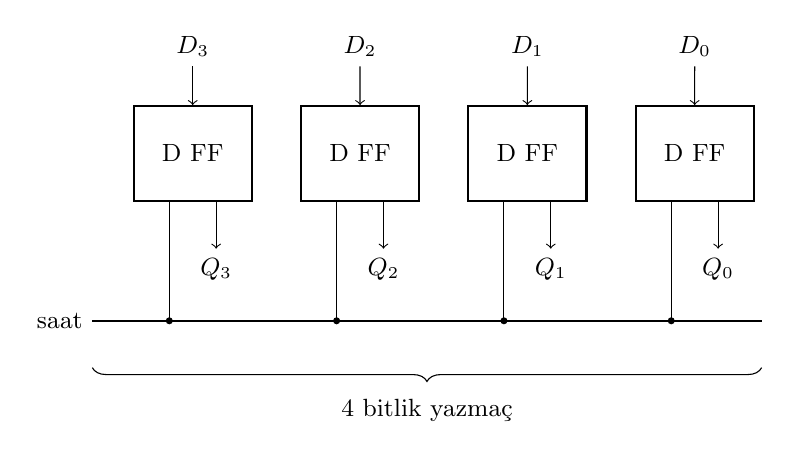
\begin{tikzpicture}[scale=0.85, every node/.style={font=\small},
    dff/.style={draw, thick, minimum width=1.5cm, minimum height=1.2cm}]
  % LSB sağda: bit 3 solda, bit 0 sağda
  \foreach \i [evaluate=\i as \idx using int(3-\i)] in {0,1,2,3} {
    \node[dff] (d\i) at (2.5*\i, 0) {D FF};
    % D girişi üstten ok
    \draw[->] (2.5*\i, 1.3) node[above] {$D_{\idx}$} -- (d\i.north);
    % Q çıkışı: alt-sağ kenardan aşağı ok ile etikete
    \coordinate (q\i) at ([xshift=0.35cm]d\i.south);
    \draw[->] (q\i) -- ++(0, -0.7) node[below] {$Q_{\idx}$};
    % Saat girişi: alt-sol kenardan ortak saat hattına
    \coordinate (clk\i) at ([xshift=-0.35cm]d\i.south);
    \draw (clk\i) -- (clk\i |- 0, -2.5);
    \fill (clk\i |- 0, -2.5) circle (1.5pt);
  }
  % Ortak saat hattı
  \draw[thick] (-1.5, -2.5) -- (8.5, -2.5);
  \node[left] at (-1.5, -2.5) {saat};
  % Brace
  \draw[decorate, decoration={brace, amplitude=5pt, mirror}]
       (-1.5, -3.2) -- (8.5, -3.2)
       node[midway, below=8pt] {4 bitlik yazmaç};
\end{tikzpicture}
\caption{4 bitlik koşut yüklemeli yazmaç}
\label{fig:kosut-yazmac}
\end{figure}

Uygulamada yazmaçlara genellikle bir ``yükleme etkinleştirme'' (İngilizcesi: \textit{load enable}) denetim sinyali eklenir. Bu sinyal etkin düşük ya da etkin yüksek olarak tasarlanabilir; sinyal etkin değilken yazmaç, saat vuruşlarına karşın mevcut değerini korur, etkin olduğunda ise yeni veri yüklenir. Bu sayede yazmaç yalnızca istenildiğinde güncellenir.

\subsection{Kaydırmalı Yazmaç}
\index{kaydırmalı yazmaç}

Kaydırmalı yazmaç (İngilizcesi: \textit{shift register}), her saat vuruşunda saklanan bit dizisini bir konum sağa ya da sola kaydıran bir yazmaçtır. Her D flip-flopunun çıkışı ($Q$), bir sonraki (sağa kaydırmada) ya da bir önceki (sola kaydırmada) flip-flopun girişine ($D$) bağlanır.

Kaydırmalı yazmaçlar çarpma (sola kaydırma $= \times 2$) ve bölme (sağa kaydırma $= \div 2$) işlemlerinde, seri-koşut veri dönüştürmede ve iletişim arabirimlerinde yaygın biçimde kullanılır.

\begin{figure}[H]
\centering
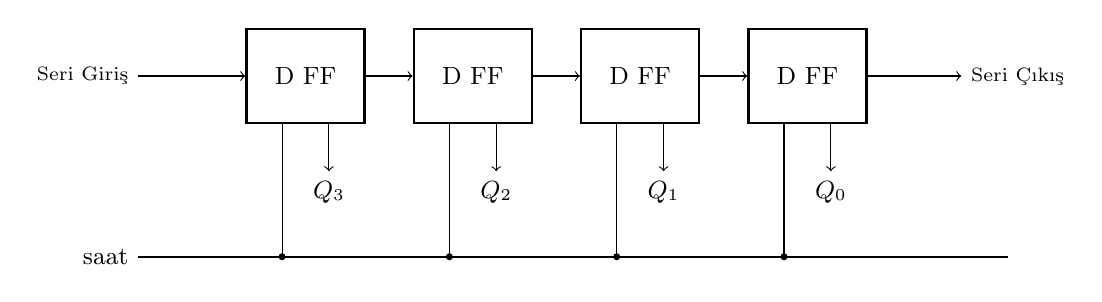
\begin{tikzpicture}[scale=0.85, every node/.style={font=\small},
    dff/.style={draw, thick, minimum width=1.5cm, minimum height=1.2cm}]
  % MSB solda, LSB sağda; sağa kaydırma: veri SG'den (sol) girer, SÇ'den (sağ) çıkar
  \foreach \i [evaluate=\i as \idx using int(3-\i)] in {0,1,2,3} {
    \node[dff] (d\i) at (2.5*\i, 0) {D FF};
    % Saat girişi alt-sol kenardan
    \coordinate (clk\i) at ([xshift=-0.35cm]d\i.south);
    \draw (clk\i) -- (clk\i |- 0, -2.7);
    \fill (clk\i |- 0, -2.7) circle (1.5pt);
    % Q etiketi alt-sağ kenardan
    \coordinate (q\i) at ([xshift=0.35cm]d\i.south);
    \draw[->] (q\i) -- ++(0, -0.7) node[below] {$Q_{\idx}$};
  }
  % Seri giriş (sol kenardan FF1'in D girişine)
  \draw[->] (-2.5, 0) node[left, font=\scriptsize] {Seri Giriş} -- (d0.west);
  % FF zinciri: her Q çıkışı bir sonraki D girişine
  \foreach \i [evaluate=\i as \next using int(\i+1)] in {0,1,2} {
    \draw[->] (d\i.east) -- (d\next.west);
  }
  % Seri çıkış (en sağdaki FF'nin Q'sundan)
  \draw[->] (d3.east) -- ++(1.4, 0) node[right, font=\scriptsize] {Seri Çıkış};
  % Ortak saat hattı
  \draw[thick] (-2.5, -2.7) -- (10.5, -2.7);
  \node[left] at (-2.5, -2.7) {saat};
\end{tikzpicture}
\caption{4 bitlik sağa kaydırmalı yazmaç: seri giriş en soldaki D FF'nin girişine bağlanır; her saat vuruşunda her bit bir konum sağa kayar ve seri çıkıştan çıkar. $Q_3$--$Q_0$ koşut çıkışlardır.}
\label{fig:kaydirmali-yazmac}
\end{figure}

\begin{ornek}[B.14]
4 bitlik bir kaydırmalı yazmaçta başlangıç değeri $1011$ olsun. Sağa üç kez kaydırma yapıldığında ve boşalan en soldaki bite 0 yazıldığında sırayla hangi değerler elde edilir?

\textbf{Çözüm:}
Başlangıç değeri yazmaç girişine yüklenir; ardından her saat vuruşunda tüm bitler bir konum sağa kaydırılır ve soldaki boşalan bite 0 atanır.

\begin{table}[H]
\centering
\begin{tabular}{cl}
\toprule
\textbf{Saat vuruşu} & \textbf{Yazmaç içeriği} \\
\midrule
Başlangıç & $1011$ \\
1.~vuruş   & $0101$ \\
2.~vuruş   & $0010$ \\
3.~vuruş   & $0001$ \\
\bottomrule
\end{tabular}
\end{table}

Başlangıç değeri $1011_2 = 11_{10}$ idi. Her sağa kaydırma ikiye bölmeye karşılık gelir: $11 \to 5 \to 2 \to 1$ (kesirli kısımlar atılır).
\end{ornek}


% =====================================================
\section{Sayaçlar}
\label{sec:sayaclar}
\index{sayaç}

Sayaç (İngilizcesi: \textit{counter}), her saat vuruşunda değerini belirli bir düzende artıran ya da azaltan ardışıl devredir. Bir sayaç, temelde bir yazmaç ile bu yazmacın değerini güncelleyen birleşik mantığın birleşimidir. Sayaçlar, işlemcilerde program sayacı (İngilizcesi: \textit{program counter}) olarak, zamanlama devrelerinde, bellek adresleme birimlerinde ve olay sayma işlemlerinde kullanılır. RISC-V'teki program sayacı, her saat çevriminde 4 artırılan (dallanma durumunda ise hedef adres yüklenen) tipik bir sayaç uygulamasıdır.

\subsection{Eşzamanlı İkili Sayaç}
\index{eşzamanlı sayaç}

Eşzamanlı (İngilizcesi: \textit{synchronous}) sayaçta tüm flip-floplar aynı saat sinyaliyle tetiklenir. $n$ bitlik bir yukarı sayaç, $0$'dan $2^n - 1$'e kadar sayar ve sonra sıfıra döner. Sayacı gerçekleştirmek için T flip-flopları kullanılır: en düşük bit ($T_0$) her zaman terslenirken, $i$.~bit ancak kendisinden düşük tüm bitler $1$ olduğunda terslenmelidir.

\[
T_0 = 1, \qquad T_1 = Q_0, \qquad T_2 = Q_0 \cdot Q_1, \qquad T_i = \prod_{j=0}^{i-1} Q_j
\]

\begin{ornek}[B.15]
3 bitlik eşzamanlı yukarı sayacın sayma dizisi aşağıda çıkarılır.

\textbf{Çözüm:}

\begin{table}[H]
\centering
\begin{tabular}{c|ccc}
\toprule
\textbf{Saat} & $Q_2$ & $Q_1$ & $Q_0$ \\
\midrule
0 & 0 & 0 & 0 \\
1 & 0 & 0 & 1 \\
2 & 0 & 1 & 0 \\
3 & 0 & 1 & 1 \\
4 & 1 & 0 & 0 \\
5 & 1 & 0 & 1 \\
6 & 1 & 1 & 0 \\
7 & 1 & 1 & 1 \\
(8 & 0 & 0 & 0) \\
\bottomrule
\end{tabular}
\end{table}

Sayaç $0$'dan $7$'ye kadar sayar ve saat vuruşu 8'de sıfıra döner. $T_0 = 1$ olduğu için en düşük bit her vuruşta değişir. $T_1 = Q_0$ olduğu için $Q_1$, yalnızca $Q_0 = 1$ olduğu vuruşlarda değişir. $T_2 = Q_0 \cdot Q_1$ olduğu için $Q_2$, ancak her iki alt bit de $1$ olduğunda değişir.
\end{ornek}

\subsection{Eşzamansız (Dalgalı) Sayaç}
\index{eşzamansız sayaç}

Eşzamansız (İngilizcesi: \textit{asynchronous} veya \textit{ripple}) sayaçta yalnızca ilk flip-flop doğrudan saat sinyaliyle tetiklenir; sonraki her flip-flopun saat girişi, bir önceki flip-flopun çıkışına bağlanır. Bu yapı daha basittir, ancak terslenme sinyali basamaktan basamağa gecikmeyle ilerler, elde sinyalinin ``dalga'' gibi yayıldığı bu davranış nedeniyle devre yüksek hızda çalışamaz. Yüksek hız gerektiren uygulamalarda eşzamanlı sayaçlar seçilir.

\begin{figure}[H]
\centering
\begin{tikzpicture}[scale=1, every node/.style={font=\small}]

  % ---- FF0 ----
  \node[flipflop, minimum width=2.2cm, minimum height=2.8cm] (ff0) at (0,0) {};
  \node[font=\footnotesize\bfseries] at (0, 0.85) {T FF};
  % T=1 girisi
  \draw[thick] (ff0.west |- 0,0.45) -- ++(-1.0,0) node[left] {\footnotesize $T{=}1$};
  \node[ffgiris, right] at ([xshift=2pt]ff0.west |- 0,0.45) {$T$};
  % Saat girisi (CLK)
  \draw[thick] (ff0.west |- 0,-0.45) -- ++(-1.0,0) node[left] {\footnotesize Saat};
  \draw ([xshift=2pt]ff0.west |- 0,-0.60) -- ++(0.22,0.15) -- ++(-0.22,0.15);
  % Q cikisi (kisa, T=1 etiketinden uzak)
  \draw (ff0.east |- 0,0.45) -- ++(0.4,0) coordinate (q0wire);
  \node[ffcikis, left] at ([xshift=-2pt]ff0.east |- 0,0.45) {$Q$};
  \node[below=0.5cm] at (ff0.south) {$Q_0$};

  % ---- FF1 ----
  \node[flipflop, minimum width=2.2cm, minimum height=2.8cm] (ff1) at (4.5,0) {};
  \node[font=\footnotesize\bfseries] at (4.5, 0.85) {T FF};
  % T=1 girisi
  \draw[thick] (ff1.west |- 0,0.45) -- ++(-1.0,0) node[left] {\footnotesize $T{=}1$};
  \node[ffgiris, right] at ([xshift=2pt]ff1.west |- 0,0.45) {$T$};
  % Saat girisi (Q0'dan)
  \draw[thick] (ff1.west |- 0,-0.45) -- ++(-1.0,0);
  \draw ([xshift=2pt]ff1.west |- 0,-0.60) -- ++(0.22,0.15) -- ++(-0.22,0.15);
  % Q0 -> CLK1 baglantisi (dikey-yatay, ok başı CLK1'de)
  \draw[okstil] (q0wire) |- (ff1.west |- 0,-0.45);
  % Q cikisi (kisa, T=1 etiketinden uzak)
  \draw (ff1.east |- 0,0.45) -- ++(0.4,0) coordinate (q1wire);
  \node[ffcikis, left] at ([xshift=-2pt]ff1.east |- 0,0.45) {$Q$};
  \node[below=0.5cm] at (ff1.south) {$Q_1$};

  % ---- FF2 ----
  \node[flipflop, minimum width=2.2cm, minimum height=2.8cm] (ff2) at (9.0,0) {};
  \node[font=\footnotesize\bfseries] at (9.0, 0.85) {T FF};
  % T=1 girisi
  \draw[thick] (ff2.west |- 0,0.45) -- ++(-1.0,0) node[left] {\footnotesize $T{=}1$};
  \node[ffgiris, right] at ([xshift=2pt]ff2.west |- 0,0.45) {$T$};
  % Saat girisi (Q1'den)
  \draw[thick] (ff2.west |- 0,-0.45) -- ++(-1.0,0);
  \draw ([xshift=2pt]ff2.west |- 0,-0.60) -- ++(0.22,0.15) -- ++(-0.22,0.15);
  % Q1 -> CLK2 baglantisi (dikey-yatay)
  \draw[okstil] (q1wire) |- (ff2.west |- 0,-0.45);
  % Q cikisi
  \draw[okstil] (ff2.east |- 0,0.45) -- ++(1.2,0) node[right] {\footnotesize $Q_2$};
  \node[ffcikis, left] at ([xshift=-2pt]ff2.east |- 0,0.45) {$Q$};
  \node[below=0.5cm] at (ff2.south) {$Q_2$};

\end{tikzpicture}
\caption{3 bitlik eşzamansız (dalgalı) sayaç: her flip-flopun saat girişi bir önceki flip-flopun çıkışına bağlıdır}
\label{fig:B.eszsiz-sayac}
\end{figure}

\begin{figure}[H]
\centering
\begin{tikzpicture}[yscale=0.7, xscale=1.1]
    \def\cyclew{1.2}   % bir saat çevriminin genişliği
    \def\ncycles{8}    % toplam çevrim sayısı
    \def\sigH{0.8}     % sinyal yüksekliği

    % --- Saat sinyali (CLK) ---
    % Kare dalga: her çevrimde düşen kenar Q0'ı tetikler
    \node[zamanetiket, left] at (-0.3, 0) {Saat};
    \foreach \i in {0,...,7} {
        \pgfmathsetmacro{\xl}{\i*\cyclew}
        \pgfmathsetmacro{\xm}{\i*\cyclew + \cyclew/2}
        \pgfmathsetmacro{\xr}{(\i+1)*\cyclew}
        \draw[zamansinyal] (\xl, 0) -- (\xl, \sigH) -- (\xm, \sigH) -- (\xm, 0) -- (\xr, 0);
    }

    % --- Q0: saat düşen kenarında (xm noktasında) toggle ---
    % Değerler çevrim başında: 0,1,0,1,0,1,0,1 (sonraki: 0)
    % q0vals[i] = i. çevrim süresince Q0'ın değeri
    \node[zamanetiket, left] at (-0.3, -2) {$Q_0$};
    % Çevrim 0: Q0=0, Çevrim 1: Q0=1, ..., düşen kenarda toggle
    % Başlangıç Q0=0, her xm'de (saat düşen kenar) toggle
    \draw[sinyalyesil, very thick] (0, {0*\sigH - 2}) -- ({0.5*\cyclew}, {0*\sigH - 2});
    \draw[sinyalyesil, very thick] ({0.5*\cyclew}, {0*\sigH - 2}) -- ({0.5*\cyclew}, {1*\sigH - 2});
    \draw[sinyalyesil, very thick] ({0.5*\cyclew}, {1*\sigH - 2}) -- ({1.5*\cyclew}, {1*\sigH - 2});
    \draw[sinyalyesil, very thick] ({1.5*\cyclew}, {1*\sigH - 2}) -- ({1.5*\cyclew}, {0*\sigH - 2});
    \draw[sinyalyesil, very thick] ({1.5*\cyclew}, {0*\sigH - 2}) -- ({2.5*\cyclew}, {0*\sigH - 2});
    \draw[sinyalyesil, very thick] ({2.5*\cyclew}, {0*\sigH - 2}) -- ({2.5*\cyclew}, {1*\sigH - 2});
    \draw[sinyalyesil, very thick] ({2.5*\cyclew}, {1*\sigH - 2}) -- ({3.5*\cyclew}, {1*\sigH - 2});
    \draw[sinyalyesil, very thick] ({3.5*\cyclew}, {1*\sigH - 2}) -- ({3.5*\cyclew}, {0*\sigH - 2});
    \draw[sinyalyesil, very thick] ({3.5*\cyclew}, {0*\sigH - 2}) -- ({4.5*\cyclew}, {0*\sigH - 2});
    \draw[sinyalyesil, very thick] ({4.5*\cyclew}, {0*\sigH - 2}) -- ({4.5*\cyclew}, {1*\sigH - 2});
    \draw[sinyalyesil, very thick] ({4.5*\cyclew}, {1*\sigH - 2}) -- ({5.5*\cyclew}, {1*\sigH - 2});
    \draw[sinyalyesil, very thick] ({5.5*\cyclew}, {1*\sigH - 2}) -- ({5.5*\cyclew}, {0*\sigH - 2});
    \draw[sinyalyesil, very thick] ({5.5*\cyclew}, {0*\sigH - 2}) -- ({6.5*\cyclew}, {0*\sigH - 2});
    \draw[sinyalyesil, very thick] ({6.5*\cyclew}, {0*\sigH - 2}) -- ({6.5*\cyclew}, {1*\sigH - 2});
    \draw[sinyalyesil, very thick] ({6.5*\cyclew}, {1*\sigH - 2}) -- ({7.5*\cyclew}, {1*\sigH - 2});
    \draw[sinyalyesil, very thick] ({7.5*\cyclew}, {1*\sigH - 2}) -- ({7.5*\cyclew}, {0*\sigH - 2});
    \draw[sinyalyesil, very thick] ({7.5*\cyclew}, {0*\sigH - 2}) -- ({8*\cyclew},   {0*\sigH - 2});

    % --- Q1: Q0'ın düşen kenarında (xm'de Q0 1->0) toggle ---
    % Q0 1->0 geçişleri: xm=1.5, 3.5, 5.5, 7.5 (çevrim 1,3,5,7'nin ortası)
    % Q1 değerleri: 0(0-1.5), 0->1(1.5), 1(1.5-3.5), 1->0(3.5), 0(3.5-5.5), 0->1(5.5), 1(5.5-7.5), 1->0(7.5), 0
    \node[zamanetiket, left] at (-0.3, -4.5) {$Q_1$};
    \draw[sinyalkirmizi, very thick] (0,             {0*\sigH - 4.5}) -- ({1.5*\cyclew}, {0*\sigH - 4.5});
    \draw[sinyalkirmizi, very thick] ({1.5*\cyclew}, {0*\sigH - 4.5}) -- ({1.5*\cyclew}, {1*\sigH - 4.5});
    \draw[sinyalkirmizi, very thick] ({1.5*\cyclew}, {1*\sigH - 4.5}) -- ({3.5*\cyclew}, {1*\sigH - 4.5});
    \draw[sinyalkirmizi, very thick] ({3.5*\cyclew}, {1*\sigH - 4.5}) -- ({3.5*\cyclew}, {0*\sigH - 4.5});
    \draw[sinyalkirmizi, very thick] ({3.5*\cyclew}, {0*\sigH - 4.5}) -- ({5.5*\cyclew}, {0*\sigH - 4.5});
    \draw[sinyalkirmizi, very thick] ({5.5*\cyclew}, {0*\sigH - 4.5}) -- ({5.5*\cyclew}, {1*\sigH - 4.5});
    \draw[sinyalkirmizi, very thick] ({5.5*\cyclew}, {1*\sigH - 4.5}) -- ({7.5*\cyclew}, {1*\sigH - 4.5});
    \draw[sinyalkirmizi, very thick] ({7.5*\cyclew}, {1*\sigH - 4.5}) -- ({7.5*\cyclew}, {0*\sigH - 4.5});
    \draw[sinyalkirmizi, very thick] ({7.5*\cyclew}, {0*\sigH - 4.5}) -- ({8*\cyclew},   {0*\sigH - 4.5});

    % --- Q2: Q1'in düşen kenarında toggle ---
    % Q1 1->0 geçişleri: 3.5 ve 7.5 (çevrim 3 ve 7'nin ortası)
    % Q2 değerleri: 0(0-3.5), 0->1(3.5), 1(3.5-7.5), 1->0(7.5), 0
    \node[zamanetiket, left] at (-0.3, -7) {$Q_2$};
    \draw[thick, blue!70!black] (0,             {0*\sigH - 7}) -- ({3.5*\cyclew}, {0*\sigH - 7});
    \draw[thick, blue!70!black] ({3.5*\cyclew}, {0*\sigH - 7}) -- ({3.5*\cyclew}, {1*\sigH - 7});
    \draw[thick, blue!70!black] ({3.5*\cyclew}, {1*\sigH - 7}) -- ({7.5*\cyclew}, {1*\sigH - 7});
    \draw[thick, blue!70!black] ({7.5*\cyclew}, {1*\sigH - 7}) -- ({7.5*\cyclew}, {0*\sigH - 7});
    \draw[thick, blue!70!black] ({7.5*\cyclew}, {0*\sigH - 7}) -- ({8*\cyclew},   {0*\sigH - 7});

    % --- Düşen kenar kesikli çizgileri ---
    % Saat düşen kenarları (xm = 0.5, 1.5, ..., 7.5)
    \foreach \i in {0,...,7} {
        \pgfmathsetmacro{\xm}{\i*\cyclew + 0.5*\cyclew}
        \draw[thin, gray, dashed] (\xm, \sigH+0.3) -- (\xm, -7.8);
    }

    % --- Onluk sayım değerleri ---
    % Her çevrimde (çevrim başında) onluk değer: 0,1,2,3,4,5,6,7
    \node[zamanetiket, left] at (-0.3, -8.8) {Onluk};
    \foreach \i/\val in {0/0, 1/1, 2/2, 3/3, 4/4, 5/5, 6/6, 7/7} {
        \pgfmathsetmacro{\xc}{\i*\cyclew + 0.5*\cyclew}
        \node[font=\small] at (\xc, -8.8) {$\val$};
    }
    % Son döngü başı: 0
    \node[font=\small] at ({8*\cyclew}, -8.8) {$0$};

\end{tikzpicture}
\caption[3-bit eşzamansız sayacın dalga formu]{Şekil~\ref{fig:B.eszsiz-sayac}'deki sayacın dalga formu: $Q_0$ her saat düşen kenarında, $Q_1$ ve $Q_2$ ise bir önceki bitin düşen kenarında terslenir. Onluk sayım 0'dan 7'ye yükselir, sonra başa döner.}
\label{fig:B.eszsiz-zamanlama}
\end{figure}

Her flip-flopun tetiklenmesi bir önceki aşamanın çıkışına bağlı olduğundan, yayılma gecikmesi zincir boyunca birikerek artar; yüksek hız gerektiren uygulamalarda bu nedenle eşzamanlı sayaçlar kullanılır.


% =====================================================
\section{Mealy ve Moore Makineleri}
\index{Mealy makinesi}
\index{Moore makinesi}
\index{durum makinesi}

Flip-floplar ve yazmaçlar veri saklar; ancak bir işlemcinin denetim birimi gibi karmaşık bir birim, yalnızca veri saklamakla kalmaz, aynı zamanda ``şu an hangi aşamadayım?'' sorusunu da yanıtlamak zorundadır. Örneğin çok çevrimli bir işlemcide denetim birimi sırayla ``buyruk getir'', ``çöz'', ``yürüt'' gibi aşamalardan geçer. Bu tür davranışlar \textbf{sonlu durum makineleri}\index{sonlu durum makinesi} (İngilizcesi: \emph{finite state machine}, FSM) ile modellenir.

Sonlu durum makineleri, çıkışların nasıl belirlendiğine göre iki temel modele ayrılır: \textbf{Moore} ve \textbf{Mealy} makineleri. Bu iki model, aynı davranışı farklı şekillerde gerçekleştirebilir; hangisinin seçileceği uygulamanın gereksinimlerine bağlıdır.

\begin{tanim}[Mealy Makinesi]
\textbf{Mealy makinesi}\index{Mealy makinesi}, çıkışların hem \emph{mevcut duruma} hem de \emph{mevcut girişlere} bağlı olduğu bir sonlu durum makinesidir. Çıkışlar, girişler değiştiğinde (saat vuruşunu beklemeden) hemen güncellenebilir. Mealy makinesi, George H. Mealy tarafından 1955 yılında tanımlanmıştır~\cite{mealy1955}.
\end{tanim}

\begin{tanim}[Moore Makinesi]
\textbf{Moore makinesi}\index{Moore makinesi}, çıkışların \emph{yalnızca mevcut duruma} bağlı olduğu bir sonlu durum makinesidir. Çıkışlar, durum geçişi tamamlandıktan sonra güncellenir ve bir sonraki saat vuruşuna kadar sabit kalır. Moore makinesi, Edward F. Moore tarafından 1956 yılında tanımlanmıştır~\cite{moore1956}.
\end{tanim}

\subsection{İki Model Arasındaki Farklar}

Mealy ve Moore makinelerinin temel farkları Tablo~\ref{tab:B.moore-mealy}'de özetlenmiştir.

\begin{table}[H]
\centering
\caption{Mealy ve Moore makinelerinin karşılaştırması}
\label{tab:B.moore-mealy}
\begin{tabular}{lcc}
\toprule
\textbf{Özellik} & \textbf{Moore} & \textbf{Mealy} \\
\midrule
Çıkış bağımlılığı & Yalnızca durum & Durum + giriş \\
Çıkış güncellemesi & Saat vuruşunda & Giriş değiştiğinde \\
Durum sayısı & Genellikle daha fazla & Genellikle daha az \\
Çıkış kararlılığı & Daha kararlı & Titreşime açık \\
Tepki hızı & Bir çevrim gecikmeli & Anında tepki \\
Durum diyagramında çıkış & Durumun içinde & Geçiş okları üzerinde \\
\bottomrule
\end{tabular}
\end{table}

\begin{figure}[H]
\centering
\begin{tikzpicture}[yscale=0.72, xscale=1.25]
    \def\cyclew{1.4}   % bir saat çevriminin genişliği
    \def\ncycles{5}    % toplam çevrim sayısı
    \def\sigH{0.75}   % sinyal yüksekliği

    % -------------------------------------------------------
    % YARDIMCI BÜYÜKLÜKLER
    % X 0->1 geçişi: çevrim 1'in ortasından biraz sonra (t=1.5*cyclew)
    % X 1->0 geçişi: çevrim 3'ün ortasından biraz sonra (t=3.5*cyclew)
    % Mealy çıkışı: X ile AYNI anda değişir
    % Moore çıkışı: X'in değiştiği çevrimin BİTİŞİNDE (yükselen kenarda) değişir
    %   0->1 için: çevrim 2 yükselen kenarı = 2*cyclew
    %   1->0 için: çevrim 4 yükselen kenarı = 4*cyclew
    % -------------------------------------------------------

    \pgfmathsetmacro{\txrise}{1.5*\cyclew}    % X yükselme anı
    \pgfmathsetmacro{\txfall}{3.5*\cyclew}    % X düşme anı
    \pgfmathsetmacro{\tmrise}{1.5*\cyclew}    % Mealy yükselme anı (=X)
    \pgfmathsetmacro{\tmfall}{3.5*\cyclew}    % Mealy düşme anı  (=X)
    \pgfmathsetmacro{\torise}{2.0*\cyclew}    % Moore yükselme kenarı
    \pgfmathsetmacro{\tofall}{4.0*\cyclew}    % Moore düşme kenarı
    \pgfmathsetmacro{\tend}{\ncycles*\cyclew} % toplam süre

    % -------------------------------------------------------
    % SAAT SİNYALİ (y=0)
    % -------------------------------------------------------
    \node[zamanetiket, left] at (-0.35, 0) {Saat};
    \foreach \i in {0,...,\the\numexpr\ncycles-1\relax} {
        \pgfmathsetmacro{\xl}{\i*\cyclew}
        \pgfmathsetmacro{\xm}{\i*\cyclew + \cyclew/2}
        \pgfmathsetmacro{\xr}{(\i+1)*\cyclew}
        \draw[zamansinyal] (\xl,0) -- (\xl,\sigH) -- (\xm,\sigH) -- (\xm,0) -- (\xr,0);
    }

    % -------------------------------------------------------
    % YÜKSELEN KENAR KESIKLI ÇIZGILER (tüm sinyalleri keser)
    % -------------------------------------------------------
    \foreach \i in {0,...,\ncycles} {
        \pgfmathsetmacro{\xk}{\i*\cyclew}
        \draw[thin, gray!55, dashed] (\xk, \sigH+0.25) -- (\xk, -8.6);
    }

    % -------------------------------------------------------
    % GİRİŞ X (y=-2.2) — asenkron geçiş, saat kenarına HİZALI DEĞİL
    % -------------------------------------------------------
    \node[zamanetiket, left] at (-0.35, -2.2) {$X$};
    % Başlangıç: 0 (düşük)
    \draw[sinyalkirmizi, very thick] (0, {-2.2}) -- (\txrise, {-2.2});
    % 0->1 geçişi
    \draw[sinyalkirmizi, very thick] (\txrise, {-2.2}) -- (\txrise, {-2.2+\sigH});
    % 1 (yüksek) tutulur
    \draw[sinyalkirmizi, very thick] (\txrise, {-2.2+\sigH}) -- (\txfall, {-2.2+\sigH});
    % 1->0 geçişi
    \draw[sinyalkirmizi, very thick] (\txfall, {-2.2+\sigH}) -- (\txfall, {-2.2});
    % Sona kadar 0
    \draw[sinyalkirmizi, very thick] (\txfall, {-2.2}) -- (\tend, {-2.2});

    % "asenkron" etiketi — X geçişinin altına
    \node[font=\tiny, gray!80] at (\txrise, {-2.2-0.42}) {asenkron};
    \node[font=\tiny, gray!80] at (\txfall, {-2.2-0.42}) {asenkron};

    % -------------------------------------------------------
    % MEALY ÇIKIŞI Y_M (y=-4.7) — X ile aynı anda
    % -------------------------------------------------------
    \node[zamanetiket, left] at (-0.35, -4.7) {$Y_M$};
    \draw[sinyalyesil, very thick] (0, {-4.7}) -- (\tmrise, {-4.7});
    \draw[sinyalyesil, very thick] (\tmrise, {-4.7}) -- (\tmrise, {-4.7+\sigH});
    \draw[sinyalyesil, very thick] (\tmrise, {-4.7+\sigH}) -- (\tmfall, {-4.7+\sigH});
    \draw[sinyalyesil, very thick] (\tmfall, {-4.7+\sigH}) -- (\tmfall, {-4.7});
    \draw[sinyalyesil, very thick] (\tmfall, {-4.7}) -- (\tend, {-4.7});

    % "anında" ok etiketi — Mealy yükselme geçişinin üstüne
    \draw[->, >=Stealth, thick, orange!80!black]
        (\tmrise+0.55, {-4.7+\sigH+0.55})
        node[above, font=\scriptsize\bfseries, orange!80!black] {anında}
        -- (\tmrise+0.05, {-4.7+\sigH+0.08});

    % -------------------------------------------------------
    % MOORE ÇIKIŞI Y_O (y=-7.2) — saat yükselen kenarında
    % -------------------------------------------------------
    \node[zamanetiket, left] at (-0.35, -7.2) {$Y_O$};
    \draw[blue!70!black, very thick] (0, {-7.2}) -- (\torise, {-7.2});
    \draw[blue!70!black, very thick] (\torise, {-7.2}) -- (\torise, {-7.2+\sigH});
    \draw[blue!70!black, very thick] (\torise, {-7.2+\sigH}) -- (\tofall, {-7.2+\sigH});
    \draw[blue!70!black, very thick] (\tofall, {-7.2+\sigH}) -- (\tofall, {-7.2});
    \draw[blue!70!black, very thick] (\tofall, {-7.2}) -- (\tend, {-7.2});

    % "saat kenarı bekler" ok etiketi — Moore yükselme geçişinin üstüne
    \draw[->, >=Stealth, thick, blue!70!black]
        (\torise+0.72, {-7.2+\sigH+0.55})
        node[above, font=\scriptsize\bfseries, blue!70!black, align=center]
            {saat kenarı\\bekler}
        -- (\torise+0.05, {-7.2+\sigH+0.08});

    % -------------------------------------------------------
    % ÇEVRIM ETİKETLERİ (üst)
    % -------------------------------------------------------
    \foreach \i in {1,...,\ncycles} {
        \pgfmathsetmacro{\xmid}{(\i-0.5)*\cyclew}
        \node[font=\tiny, gray] at (\xmid, {\sigH+0.55}) {\i};
    }
    \node[font=\tiny, gray, left] at (-0.05, {\sigH+0.55}) {\#};

\end{tikzpicture}
\caption{Mealy ve Moore makinelerinin zamanlama farkı: Mealy çıkışı $Y_M$ giriş $X$ değiştiği anda hemen güncellenir; Moore çıkışı $Y_O$ ise bir sonraki saat yükselen kenarında değişir. Bu nedenle Mealy daha hızlı tepki verirken Moore titreşime karşı daha kararlıdır.}
\label{fig:B.moore-mealy-zamanlama}
\end{figure}

\subsection{Blok Diyagramları}

İki modelin donanım yapısını karşılaştırmak, aralarındaki farkı anlamak açısından faydalıdır.

\begin{figure}[H]
\centering
\begin{tikzpicture}[
    blok/.style={draw, thick, minimum width=2.8cm, minimum height=1.2cm, align=center, fill=blue!8},
    >=Stealth
]
% Mealy makinesi (üstte, yıl sırası: Mealy 1955 önce)
\node[font=\bfseries] at (2.5,3) {Mealy Makinesi};
\node[blok] (komb1) at (0,2) {Sonraki Durum\\Mantığı};
\node[blok] (reg1) at (4,2) {Durum\\Yazmaçları};
\node[blok] (out1) at (8,2) {Çıkış\\Mantığı};

\draw[->, thick] (-2.2,2) -- node[above, font=\small, pos=0.25] {Giriş} (komb1);
\draw[->, thick] (komb1) -- (reg1);
\draw[->, thick] (reg1) -- (out1);
\draw[->, thick] (out1) -- node[above, font=\small, pos=0.75] {Çıkış} (10.2,2);
\draw[->, thick] (reg1.south) -- ++(0,-0.8) -| (komb1.south);
% Saat: alt-sağ tarafından kutuya (geri besleme okundan ayrı)
\draw[->, thick] (4.6,0.5) node[below, font=\small] {Saat} -- ([xshift=0.6cm]reg1.south);
% Mealy farkı: giriş doğrudan çıkış mantığına (Giriş etiketinden başlar)
\draw[->, thick, red!70!black, dashed] (-2.2,2) -- (-2.2,-0.4) -| (out1.south);
\node[font=\footnotesize, red!70!black, align=center] at (3,-1.1) {Giriş doğrudan çıkış\\mantığını da etkiler};

% Moore makinesi (altta, yıl sırası: Moore 1956 sonra)
\node[font=\bfseries] at (2.5,-2) {Moore Makinesi};
\node[blok] (komb2) at (0,-3) {Sonraki Durum\\Mantığı};
\node[blok] (reg2) at (4,-3) {Durum\\Yazmaçları};
\node[blok] (out2) at (8,-3) {Çıkış\\Mantığı};

\draw[->, thick] (-2.2,-3) -- node[above, font=\small, pos=0.25] {Giriş} (komb2);
\draw[->, thick] (komb2) -- (reg2);
\draw[->, thick] (reg2) -- (out2);
\draw[->, thick] (out2) -- node[above, font=\small, pos=0.75] {Çıkış} (10.2,-3);
\draw[->, thick] (reg2.south) -- ++(0,-0.8) -| (komb2.south);
% Saat: alt-sağ tarafından kutuya (geri besleme okundan ayrı)
\draw[->, thick] (4.6,-4.5) node[below, font=\small] {Saat} -- ([xshift=0.6cm]reg2.south);
\end{tikzpicture}
\caption{Mealy ve Moore makinelerinin blok diyagramları. Saat ortak senkronizasyon sinyalidir; her saat vuruşunda durum yazmaçları yenilenir. Mealy makinesinde giriş sinyali (kesikli kırmızı ok) çıkış mantığını doğrudan etkiler; Moore'da ise çıkışlar yalnızca duruma bağlıdır.}
\label{fig:B.moore-mealy-blok}
\end{figure}

\subsection{Durum Diyagramı Gösterimi}

İki modelin durum diyagramları farklı biçimde çizilir:

\begin{itemize}
    \item \textbf{Moore makinesinde}: Çıkış, durumun \emph{içine} yazılır (durum adı / çıkış). Geçiş okları üzerinde yalnızca giriş koşulu bulunur.
    \item \textbf{Mealy makinesinde}: Çıkış, geçiş \emph{okları üzerine} yazılır (giriş / çıkış biçiminde). Durum düğümlerinde çıkış gösterilmez.
\end{itemize}

Aşağıdaki şekilde aynı davranışı gerçekleştiren bir Moore ve bir Mealy makinesi karşılaştırılmıştır. Sistem, giriş sinyalinde iki ardışık `1' algılandığında çıkışı `1' yapar.

\begin{figure}[H]
\centering
\begin{tikzpicture}[node distance=3cm, >=Stealth]
% Mealy (SOLDA, yıl sırası: 1955 önce)
\node[font=\bfseries] at (2.5, 2.6) {Mealy};
\node[durum, minimum size=1.5cm] (a) at (0,0) {$A$};
\node[durum, minimum size=1.5cm] (b) at (5,0) {$B$};

\draw[durumok] (a) to node[above, font=\small] {1 / 0} (b);
\draw[durumok, bend left=30] (b) to node[below, font=\small] {0 / 0} (a);
\draw[->, >=Stealth, thick, loop above, looseness=8] (a) to node[above, font=\small] {0 / 0} (a);
\draw[->, >=Stealth, thick, loop above, looseness=8] (b) to node[above, font=\small] {1 / 1} (b);
% Mealy kutusu
\draw[rounded corners=8pt, thick, gray!50] (-1, -3.2) rectangle (6, 3.2);

% Moore (SAĞDA, yıl sırası: 1956 sonra)
\node[font=\bfseries] at (10.5, 2.6) {Moore};
\node[durum, minimum size=1.5cm] (s0) at (8,0) {$S_0$ / 0};
\node[durum, minimum size=1.5cm] (s1) at (10.5,0) {$S_1$ / 0};
\node[durum, minimum size=1.5cm] (s2) at (13,0) {$S_2$ / 1};

\draw[durumok] (s0) to node[above, font=\small] {1} (s1);
\draw[durumok] (s1) to node[above, font=\small] {1} (s2);
% S_2 → S_0: derin alt eğri (S_1 → S_0 oku üzerinden)
\draw[durumok, bend left=70] (s2) to node[below, font=\small] {0} (s0);
\draw[durumok, bend left=30] (s1) to node[below, font=\small] {0} (s0);
\draw[->, >=Stealth, thick, loop above, looseness=8] (s0) to node[above, font=\small] {0} (s0);
\draw[->, >=Stealth, thick, loop above, looseness=8] (s2) to node[above, font=\small] {1} (s2);
% Moore kutusu (Mealy ile aynı boy)
\draw[rounded corners=8pt, thick, gray!50] (7, -3.2) rectangle (14, 3.2);
\end{tikzpicture}
\caption{Ardışık iki `1' algılama: Mealy (2 durum, solda) ve Moore (3 durum, sağda) karşılaştırması}
\label{fig:B.moore-mealy-ornek}
\end{figure}

Bu örnekte görüldüğü gibi, Mealy makinesi aynı davranışı daha az durumla gerçekleştirebilmektedir (2 durum yerine 3). Ancak Moore makinesinin çıkışı saat sinyaliyle eşzamanlı olduğundan daha kararlıdır.

\subsection{Kullanım Alanları ve Tercih Kriterleri}

\begin{itemize}
    \item \textbf{Moore makinesi tercih edilir}: Çıkışların kararlı ve titreşimsiz (\emph{glitch-free}) olması gereken durumlarda. Örneğin, denetim birimi tasarımlarında Moore modeli yaygındır çünkü çıkışlar yalnızca saat kenarında değişir.
    \item \textbf{Mealy makinesi tercih edilir}: Hızlı tepki süresi gereken ve daha az donanım kaynağı kullanılması istenen durumlarda. Girişe anında yanıt verebilmesi önemli bir avantajdır.
    \item Uygulamada birçok tasarım, \textbf{kayıtlı çıkışlı Mealy} (\emph{registered-output Mealy}) yaklaşımını kullanır: Mealy makinesinin çıkışları bir yazmaç üzerinden geçirilerek hem hız avantajı korunur hem de çıkış kararlılığı sağlanır.
\end{itemize}

% =====================================================
\subsection{Ardışıl Devre Tasarımı Adımları}
\index{ardışıl devre tasarımı}

Ardışıl devre tasarımı sistematik bir süreçtir; aşağıdaki adımlarla gerçekleştirilir:

\begin{enumerate}
  \item \textbf{Problemin tanımı:} Tasarlanacak devrenin işlevi sözlü olarak tanımlanır; girişler, çıkışlar ve istenen davranış belirlenir.
  \item \textbf{Durumların belirlenmesi:} Davranışı gerçekleştirmek için gereken minimum durum kümesi çıkarılır. Her durum, devrenin ``bellek''inde tutulan farklı bir geçmişi temsil eder.
  \item \textbf{Durum geçiş tablosu:} Her durum--giriş çifti için bir sonraki durum ve çıkış değerleri yazılır. Mealy makinesinde çıkışlar geçişlere, Moore makinesinde durumlara bağlıdır.
  \item \textbf{Durum diyagramı:} Tablo görsel olarak çizilir; durumlar düğüm, geçişler ok olur. Bu adım hataları görsel doğrulamayı kolaylaştırır.
  \item \textbf{Durum kodlaması:} Her duruma ikilik bir kod atanır. $n$ durum için $\lceil \log_2 n \rceil$ flip-flop yeterlidir. Kodlama seçimi sonraki adımdaki sadeleştirmeyi etkiler.
  \item \textbf{Flip-flop seçimi ve uyarma denklemleri:} D, T ya da JK flip-flopu seçilir; her flip-flopun girişi için durum geçiş tablosundan denklem türetilir.
  \item \textbf{Boole sadeleştirme:} Flip-flop ve çıkış denklemleri Karno haritası ya da Boole cebri ile en yalın biçimine indirgenir.
  \item \textbf{Devre çizimi:} Sadeleştirilmiş denklemler kapı düzeyinde çizilerek devre tamamlanır.
\end{enumerate}

Bu adımlar aşağıdaki örnekte bir içecek otomatı makinesi üzerinden gösterilmektedir.

\begin{ornek}[B.16]
\index{otomat makinesi}
\index{ardışıl devre!otomat tasarımı}
\index{Mealy durum makinesi!örnek}
\index{durum makinesi!otomat}
\textbf{Tasarım Örneği: İçecek Otomatı Makinesi.} Bu örnekte basit bir içecek otomatı makinesi tasarlanmaktadır. Makine 1~TL ve 2~TL kabul eder; içecek fiyatı 3~TL'dir. Yeterli para atıldığında içecek verilir ve para üstü varsa iade edilir. Tasarım bir Mealy durum makinesi olarak gerçekleştirilir: içecek verme ve para üstü çıkışları, mevcut durumun yanı sıra atılan paraya (girişe) de bağlıdır; örneğin aynı S2 durumunda 1~TL atılırsa yalnızca içecek verilir, 2~TL atılırsa hem içecek hem para üstü verilir.
\index{durum!tanımı}

\textbf{Adım 1: Durumların belirlenmesi.}

\begin{itemize}[nosep, leftmargin=2em]
    \item \textbf{S0:} Bekleme (toplam $= 0$~TL)
    \item \textbf{S1:} 1~TL alındı
    \item \textbf{S2:} 2~TL alındı
    \item \textbf{S3:} 3+~TL (içecek ver)
\end{itemize}

Girişler: \textbf{BirTL} (1~TL atıldı), \textbf{İkiTL} (2~TL atıldı).
Çıkışlar: \textbf{İçecekVer}, \textbf{ParaÜstü}.

\textbf{Adım 2: Durum geçiş tablosu.}
\index{durum geçiş tablosu}

\begin{table}[H]
\centering
\caption*{Otomat makinesi durum geçiş tablosu}
\label{tab:B.otomat-gecis}
\small
\begin{tabular}{c|cc|cc|cc}
\toprule
\multirow{2}{*}{\textbf{Mevcut Durum}} &
\multicolumn{2}{c|}{\textbf{Giriş}} &
\multicolumn{2}{c|}{\textbf{Sonraki Durum}} &
\multicolumn{2}{c}{\textbf{Çıkış}} \\
 & BirTL & İkiTL & & & İçecekVer & ParaÜstü \\
\midrule
S0 & 0 & 0 & S0 & & 0 & 0 \\
S0 & 1 & 0 & S1 & & 0 & 0 \\
S0 & 0 & 1 & S2 & & 0 & 0 \\
S1 & 0 & 0 & S1 & & 0 & 0 \\
S1 & 1 & 0 & S2 & & 0 & 0 \\
S1 & 0 & 1 & S3 & & 1 & 0 \\
S2 & 0 & 0 & S2 & & 0 & 0 \\
S2 & 1 & 0 & S3 & & 1 & 0 \\
S2 & 0 & 1 & S3 & & 1 & 1 \\
S3 & --- & --- & S0 & & 0 & 0 \\
\bottomrule
\end{tabular}
\end{table}

\noindent S3 durumunda içecek verilir ve makine S0'a döner. S2'den İkiTL ile geçişte para üstü (1~TL) iade edilir.

\textbf{Adım 3: Durum diyagramı.}
\index{durum diyagramı}

\begin{figure}[H]
\centering
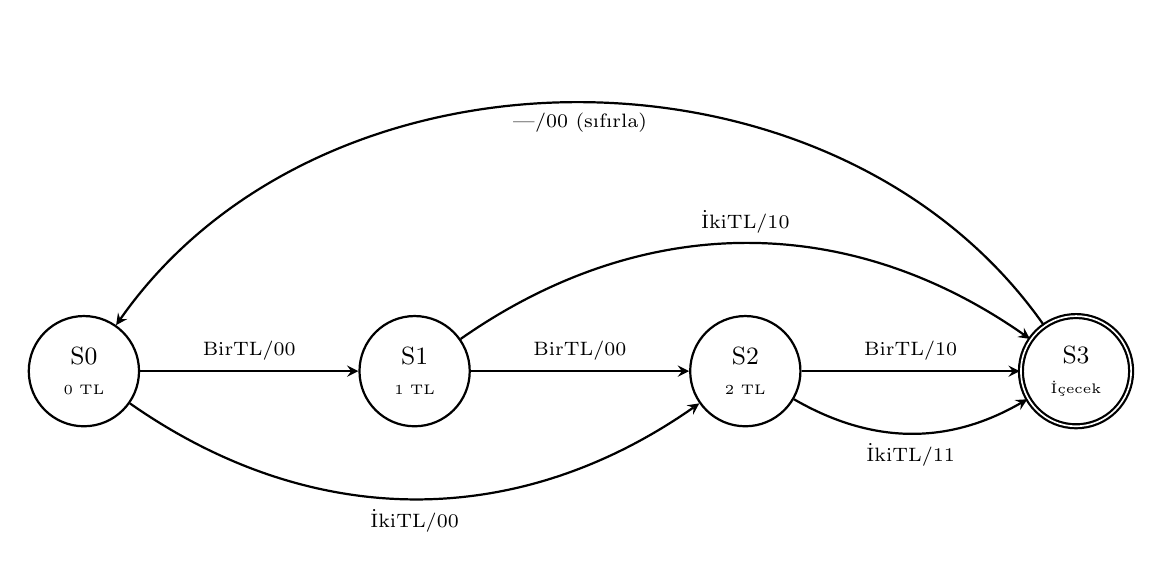
\begin{tikzpicture}[>=stealth, thick, font=\small,
    state/.style={draw, circle, minimum size=1.4cm, inner sep=1pt, align=center}]

% Durumlar (yatay düzen)
\node[state]         (S0) at ( 0,    0) {S0\\{\tiny 0 TL}};
\node[state]         (S1) at ( 4.2,  0) {S1\\{\tiny 1 TL}};
\node[state]         (S2) at ( 8.4,  0) {S2\\{\tiny 2 TL}};
\node[state, double] (S3) at (12.6,  0) {S3\\{\tiny İçecek}};

% Komşu durumlar arası düz geçişler
\draw[->] (S0) -- node[above] {\scriptsize BirTL/00} (S1);
\draw[->] (S1) -- node[above] {\scriptsize BirTL/00} (S2);
\draw[->] (S2) -- node[above] {\scriptsize BirTL/10} (S3);

% Atlamalı geçişler
\draw[->] (S0) to[bend right=35] node[below] {\scriptsize İkiTL/00} (S2);  % alttan
\draw[->] (S1) to[bend left=35]  node[above] {\scriptsize İkiTL/10} (S3);  % üstten

% S2 -> S3 ikinci geçiş (alttan)
\draw[->] (S2) to[bend right=30] node[below] {\scriptsize İkiTL/11} (S3);

% S3 -> S0 (uzun alt kavis: sıfırlama)
\draw[->] (S3) to[bend right=55] node[below] {\scriptsize ---/00 (sıfırla)} (S0);

\end{tikzpicture}
\caption*{Otomat makinesi Mealy durum diyagramı. Geçiş etiketleri ``giriş/çıkış'' biçimindedir; giriş (BirTL,\,İkiTL), çıkış (İçecekVer,\,ParaÜstü). Para girişi olmayan saat tıklarında durum değişmez; bu kendi-üstü geçişler görsel sadelik için çizilmemiştir.}
\label{fig:B.otomat-durum}
\end{figure}

\textbf{Adım 4--5: Durum kodlaması ve flip-flop denklemleri.}
\index{durum kodlaması}
\index{D flip-flop!durum makinesi}

Durumlar 2 bit ile kodlanır: S0$=00$, S1$=01$, S2$=10$, S3$=11$. Mevcut durum bitleri $Q_1 Q_0$, sonraki durum bitleri $D_1 D_0$ olarak adlandırılır.

\begin{table}[H]
\centering
\caption*{Otomat makinesi: kodlanmış durum geçiş tablosu}
\label{tab:B.otomat-kodlu}
\small
\begin{tabular}{cc|cc|cc|cc}
\toprule
\multicolumn{2}{c|}{\textbf{Mevcut}} &
\multicolumn{2}{c|}{\textbf{Giriş}} &
\multicolumn{2}{c|}{\textbf{Sonraki}} &
\multicolumn{2}{c}{\textbf{Çıkış}} \\
$Q_1$ & $Q_0$ & BirTL & İkiTL & $D_1$ & $D_0$ & İçecekVer & ParaÜstü \\
\midrule
0 & 0 & 0 & 0 & 0 & 0 & 0 & 0 \\
0 & 0 & 1 & 0 & 0 & 1 & 0 & 0 \\
0 & 0 & 0 & 1 & 1 & 0 & 0 & 0 \\
0 & 1 & 0 & 0 & 0 & 1 & 0 & 0 \\
0 & 1 & 1 & 0 & 1 & 0 & 0 & 0 \\
0 & 1 & 0 & 1 & 1 & 1 & 1 & 0 \\
1 & 0 & 0 & 0 & 1 & 0 & 0 & 0 \\
1 & 0 & 1 & 0 & 1 & 1 & 1 & 0 \\
1 & 0 & 0 & 1 & 1 & 1 & 1 & 1 \\
1 & 1 & X & X & 0 & 0 & 0 & 0 \\
\bottomrule
\end{tabular}
\end{table}

\textbf{Adım 6--7: Boole sadeleştirme — Karno haritaları.}
\index{Karno haritası!durum makinesi}

Dört değişken ($Q_1, Q_0$, BirTL, İkiTL) üzerinden 2$\times$4 Karno haritaları çizilir. S3 ($Q_1 Q_0 = 11$) durumundan çıkışlar için önemsenmeyen (X) satırı kullanılır.

% --- TikZ makrosu: 4 değişkenli Karno haritası (otomat bölümü) ---
\newcommand{\otomatkarno}[5]{%%
\begin{tikzpicture}[scale=0.6]
    \draw[thick] (0,0) grid (4,4);
    \node[above left, font=\footnotesize] at (0, 4) {$Q_1Q_0$\textbackslash\,BirTL\,İkiTL};
    \node[above, font=\footnotesize] at (0.5, 4) {00};
    \node[above, font=\footnotesize] at (1.5, 4) {01};
    \node[above, font=\footnotesize] at (2.5, 4) {11};
    \node[above, font=\footnotesize] at (3.5, 4) {10};
    \node[left, font=\footnotesize] at (0, 3.5) {00};
    \node[left, font=\footnotesize] at (0, 2.5) {01};
    \node[left, font=\footnotesize] at (0, 1.5) {11};
    \node[left, font=\footnotesize] at (0, 0.5) {10};
    #1 #2 #3 #4 #5
\end{tikzpicture}%%
}

\begin{figure}[H]
\centering
\subcaptionbox{$D_1$\label{fig:B.otomat-D1}}{%%
\otomatkarno%%
  {\node at (0.5,3.5) {0}; \node at (1.5,3.5) {1}; \node[gray] at (2.5,3.5) {X}; \node at (3.5,3.5) {0};}%%
  {\node at (0.5,2.5) {0}; \node at (1.5,2.5) {1}; \node[gray] at (2.5,2.5) {X}; \node at (3.5,2.5) {1};}%%
  {\node[gray] at (0.5,1.5) {X}; \node[gray] at (1.5,1.5) {X}; \node[gray] at (2.5,1.5) {X}; \node[gray] at (3.5,1.5) {X};}%%
  {\node at (0.5,0.5) {1}; \node at (1.5,0.5) {1}; \node[gray] at (2.5,0.5) {X}; \node at (3.5,0.5) {1};}%%
  {% Grup 1: Q1 (satır 10+11, tüm sütunlar — 8 hücre)
   \draw[rounded corners=3pt, ultra thick, sinyalkirmizi, opacity=0.6] (-0.05,0.05) rectangle (3.95,1.95);
   % Grup 2: İkiTL (sütun 01, tüm satırlar — 4 hücre)
   \draw[rounded corners=3pt, ultra thick, sinyalmavi, opacity=0.6] (1.05,0.05) rectangle (1.95,3.95);
   % Grup 3: BirTL·Q0 (satır 01+11, sütun 10 — 2 hücre)
   \draw[rounded corners=3pt, ultra thick, sinyalyesil, opacity=0.6] (3.05,1.05) rectangle (3.95,2.95);
   % Grup sonuç etiketleri (uçlar integer y'de, etiketler dikeyde aralıklı)
   \node[sinyalmavi, anchor=west, font=\footnotesize] (labD1b) at (5, 3.5) {İkiTL};
   \draw[thick, sinyalmavi, opacity=0.7] (1.95, 3) -| (labD1b.west);
   \node[sinyalyesil, anchor=west, font=\footnotesize] (labD1g) at (5, 2) {$Q_0 \cdot$ BirTL};
   \draw[thick, sinyalyesil, opacity=0.7] (3.95, 2) -- (labD1g.west);
   \node[sinyalkirmizi, anchor=west, font=\footnotesize] (labD1r) at (5, 0.5) {$Q_1$};
   \draw[thick, sinyalkirmizi, opacity=0.7] (3.95, 1) -| (labD1r.west);}%%
}\hfill
\subcaptionbox{$D_0$\label{fig:B.otomat-D0}}{%%
\otomatkarno%%
  {\node at (0.5,3.5) {0}; \node at (1.5,3.5) {0}; \node[gray] at (2.5,3.5) {X}; \node at (3.5,3.5) {1};}%%
  {\node at (0.5,2.5) {1}; \node at (1.5,2.5) {1}; \node[gray] at (2.5,2.5) {X}; \node at (3.5,2.5) {0};}%%
  {\node[gray] at (0.5,1.5) {X}; \node[gray] at (1.5,1.5) {X}; \node[gray] at (2.5,1.5) {X}; \node[gray] at (3.5,1.5) {X};}%%
  {\node at (0.5,0.5) {0}; \node at (1.5,0.5) {1}; \node[gray] at (2.5,0.5) {X}; \node at (3.5,0.5) {1};}%%
  {% Grup 1: Q0·B̄irTL (satır 01+11, sütun 00+01 — 4 hücre)
   \draw[rounded corners=3pt, ultra thick, sinyalkirmizi, opacity=0.6] (-0.05,1.05) rectangle (1.95,2.95);
   % Grup 2: Q̄0·BirTL (satır 00+10 kenar sarma, sütun 10 — 2 hücre)
   % Üst yarı: açıklık yukarı bakar (y=4 kenarı), alt yarı: açıklık aşağı bakar (y=0 kenarı)
   \draw[ultra thick, sinyalmavi, opacity=0.6] (3.05,3.95) -- (3.05,3.05) -- (3.95,3.05) -- (3.95,3.95);
   \draw[ultra thick, sinyalmavi, opacity=0.6] (3.05,0.05) -- (3.05,0.95) -- (3.95,0.95) -- (3.95,0.05);
   % Grup 3: Q1·İkiTL (satır 10+11, sütun 01 — 2 hücre)
   \draw[rounded corners=3pt, ultra thick, sinyalyesil, opacity=0.6] (1.05,0.05) rectangle (1.95,1.95);
   % Grup sonuç etiketleri (uçlar integer y'de, etiketler dikeyde aralıklı)
   \node[sinyalmavi, anchor=west, font=\footnotesize] (labD0b) at (5, 3.5) {$\overline{Q_0} \cdot$ BirTL};
   \draw[thick, sinyalmavi, opacity=0.7] (3.95, 3) -| (labD0b.west);
   \node[sinyalkirmizi, anchor=west, font=\footnotesize] (labD0r) at (5, 2) {$Q_0 \cdot \overline{\text{BirTL}}$};
   \draw[thick, sinyalkirmizi, opacity=0.7] (1.95, 2) -- (labD0r.west);
   \node[sinyalyesil, anchor=west, font=\footnotesize] (labD0g) at (5, 0.5) {$Q_1 \cdot$ İkiTL};
   \draw[thick, sinyalyesil, opacity=0.7] (1.95, 1) -| (labD0g.west);}%%
}

\vspace{0.8cm}

\subcaptionbox{İçecekVer\label{fig:B.otomat-IV}}{%%
\otomatkarno%%
  {\node at (0.5,3.5) {0}; \node at (1.5,3.5) {0}; \node[gray] at (2.5,3.5) {X}; \node at (3.5,3.5) {0};}%%
  {\node at (0.5,2.5) {0}; \node at (1.5,2.5) {1}; \node[gray] at (2.5,2.5) {X}; \node at (3.5,2.5) {0};}%%
  {\node[gray] at (0.5,1.5) {X}; \node[gray] at (1.5,1.5) {X}; \node[gray] at (2.5,1.5) {X}; \node[gray] at (3.5,1.5) {X};}%%
  {\node at (0.5,0.5) {0}; \node at (1.5,0.5) {1}; \node[gray] at (2.5,0.5) {X}; \node at (3.5,0.5) {1};}%%
  {% Grup 1: İkiTL·Q0 (satır 01+11, sütun 01 — 2 hücre)
   \draw[rounded corners=3pt, ultra thick, sinyalkirmizi, opacity=0.6] (1.05,1.05) rectangle (1.95,2.95);
   % Grup 2: İkiTL·Q1 (satır 10+11, sütun 01 — 2 hücre)
   \draw[rounded corners=3pt, ultra thick, sinyalmavi, opacity=0.6] (1.05,0.05) rectangle (1.95,1.95);
   % Grup 3: BirTL·Q1 (satır 10+11, sütun 10 — 2 hücre)
   \draw[rounded corners=3pt, ultra thick, sinyalyesil, opacity=0.6] (3.05,0.05) rectangle (3.95,1.95);
   % Grup sonuç etiketleri (uçlar integer y'de, etiketler dikeyde aralıklı)
   \node[sinyalkirmizi, anchor=west, font=\footnotesize] (labIVr) at (5, 3.5) {$Q_0 \cdot$ İkiTL};
   \draw[thick, sinyalkirmizi, opacity=0.7] (1.95, 3) -| (labIVr.west);
   \node[sinyalmavi, anchor=west, font=\footnotesize] (labIVb) at (5, 2) {$Q_1 \cdot$ İkiTL};
   \draw[thick, sinyalmavi, opacity=0.7] (1.95, 1) -| (labIVb.west);
   \node[sinyalyesil, anchor=west, font=\footnotesize] (labIVg) at (5, 0.5) {$Q_1 \cdot$ BirTL};
   \draw[thick, sinyalyesil, opacity=0.7] (3.95, 0) -| (labIVg.west);}%%
}\hfill
\subcaptionbox{ParaÜstü\label{fig:B.otomat-PU}}{%%
\otomatkarno%%
  {\node at (0.5,3.5) {0}; \node at (1.5,3.5) {0}; \node[gray] at (2.5,3.5) {X}; \node at (3.5,3.5) {0};}%%
  {\node at (0.5,2.5) {0}; \node at (1.5,2.5) {0}; \node[gray] at (2.5,2.5) {X}; \node at (3.5,2.5) {0};}%%
  {\node[gray] at (0.5,1.5) {X}; \node[gray] at (1.5,1.5) {X}; \node[gray] at (2.5,1.5) {X}; \node[gray] at (3.5,1.5) {X};}%%
  {\node at (0.5,0.5) {0}; \node at (1.5,0.5) {1}; \node[gray] at (2.5,0.5) {X}; \node at (3.5,0.5) {0};}%%
  {% Grup: İkiTL·Q1 (satır 10+11, sütun 01 — 2 hücre)
   \draw[rounded corners=3pt, ultra thick, sinyalkirmizi, opacity=0.6] (1.05,0.05) rectangle (1.95,1.95);
   % Grup sonuç etiketi (uç integer y'de — grid çizgisinde)
   \node[sinyalkirmizi, anchor=west, font=\footnotesize] (labPUr) at (5, 1) {$Q_1 \cdot$ İkiTL};
   \draw[thick, sinyalkirmizi, opacity=0.7] (1.95, 1) -- (labPUr.west);}%%
}
\caption*{Otomat makinesi: D flip-flop ve çıkış Karno haritaları}
\label{fig:B.otomat-karno}
\end{figure}

Karno haritalarından elde edilen sadeleştirilmiş ifadeler (S3 durumu ile eşzamanlı para atma durumu, BirTL$=$İkiTL$=1$, önemsenmeyen durum olarak ele alınmıştır):

\[
\begin{aligned}
D_1          &= Q_1 + \text{İkiTL} + Q_0 \cdot \text{BirTL} \\
D_0          &= \overline{Q_0} \cdot \text{BirTL}
                 + Q_0 \cdot \overline{\text{BirTL}}
                 + Q_1 \cdot \text{İkiTL} \\
\text{İçecekVer} &= \text{İkiTL} \cdot (Q_0 + Q_1) + \text{BirTL} \cdot Q_1 \\
\text{ParaÜstü}  &= Q_1 \cdot \text{İkiTL}
\end{aligned}
\]

Bu örnekte flip-floplar, durum makinesi kavramı ve birleşik mantık birlikte çalışmaktadır: flip-floplar durumu saklar, birleşik devre ise sonraki durumu ve çıkışları hesaplar.

İşlemci tasarımında kullanılan denetim birimleri de özünde birer durum makinesidir. Bölüm~\ref{chap:islemci-tasarimi}'da göreceğimiz tek vuruşluk ve çok vuruşluk işlemci denetim birimleri, burada öğrendiğimiz ardışıl tasarım ilkelerinin doğrudan uygulamalarıdır.

\end{ornek}

\begin{ornek}[B.17]
\index{durum makinesi!yarışma sistemi}
\index{ardışıl devre!yarışma sistemi}
\index{JK flip-flop!tasarım örneği}
\textbf{Tasarım Örneği: Yarışma Sistemi.} Daha kapsamlı bir örnek olarak iki yarışmacı (A ve B) arasındaki son iki sorunun cevaplarını izleyen bir yarışma sistemi tasarlansın. Sistemin çıkışları aşağıdaki tabloda gösterilmiştir:

\begin{table}[H]
\centering
\caption*{A ve B'nin doğru sayılarına göre çıktı tablosu}
\label{tab:B.16}
\begin{tabular}{l|c}
\toprule
\textbf{Durum} & \textbf{Çıkış} \\
\midrule
Eşit & 000 \\
A, B'den 2 fazla doğru & 001 \\
A, B'den 1 fazla doğru & 010 \\
B, A'dan 1 fazla doğru & 011 \\
B, A'dan 2 fazla doğru & 100 \\
\bottomrule
\end{tabular}
\end{table}

Sistem üç durumda bulunabilir:
\begin{itemize}
    \item Eşit durumu: $xy = 00$
    \item A önde durumu: $xy = 01$
    \item B önde durumu: $xy = 10$
\end{itemize}

\begin{figure}[H]
\centering
\begin{tikzpicture}[node distance=2.8cm]
  % Durumlar
  \node[durum, minimum size=1.4cm, align=center] (esit) {\footnotesize Eşit\\\tiny $xy{=}00$};
  \node[durum, minimum size=1.4cm, align=center, below right of=esit, xshift=0.5cm] (bonde) {\footnotesize B Önde\\\tiny $xy{=}10$};
  \node[durum, minimum size=1.4cm, align=center, below left of=esit, xshift=-0.5cm] (aonde) {\footnotesize A Önde\\\tiny $xy{=}01$};

  % Kendine geçişler
  \draw[->, >=Stealth, thick, loop above, looseness=8] (esit) to node[above, font=\footnotesize] {$AB{=}00,11$} (esit);
  \draw[->, >=Stealth, thick, loop left, looseness=8] (aonde) to node[left, font=\footnotesize] {$AB{=}10,11$} (aonde);
  \draw[->, >=Stealth, thick, loop right, looseness=8] (bonde) to node[right, font=\footnotesize] {$AB{=}01,11$} (bonde);

  % Eşit ↔ A Önde (zıt yönlerdeki büküm fiziksel olarak farklı taraflara düşer)
  \draw[durumok, bend left=20] (esit) to node[above, sloped, font=\footnotesize] {$AB{=}10$} (aonde);
  \draw[durumok, bend left=20] (aonde) to node[above, sloped, font=\footnotesize] {$AB{=}00,01$} (esit);

  % Eşit ↔ B Önde
  \draw[durumok, bend left=20] (esit) to node[above, sloped, font=\footnotesize] {$AB{=}01$} (bonde);
  \draw[durumok, bend left=20] (bonde) to node[above, sloped, font=\footnotesize] {$AB{=}00,10$} (esit);
\end{tikzpicture}
\caption*{Yarışma örneği durum şeması}
\end{figure}

\begin{table}[H]
\centering
\caption*{Yarışma örneği durumlara göre çıkış değerleri}
\label{tab:B.17}
\small
\begin{tabular}{cccc|cc|ccc}
\toprule
$x$ & $y$ & $A$ & $B$ & $x(t+1)$ & $y(t+1)$ & $\text{Ç}_2$ & $\text{Ç}_1$ & $\text{Ç}_0$ \\
\midrule
0 & 0 & 0 & 0 & 0 & 0 & 0 & 0 & 0 \\
0 & 0 & 0 & 1 & 1 & 0 & 0 & 1 & 1 \\
0 & 0 & 1 & 0 & 0 & 1 & 0 & 1 & 0 \\
0 & 0 & 1 & 1 & 0 & 0 & 0 & 0 & 0 \\
0 & 1 & 0 & 0 & 0 & 0 & 0 & 1 & 0 \\
0 & 1 & 0 & 1 & 0 & 0 & 0 & 0 & 0 \\
0 & 1 & 1 & 0 & 0 & 1 & 0 & 0 & 1 \\
0 & 1 & 1 & 1 & 0 & 1 & 0 & 1 & 0 \\
1 & 0 & 0 & 0 & 0 & 0 & 0 & 1 & 1 \\
1 & 0 & 0 & 1 & 1 & 0 & 1 & 0 & 0 \\
1 & 0 & 1 & 0 & 0 & 0 & 0 & 0 & 0 \\
1 & 0 & 1 & 1 & 1 & 0 & 0 & 1 & 1 \\
1 & 1 & X & X & X & X & X & X & X \\
\bottomrule
\end{tabular}
\end{table}

Tasarımda JK flip-flopları kullanılacaktır. JK flip-flopunun geçiş tablosu aşağıda verilmiştir:

\begin{table}[H]
\centering
\caption*{JK flip-flopta $J$ ve $K$ değerleri için doğruluk tablosu}
\label{tab:B.18}
\begin{tabular}{cc|cc|l}
\toprule
$x$ & $x(t+1)$ & $J_x$ & $K_x$ & \textbf{Açıklama} \\
\midrule
0 & 0 & 0 & X & Sıfırla ya da aynı kal \\
0 & 1 & 1 & X & Birle ya da tersle \\
1 & 0 & X & 1 & Sıfırla ya da tersle \\
1 & 1 & X & 0 & Birle ya da aynı kal \\
\bottomrule
\end{tabular}
\end{table}

Bu geçiş tablosu kullanılarak tüm sistemin doğruluk tablosu oluşturulur:

\begin{table}[H]
\centering
\caption*{Tüm sistem için doğruluk tablosu}
\label{tab:B.19}
\small
\begin{tabular}{cccc|cc|ccc|cccc}
\toprule
$x$ & $y$ & $A$ & $B$ & $x(t+1)$ & $y(t+1)$ & $\text{Ç}_2$ & $\text{Ç}_1$ & $\text{Ç}_0$ & $J_x$ & $K_x$ & $J_y$ & $K_y$ \\
\midrule
0 & 0 & 0 & 0 & 0 & 0 & 0 & 0 & 0 & 0 & X & 0 & X \\
0 & 0 & 0 & 1 & 1 & 0 & 0 & 1 & 1 & 1 & X & 0 & X \\
0 & 0 & 1 & 0 & 0 & 1 & 0 & 1 & 0 & 0 & X & 1 & X \\
0 & 0 & 1 & 1 & 0 & 0 & 0 & 0 & 0 & 0 & X & 0 & X \\
0 & 1 & 0 & 0 & 0 & 0 & 0 & 1 & 0 & 0 & X & X & 1 \\
0 & 1 & 0 & 1 & 0 & 0 & 0 & 0 & 0 & 0 & X & X & 1 \\
0 & 1 & 1 & 0 & 0 & 1 & 0 & 0 & 1 & 0 & X & X & 0 \\
0 & 1 & 1 & 1 & 0 & 1 & 0 & 1 & 0 & 0 & X & X & 0 \\
1 & 0 & 0 & 0 & 0 & 0 & 0 & 1 & 1 & X & 1 & 0 & X \\
1 & 0 & 0 & 1 & 1 & 0 & 1 & 0 & 0 & X & 0 & 0 & X \\
1 & 0 & 1 & 0 & 0 & 0 & 0 & 0 & 0 & X & 1 & 0 & X \\
1 & 0 & 1 & 1 & 1 & 0 & 0 & 1 & 1 & X & 0 & 0 & X \\
1 & 1 & 0 & 0 & X & X & X & X & X & X & X & X & X \\
1 & 1 & 0 & 1 & X & X & X & X & X & X & X & X & X \\
1 & 1 & 1 & 0 & X & X & X & X & X & X & X & X & X \\
1 & 1 & 1 & 1 & X & X & X & X & X & X & X & X & X \\
\bottomrule
\end{tabular}
\end{table}

Her bir çıkış fonksiyonu ve flip-flop girişleri Karno haritası ile sadeleştirilir:

% --- TikZ makrosu: Karno haritası (sayaç bölümü, 4 değişken) ---
\newcommand{\sayackarno}[5]{%%
\begin{tikzpicture}[scale=0.6]
    \draw[thick] (0,0) grid (4,4);
    \node[above left, font=\footnotesize] at (0, 4) {$xy$\textbackslash\,$AB$};
    \node[above, font=\footnotesize] at (0.5, 4) {00};
    \node[above, font=\footnotesize] at (1.5, 4) {01};
    \node[above, font=\footnotesize] at (2.5, 4) {11};
    \node[above, font=\footnotesize] at (3.5, 4) {10};
    \node[left, font=\footnotesize] at (0, 3.5) {00};
    \node[left, font=\footnotesize] at (0, 2.5) {01};
    \node[left, font=\footnotesize] at (0, 1.5) {11};
    \node[left, font=\footnotesize] at (0, 0.5) {10};
    #1 #2 #3 #4 #5
\end{tikzpicture}%%
}

\begin{figure}[H]
\centering
% --- Satır 1: Ç2, Ç1 ---
\subcaptionbox{$\text{Ç}_2$}{%%
\sayackarno%%
  {\node at (0.5,3.5) {0}; \node at (1.5,3.5) {0}; \node at (2.5,3.5) {0}; \node at (3.5,3.5) {0};}%%
  {\node at (0.5,2.5) {0}; \node at (1.5,2.5) {0}; \node at (2.5,2.5) {0}; \node at (3.5,2.5) {0};}%%
  {\node[gray] at (0.5,1.5) {X}; \node[gray] at (1.5,1.5) {X}; \node[gray] at (2.5,1.5) {X}; \node[gray] at (3.5,1.5) {X};}%%
  {\node at (0.5,0.5) {0}; \node at (1.5,0.5) {1}; \node at (2.5,0.5) {0}; \node at (3.5,0.5) {0};}%%
  {% Grup: x·Ā·B (sütun 01, satır 10+11 — 2 hücre, X yardımıyla)
   \draw[rounded corners=3pt, ultra thick, sinyalkirmizi, opacity=0.6] (1.05,0.05) rectangle (1.95,1.95);
   \node[sinyalkirmizi, anchor=west, font=\footnotesize] (labC2r) at (5, 1) {$x \cdot \overline{A} \cdot B$};
   \draw[thick, sinyalkirmizi, opacity=0.7] (1.95, 1) -- (labC2r.west);}%%
}\hfill
\subcaptionbox{$\text{Ç}_1$}{%%
\sayackarno%%
  {\node at (0.5,3.5) {0}; \node at (1.5,3.5) {1}; \node at (2.5,3.5) {0}; \node at (3.5,3.5) {1};}%%
  {\node at (0.5,2.5) {1}; \node at (1.5,2.5) {0}; \node at (2.5,2.5) {1}; \node at (3.5,2.5) {0};}%%
  {\node[gray] at (0.5,1.5) {X}; \node[gray] at (1.5,1.5) {X}; \node[gray] at (2.5,1.5) {X}; \node[gray] at (3.5,1.5) {X};}%%
  {\node at (0.5,0.5) {1}; \node at (1.5,0.5) {0}; \node at (2.5,0.5) {1}; \node at (3.5,0.5) {0};}%%
  {% 6 ayrı 2-hücreli/1-hücreli grup, her biri ayrı renk + minterm etiketi
   % Grup 1 kırmızı: x̄ȳĀB — satır 00 sütun 01 (1 hücre, izole)
   \draw[rounded corners=3pt, ultra thick, sinyalkirmizi, opacity=0.6] (1.05,3.05) rectangle (1.95,3.95);
   \node[sinyalkirmizi, anchor=west, font=\footnotesize] (labC1a) at (5, 3.5) {$\overline{x}\,\overline{y}\,\overline{A}\,B$};
   \draw[thick, sinyalkirmizi, opacity=0.7] (1.95, 3) -| (labC1a.west);
   % Grup 2 mavi: x̄ȳAB̄ — satır 00 sütun 10 (1 hücre, izole)
   \draw[rounded corners=3pt, ultra thick, sinyalmavi, opacity=0.6] (3.05,3.05) rectangle (3.95,3.95);
   \node[sinyalmavi, anchor=west, font=\footnotesize] (labC1b) at (5, 2.8) {$\overline{x}\,\overline{y}\,A\,\overline{B}$};
   \draw[thick, sinyalmavi, opacity=0.7] (3.95, 3) -| (labC1b.west);
   % Grup 3 yeşil: yĀB̄ — sütun 00 satır 01+11 (X yardımıyla)
   \draw[rounded corners=3pt, ultra thick, sinyalyesil, opacity=0.6] (-0.05,1.05) rectangle (0.95,2.95);
   \node[sinyalyesil, anchor=east, font=\footnotesize] (labC1c) at (-1.5, 2) {$y\,\overline{A}\,\overline{B}$};
   \draw[thick, sinyalyesil, opacity=0.7] (-0.05, 2) -- (labC1c.east);
   % Grup 4 turuncu: xĀB̄ — sütun 00 satır 10+11 (X yardımıyla)
   \draw[rounded corners=3pt, ultra thick, orange, opacity=0.6] (-0.05,0.05) rectangle (0.95,1.95);
   \node[orange, anchor=east, font=\footnotesize] (labC1d) at (-1.5, 1) {$x\,\overline{A}\,\overline{B}$};
   \draw[thick, orange, opacity=0.7] (-0.05, 1) -- (labC1d.east);
   % Grup 5 mor: yAB — sütun 11 satır 01+11 (X yardımıyla)
   \draw[rounded corners=3pt, ultra thick, purple, opacity=0.6] (2.05,1.05) rectangle (2.95,2.95);
   \node[purple, anchor=west, font=\footnotesize] (labC1e) at (5, 2) {$y\,A\,B$};
   \draw[thick, purple, opacity=0.7] (2.95, 2) -- (labC1e.west);
   % Grup 6 kahverengi: xAB — sütun 11 satır 10+11 (X yardımıyla)
   \draw[rounded corners=3pt, ultra thick, brown, opacity=0.6] (2.05,0.05) rectangle (2.95,1.95);
   \node[brown, anchor=west, font=\footnotesize] (labC1f) at (5, 1.2) {$x\,A\,B$};
   \draw[thick, brown, opacity=0.7] (2.95, 1) -| (labC1f.west);}%%
}

\bigskip
% --- Satır 2: Ç0, Jx ---
\subcaptionbox{$\text{Ç}_0$}{%%
\sayackarno%%
  {\node at (0.5,3.5) {0}; \node at (1.5,3.5) {1}; \node at (2.5,3.5) {0}; \node at (3.5,3.5) {0};}%%
  {\node at (0.5,2.5) {0}; \node at (1.5,2.5) {0}; \node at (2.5,2.5) {0}; \node at (3.5,2.5) {1};}%%
  {\node[gray] at (0.5,1.5) {X}; \node[gray] at (1.5,1.5) {X}; \node[gray] at (2.5,1.5) {X}; \node[gray] at (3.5,1.5) {X};}%%
  {\node at (0.5,0.5) {1}; \node at (1.5,0.5) {0}; \node at (2.5,0.5) {1}; \node at (3.5,0.5) {0};}%%
  {% Grup 1 kırmızı: x̄ȳĀB — satır 00 sütun 01 (1 hücre)
   \draw[rounded corners=3pt, ultra thick, sinyalkirmizi, opacity=0.6] (1.05,3.05) rectangle (1.95,3.95);
   % Grup 2 mavi: x̄yAB̄ — satır 01 sütun 10 (1 hücre)
   \draw[rounded corners=3pt, ultra thick, sinyalmavi, opacity=0.6] (3.05,2.05) rectangle (3.95,2.95);
   % Grup 3 yeşil: x·Ā·B̄ — sütun 00, satır 10+11 (2 hücre, X yardımıyla)
   \draw[rounded corners=3pt, ultra thick, sinyalyesil, opacity=0.6] (-0.05,0.05) rectangle (0.95,1.95);
   % Grup 4 turuncu: x·A·B — sütun 11, satır 10+11 (2 hücre, X yardımıyla)
   \draw[rounded corners=3pt, ultra thick, orange, opacity=0.6] (2.05,0.05) rectangle (2.95,1.95);
   % Etiketler: kırmızı+mavi sağda, yeşil+turuncu aşağıda
   \node[sinyalkirmizi, anchor=west, font=\footnotesize] (labC0r) at (5, 3.5) {$\overline{x}\,\overline{y}\,\overline{A}\,B$};
   \draw[thick, sinyalkirmizi, opacity=0.7] (1.95, 3) -| (labC0r.west);
   \node[sinyalmavi, anchor=west, font=\footnotesize] (labC0b) at (5, 2.5) {$\overline{x}\,y\,A\,\overline{B}$};
   \draw[thick, sinyalmavi, opacity=0.7] (3.95, 2) -| (labC0b.west);
   \node[sinyalyesil, anchor=north, font=\footnotesize] (labC0g) at (0.5, -0.5) {$x\,\overline{A}\,\overline{B}$};
   \draw[thick, sinyalyesil, opacity=0.7] (0.5, 0) -- (0.5, -0.4);
   \node[orange, anchor=north, font=\footnotesize] (labC0o) at (2.5, -0.5) {$x\,A\,B$};
   \draw[thick, orange, opacity=0.7] (2.5, 0) -- (2.5, -0.4);}%%
}\hfill
\subcaptionbox{$J_x$}{%%
\sayackarno%%
  {\node at (0.5,3.5) {0}; \node at (1.5,3.5) {1}; \node at (2.5,3.5) {0}; \node at (3.5,3.5) {0};}%%
  {\node at (0.5,2.5) {0}; \node at (1.5,2.5) {0}; \node at (2.5,2.5) {0}; \node at (3.5,2.5) {0};}%%
  {\node[gray] at (0.5,1.5) {X}; \node[gray] at (1.5,1.5) {X}; \node[gray] at (2.5,1.5) {X}; \node[gray] at (3.5,1.5) {X};}%%
  {\node[gray] at (0.5,0.5) {X}; \node[gray] at (1.5,0.5) {X}; \node[gray] at (2.5,0.5) {X}; \node[gray] at (3.5,0.5) {X};}%%
  {% Grup: ȳ·Ā·B — sütun 01, satır 00+10 sarmalı (2 hücre, X yardımıyla genişler)
   % Üst yarı (satır 00): açık kenarlı üstten
   \draw[ultra thick, sinyalkirmizi, opacity=0.6] (1.05,3.95) -- (1.05,3.05) -- (1.95,3.05) -- (1.95,3.95);
   % Alt yarı (satır 10): açık kenarlı alttan
   \draw[ultra thick, sinyalkirmizi, opacity=0.6] (1.05,0.05) -- (1.05,0.95) -- (1.95,0.95) -- (1.95,0.05);
   \node[sinyalkirmizi, anchor=west, font=\footnotesize] (labJxr) at (5, 2) {$\overline{y} \cdot \overline{A} \cdot B$};
   \draw[thick, sinyalkirmizi, opacity=0.7] (1.95, 3) -| (labJxr.west);}%%
}

\bigskip
% --- Satır 3: Kx, Jy ---
\subcaptionbox{$K_x$}{%%
\sayackarno%%
  {\node[gray] at (0.5,3.5) {X}; \node[gray] at (1.5,3.5) {X}; \node[gray] at (2.5,3.5) {X}; \node[gray] at (3.5,3.5) {X};}%%
  {\node[gray] at (0.5,2.5) {X}; \node[gray] at (1.5,2.5) {X}; \node[gray] at (2.5,2.5) {X}; \node[gray] at (3.5,2.5) {X};}%%
  {\node[gray] at (0.5,1.5) {X}; \node[gray] at (1.5,1.5) {X}; \node[gray] at (2.5,1.5) {X}; \node[gray] at (3.5,1.5) {X};}%%
  {\node at (0.5,0.5) {1}; \node at (1.5,0.5) {0}; \node at (2.5,0.5) {0}; \node at (3.5,0.5) {1};}%%
  {% Grup: B̄ — sütun 00+10 sarmalı (yatay sarma; sol grubun solu, sağ grubun sağı açık)
   % Sol yarı (sütun 00): sol kenar açık
   \draw[ultra thick, sinyalkirmizi, opacity=0.6] (-0.05,3.95) -- (0.95,3.95) -- (0.95,0.05) -- (-0.05,0.05);
   % Sağ yarı (sütun 10): sağ kenar açık
   \draw[ultra thick, sinyalkirmizi, opacity=0.6] (3.95,3.95) -- (3.05,3.95) -- (3.05,0.05) -- (3.95,0.05);
   \node[sinyalkirmizi, anchor=west, font=\footnotesize] (labKxr) at (5, 2) {$\overline{B}$};
   \draw[thick, sinyalkirmizi, opacity=0.7] (3.95, 2) -- (labKxr.west);}%%
}\hfill
\subcaptionbox{$J_y$}{%%
\sayackarno%%
  {\node at (0.5,3.5) {0}; \node at (1.5,3.5) {0}; \node at (2.5,3.5) {0}; \node at (3.5,3.5) {1};}%%
  {\node[gray] at (0.5,2.5) {X}; \node[gray] at (1.5,2.5) {X}; \node[gray] at (2.5,2.5) {X}; \node[gray] at (3.5,2.5) {X};}%%
  {\node[gray] at (0.5,1.5) {X}; \node[gray] at (1.5,1.5) {X}; \node[gray] at (2.5,1.5) {X}; \node[gray] at (3.5,1.5) {X};}%%
  {\node at (0.5,0.5) {0}; \node at (1.5,0.5) {0}; \node at (2.5,0.5) {0}; \node at (3.5,0.5) {0};}%%
  {% Grup: x̄·A·B̄ — sütun 10, satır 00+01 (2 hücre, X yardımıyla)
   \draw[rounded corners=3pt, ultra thick, sinyalkirmizi, opacity=0.6] (3.05,2.05) rectangle (3.95,3.95);
   \node[sinyalkirmizi, anchor=west, font=\footnotesize] (labJyr) at (5, 3) {$\overline{x} \cdot A \cdot \overline{B}$};
   \draw[thick, sinyalkirmizi, opacity=0.7] (3.95, 3) -- (labJyr.west);}%%
}

\bigskip
% --- Satır 4: Ky (tek) ---
\subcaptionbox{$K_y$}{%%
\sayackarno%%
  {\node[gray] at (0.5,3.5) {X}; \node[gray] at (1.5,3.5) {X}; \node[gray] at (2.5,3.5) {X}; \node[gray] at (3.5,3.5) {X};}%%
  {\node at (0.5,2.5) {1}; \node at (1.5,2.5) {1}; \node at (2.5,2.5) {0}; \node at (3.5,2.5) {0};}%%
  {\node[gray] at (0.5,1.5) {X}; \node[gray] at (1.5,1.5) {X}; \node[gray] at (2.5,1.5) {X}; \node[gray] at (3.5,1.5) {X};}%%
  {\node[gray] at (0.5,0.5) {X}; \node[gray] at (1.5,0.5) {X}; \node[gray] at (2.5,0.5) {X}; \node[gray] at (3.5,0.5) {X};}%%
  {% Grup: Ā — sütun 00+01 (tüm satırlar, X yardımıyla)
   \draw[rounded corners=3pt, ultra thick, sinyalkirmizi, opacity=0.6] (-0.05,0.05) rectangle (1.95,3.95);
   \node[sinyalkirmizi, anchor=west, font=\footnotesize] (labKyr) at (5, 2) {$\overline{A}$};
   \draw[thick, sinyalkirmizi, opacity=0.7] (1.95, 2) -- (labKyr.west);}%%
}
\caption*{Sayaç tasarımı Karno haritaları}
\end{figure}

Karno haritalarından elde edilen sadeleştirilmiş ifadeler şunlardır:

\[
\begin{aligned}
J_x &= \overline{y} \cdot \overline{A} \cdot B &\qquad K_x &= \overline{B} \\
J_y &= \overline{x} \cdot A \cdot \overline{B} &\qquad K_y &= \overline{A}
\end{aligned}
\]

Flip-flop giriş ifadeleri oldukça yalındır: $x$ flip-flopu yalnızca B doğru yanıtladığında kurulur ($J_x = \overline{y}\,\overline{A}\,B$) ve B yanlış yanıtladığında sıfırlanır ($K_x = \overline{B}$). Benzer şekilde $y$ flip-flopu yalnızca A doğru yanıtladığında kurulur ($J_y = \overline{x}\,A\,\overline{B}$) ve A yanlış yanıtladığında sıfırlanır ($K_y = \overline{A}$).

\[
\begin{aligned}
\text{Ç}_2 &= x \cdot \overline{A} \cdot B \\
\text{Ç}_1 &= \overline{x}\,\overline{y}\,(A \oplus B) + (x + y) \cdot (A \odot B) \\
\text{Ç}_0 &= \overline{x}\,\overline{y}\,\overline{A}\,B + \overline{x}\,y\,A\,\overline{B} + x\,\overline{A}\,\overline{B} + x\,A\,B
\end{aligned}
\]

$\text{Ç}_1$ ifadesindeki yapıya dikkat ediniz: eşit durumda ($xy{=}00$) yalnızca A ve B farklı yanıt verdiğinde ($A \oplus B$) skor farkı oluşur; önde olan varsa ($x{+}y{=}1$) yalnızca aynı yanıt verdiğinde ($A \odot B$) fark korunur.

Bu ifadeler doğrudan mantık kapılarıyla gerçekleştirilir. JK flip-floplarının $J$ ve $K$ girişleri yukarıdaki ifadelere, saat girişleri ise ortak saat sinyaline bağlanır. Çıkış fonksiyonları ($\text{Ç}_2$, $\text{Ç}_1$, $\text{Ç}_0$) da ayrı birleşik devrelerle üretilir. Sonuçta ortaya çıkan devre, her saat vuruşunda $A$ ve $B$ girişlerini okuyarak durumu günceller ve yarışma skorunu gösteren 3 bitlik bir çıkış üretir.

\end{ornek}


% =====================================================
% B.10 Yanılgılar ve Tuzaklar
% =====================================================
\section{Yanılgılar ve Tuzaklar}
\label{sec:yanilgilar-tuzaklar-sayisal-tasarim}

Sayısal tasarım konuları öğrencilere soyut ve kesin görünse de uygulamaya geçildiğinde sezgiyi yanıltacak pek çok durum ortaya çıkar\index{yanılgılar ve tuzaklar}. Karno haritasında gözden kaçan bir gruplama, kurulum-tutma süresi ihlali ya da önemsenmeyen hücrelerin yanlış işlenmesi; bunların hepsi simülasyonda değil gerçek donanımda kendini gösteren hatalardır. Bu bölümde sayısal tasarımda en sık karşılaşılan yanılgıları ve tuzakları somut örneklerle inceliyoruz.

\yanilgi{Karno haritası 4'ten fazla değişken için de yeterlidir}
İki, üç ve dört değişkenli fonksiyonlarda Karno haritası görsel gruplamayla en küçük ifadeye kolayca ulaşmayı sağlar. Ancak beş değişkenden itibaren hücreler iki katmanlı ya da üç boyutlu düzene geçer; gözle yapılan gruplama hem hataya açık hem de zaman alıcı olur. Altı ve daha fazla değişkende Quine-McCluskey algoritması ya da ikili karar diyagramları (BDD) tutarlı ve sistematik bir çözüm sunar. ``Harita büyütülürse yine de çalışır'' anlayışı, karmaşık sadeleştirme görevlerinde gözden kaçan örtük terimlere ve fazladan kapı sayısına yol açar.

\tuzak{Önemsenmeyen hücreleri sadeleştirmede kullanmamak}
Karno haritasında önemsenmeyen (X) hücreler, o giriş kombinasyonu gerçekte oluşmayacağından çıkışın ne olduğunun önem taşımadığı durumları gösterir. Bu hücreler hem 0 hem de 1 olarak atanabilir; gruplamalarda X hücrelerini 1 kabul etmek daha büyük gruplar oluşturmayı ve böylece daha az terimli bir Boole ifadesi elde etmeyi sağlar. Yalnızca 1 hücrelerini gruplayıp X'leri yok saymak, ulaşılabilecek en yalın ifadeden daha karmaşık bir devre üretir. Öte yandan X hücrelerini 1 alarak kapatılmış bir grubu oluşturmak ve sonra aynı X'leri 0 sayarak çakışan başka bir grup oluşturmak tutarsızlığa yol açar; her X hücresi için tutarlı bir atama yapılmalıdır.

\yanilgi{Mealy makinesi her zaman Moore makinesinden daha az durum kullanır}
Mealy modelinde çıkışlar hem mevcut duruma hem de anlık girişe bağlı olduğundan bazı Moore durumları birleştirilebilir; bu da daha az durum anlamına gelebilir. Ancak bu ilişki evrensel değildir: bazı belirtimlerde Moore ve Mealy makinesinin durum sayısı eşit olabilir, hatta Mealy'nin girişe bağımlı çıkış üretmesi kaçınılmaz gecikmeler ya da geçici saçma çıkış (\emph{glitch}) sorunları doğurabilir. Moore makinesi çıkışları yalnızca mevcut duruma bağlı olduğundan saat kenarında kararlı değer üretir; bu özellik çıkış sinyalinin doğrudan başka flip-floplara beslendiği tasarımlarda tercih edilir. ``Az durum her zaman daha iyi'' yaklaşımı, çıkış kararlılığı gereksinimini göz ardı eder.

\tuzak{Yayılım gecikmesini göz ardı ederek saat sıklığını belirlemek}
Bir ardışıl devrenin maksimum saat sıklığı, kaynak flip-flop çıkışından hedef flip-flop girişine uzanan en uzun birleşik mantık yolu ve flip-flop'un kurulum süresiyle sınırlıdır:
\[
T_{\text{saat}} \geq t_{c\text{-}q} + t_{\text{birleşik,maks}} + t_{\text{kurulum}}
\]
Bu eşitsizlik sağlanmazsa hedef flip-flop veriyi doğru saat kenarında yakalayamaz ve durum bozulur. Simülasyonda ideal (sıfır gecikmeli) kapılarla çalışan bir devre, FPGA ya da ASIC gerçeklemesinde zamanlama hatası verebilir. Sentez araçlarının ürettiği zamanlama raporunda kayma payı (\emph{slack}) değeri negatifse bu tuzağa düşülmüş demektir.

\yanilgi{Eşzamansız (dalgalı) sayaç her zaman eşzamanlı sayaçtan daha basit ve hızlıdır}
Eşzamansız sayaçta her flip-flop bir öncekinin $Q$ çıkışını saat girişi olarak alır; bu durum devre şemasını görece yalın tutar. Ancak her flip-flopun saat-çıkış gecikmesi ($t_{c\text{-}q}$) kümülatif olarak birikerek yayılır: $n$-bitlik dalgalı sayaçta en yüksek bitin kararlı değere ulaşması $n \times t_{c\text{-}q}$ gecikme ister. Eşzamanlı sayaçta tüm flip-floplar aynı saate bağlı olduğundan bu gecikme sabit ve kısa tutulur; birleşik mantık katmanı biraz karmaşıklaşsa da çok daha yüksek saat sıklığına erişilebilir. Geniş sayaçlarda eşzamansız yapı saat sıklığını ciddi biçimde sınırlar.

\tuzak{Kurulum ve tutma süresi ihlalini yalnızca kurulum süresine indirgeyerek değerlendirmek}
Zamanlama analizinde kurulum süresi ($t_{\text{su}}$) ile tutma süresi ($t_{\text{hold}}$) birlikte dikkate alınmalıdır. Kurulum süresi, saat kenarından önce girişin ne kadar süre kararlı kalması gerektiğini tanımlar; tutma süresi ise saat kenarından \emph{sonra} girişin ne kadar süre sabit tutulması gerektiğini belirtir. Tutma süresi ihlali, kaynak flip-floptan hedef flip-flopa giden kombinasyonel yolun çok kısa olmasından kaynaklanır; bu durum iki flip-flop arasına kasıtlı gecikme eklenerek giderilir. Zamanlama kapatma (\emph{timing closure}) çalışmalarında tutma süresi ihlali kurulum ihlali kadar sık karşılaşılır ve statik zamanlama analizi her iki kısıtı da en kötü durum için ayrı ayrı değerlendirir.

\tuzak{K-haritasında kenar sarma gruplarını kaçırmak}
Karno haritası torus (halka) topolojisinde düzenlenmiştir: sol kenar sağ kenarla, üst kenar alt kenarla bitişiktir. Bu sayede köşe ve kenar hücreleri de komşu sayılır; örneğin 4-değişkenli haritanın dört köşesi tek bir grup oluşturabilir. Bu gruplamayı görmezden gelmek, daha küçük ve ayrık gruplar seçmeye yol açar; sonuç olarak gereksiz fazla terimli bir Boole ifadesi ve daha çok kapı kullanan bir devre üretilir. Kenar hücrelerini mutlaka kontrol etmek ve haritayı iki yönde de ``sararak'' grupları değerlendirmek doğru alışkanlıktır.

\section*{Özet}
\addcontentsline{toc}{section}{Özet}

Bu ekte, sayısal devrelerin temelini oluşturan kavramlar ve yapı taşları ele alındı. Buraya kadar öğrendiklerimizi kısaca derleyelim.

Sayısal devrelerin en küçük yapı taşları mantık kapılarıdır. VE, VEYA ve DEĞİL kapıları en temel üçlüyü oluşturur; bunların bileşiminden türeyen NAND, NOR ve XOR kapıları ise pratikte sıkça kullanılır. Her kapının davranışı doğruluk tablosuyla tam olarak tanımlanır. NAND ve NOR kapılarının evrensel niteliği özellikle dikkat çekicidir: bu iki kapıdan yalnızca biriyle, VE, VEYA ve DEĞİL dahil tüm mantık işlemleri gerçekleştirilebilir. Bu özellik, gerçek yonga üretiminde kapı türü sayısını azaltmak ve üretim sürecini yalınlaştırmak açısından büyük bir avantaj sağlar.

Mantık fonksiyonlarını sistematik biçimde ifade etmek ve sadeleştirmek için Boole cebri kullanılır. De Morgan kuramları, VE ile VEYA işlemleri arasında tümleyen yardımıyla geçiş yapılmasını sağlar ve devrelerin farklı kapı türleriyle eşdeğer biçimde yazılmasına olanak tanır. Mini terim ve maksi terim gösterimleri ise herhangi bir mantık fonksiyonunu standart bir biçimde ifade etmeyi mümkün kılar.

Karno haritası, Boole fonksiyonlarının görsel sadeleştirilmesi için kullanılır. İki, üç ve dört değişkenli fonksiyonlarda komşu hücreleri gruplandırarak en az sayıda kapı kullanan ifadeye ulaşmak kolaylaşır. Önemsenmeyen durumlar (X), gruplama sırasında esneklik tanır ve daha kısa ifadeler elde etmeye yardımcı olur.

Birleşik devrelerin yapı taşları arasında kod çözücüler, kodlayıcılar, çoklayıcılar ve toplayıcılar yer alır. Bir kod çözücü $n$ bitlik girişi $2^n$ çıkıştan tam olarak birine yönlendirir; kodlayıcı ise tersini yapar. Çoklayıcı, $2^n$ girişten birini seçim sinyaline göre tek çıkışa aktarır. Toplayıcılar ise ikilik toplama işlemini donanımda gerçekleştirir: yarım toplayıcı elde girişini görmez; tam toplayıcı elde girişini de hesaba katar; dalgalı elde toplayıcı tam toplayıcıları zincirleyerek çok bitli toplamayı üretir. Önceden elde üreten toplayıcılar bu gecikmeyi kısaltır.

Flip-floplar tek bitlik bilgi depolayan ardışıl devre elemanlarıdır. RS, D, T ve JK flip-flopları farklı tetikleme ve tutma davranışları sergiler; hepsinde ortak olan nokta, durum değişiminin saat sinyaliyle eşzamanlanmasıdır. Birden fazla flip-flop bir araya geldiğinde yazmaç oluşur: koşut yüklemeli yazmaçlar tüm bitleri aynı anda alırken, kaydırma yazmaçları veriyi seri olarak kaydırır. Sayaçlar ise her saat vuruşunda değerini artıran ya da azaltan özel yazmaçlardır; eşzamanlı sayaçlarda tüm flip-floplar aynı anda güncellenir, eşzamansız sayaçlarda ise değişim dalgalanarak ilerler.

Ardışıl devrelerin en genel modeli durum makineleridir. Mealy modelinde çıkışlar hem mevcut duruma hem de o andaki girişe bağlıdır; Moore modelinde çıkışlar yalnızca mevcut duruma bağlıdır. Mealy makinesi daha az durumla daha hızlı tepki verebilir, Moore makinesi ise çıkışların saat sinyaliyle eşzamanlanması sayesinde daha kararlı bir davranış sergiler. Durum makinesi tasarımı sistematik adımlardan oluşur: önce durumlar ve geçişler tanımlanır, ardından durum tablosu oluşturulur, flip-flop türü seçilir, Karno haritasıyla geçiş ve çıkış denklemleri sadeleştirilir ve son olarak devre gerçekleştirilir.

Bu ekte öğrendiğimiz yapı taşları, Bölüm~\ref{chap:islemci-tasarimi}'daki işlemci tasarımında doğrudan karşımıza çıkacak. Denetim birimi bir durum makinesidir; yazmaç öbeği flip-floplardan oluşur; veri yolundaki AMB birleşik mantık kapılarıyla kurulur. Günümüz yongalarında bu temel devrelerin milyarlarca kopyası nanometre ölçeğinde bir araya gelir; ancak her birinin davranışı bu ekte gördüğümüz basit kapı ve flip-flop kurallarıyla tam olarak açıklanabilir.


\section*{Alıştırmalar}
\addcontentsline{toc}{section}{Alıştırmalar}
\label{sec:ekB-alistirmalar}

\begin{alistirma}[\kolay]
Aşağıdaki Boole ifadelerine De Morgan kuramını uygulayarak eşdeğer ifadelerini yazın:
\begin{enumerate}[(a)]
    \item $\overline{A \cdot B \cdot C}$
    \item $\overline{A + B + C}$
    \item $\overline{A \cdot (B + C)}$
\end{enumerate}
\end{alistirma}

\begin{alistirma}[\kolay]
VE, VEYA ve DEĞİL kapılarının doğruluk tablolarını yazın. TÜVE kapısının, bir VE kapısı ve ardından gelen bir DEĞİL kapısıyla eşdeğer olduğunu doğruluk tablosuyla gösterin.
\end{alistirma}

\begin{alistirma}[\orta]
Üç girişli ($x$, $y$, $z$) bir fonksiyon, girişlerin çoğunluğu 1 olduğunda 1 çıkışı veren bir çoğunluk devresini temsil etmektedir. Bu fonksiyonun doğruluk tablosunu oluşturun ve Boole ifadesini yazın.
\end{alistirma}

\begin{alistirma}[\orta]
Aşağıdaki Boole fonksiyonlarını Karno haritası kullanarak sadeleştirin:
\begin{enumerate}[(a)]
    \item $F(x,y,z) = \Sigma(0, 2, 4, 5, 6)$
    \item $F(w,x,y,z) = \Sigma(0, 1, 2, 4, 5, 6, 8, 9, 12, 13, 14)$
\end{enumerate}
\end{alistirma}

\begin{alistirma}[\orta]
Quine--McCluskey algoritmasını kullanarak $F(a,b,c,d) = \Sigma(0, 2, 3, 5, 7, 8, 10, 11, 13, 15)$ fonksiyonunu sadeleştirin. Aşama~1'de asal kapsayanları, Aşama~2'de temel asal kapsayanları belirleyin ve en yalın ifadeyi elde edin.
\end{alistirma}

\begin{alistirma}[\orta]
4 girişli ve 16 çıkışlı bir kod çözücü tasarlayın. Doğruluk tablosunu oluşturun.
\end{alistirma}

\begin{alistirma}[\orta]
Bir yarım toplayıcının doğruluk tablosunu oluşturun ve $S$ (toplam) ile $C$ (elde) çıkışları için Boole denklemlerini yazın. Devre şemasını çizin.
\end{alistirma}

\begin{alistirma}[\orta]
Bir tam toplayıcının iki yarım toplayıcı ve bir VEYA kapısı kullanılarak nasıl gerçekleştirileceğini gösterin. Bağlantı şemasını çizin ve doğruluk tablosuyla doğrulayın.
\end{alistirma}

\begin{alistirma}[\orta]
4 bitlik dalgalı elde toplayıcısı kullanarak $A = 1001$ ile $B = 0111$ sayılarını toplayın. Her basamaktaki $A_i$, $B_i$, $C_i$, $S_i$ ve $C_{i+1}$ değerlerini tablo halinde gösterin. Sonucu hem ikilik hem de onluk tabanda doğrulayın.
\end{alistirma}

\begin{alistirma}[\orta]
JK flip-flop kullanarak bir T flip-flopu nasıl elde edebilirsiniz? Bağlantı şemasını çizin ve doğruluk tablosuyla doğrulayın.
\end{alistirma}

\begin{alistirma}[\orta]
4 bitlik bir kaydırmalı yazmaçta başlangıç değeri $1100$ olsun. Sola dört kez kaydırma yapıldığında (boşalan en sağdaki bite 0 yazılarak) sırayla hangi değerler elde edilir? Her adımdaki onluk tabandaki karşılığı nedir?
\end{alistirma}

\begin{alistirma}[\zor]
Üç bitlik bir eşzamanlı yukarı sayıcıyı T flip-flopları kullanarak tasarlayın. Durum tablosunu, her bir flip-flopun $T$ giriş denklemini ve devre şemasını çizin.
\end{alistirma}

\begin{alistirma}[\zor]
8×1 çoklayıcı kullanarak $F(A, B, C) = \Sigma(1, 2, 6, 7)$ fonksiyonunu gerçekleştirin. Bağlantı şemasını çizin.
\end{alistirma}

\begin{alistirma}[\zor]
Dalgalı elde toplayıcısının en kötü durum gecikmesi neden $O(n)$ ile orantılıdır? 32 bitlik bir toplayıcıda her tam toplayıcının elde gecikmesi 2~ns ise en kötü durum toplam gecikmesini hesaplayın. Bu gecikme 1~GHz'lik bir saat sıklığı için kabul edilebilir midir?
\end{alistirma}

\begin{alistirma}[\zor]
Bir trafik ışığı denetleyicisi tasarlayın. İki yönlü bir kavşakta Kuzey--Güney (KG) ve Doğu--Batı (DB) yönleri için kırmızı, sarı ve yeşil ışıkları denetleyen bir durum makinesi oluşturun. Geçerli durumları, geçişleri ve her durumdaki çıkışları belirleyerek durum diyagramını çizin.
\end{alistirma}
